\begin{savequote}[75mm]
Q: What is the first derivative of a cow? 

A: Prime Rib!
\qauthor{--- Queen Elizabeth II ---}
\end{savequote}

%\setcounter{chapter}{7}

\chapter{Derivatives and their applications}
\label{chap_diff}
\graphicspath{{figures/Diff/}}

The previous chapter introduced the most fundamental of calculus topics: the limit. This chapter introduces the second most fundamental of calculus topics: the derivative. Limits describe where a function is going; derivatives describe how fast the function is going.


\section{Definition}
\label{sec:derivative}
\ifcourse
\subsection{Intuitive introduction}
A common amusement park ride lifts riders to a height then allows them to freefall a certain distance before safely stopping them. Suppose such a ride drops riders from a height of 150 metres. From physics we know that the height (in metres) of the riders, $t$ seconds after freefall (and ignoring air resistance, etc.) can be accurately modelled by $f(t) = -16t^2+150$. It allows us to verify that, without intervention, the riders will hit the ground at $t=2.5\sqrt{1.5} \approx 3.06$ seconds, but how fast will the riders be travelling after two seconds?

We have been given a position function, but what we want to compute is a velocity at a specific point in time, i.e., we want an instantaneous velocity. We do not currently know how to calculate this. However, we do know how to calculate an average velocity using the difference quotient introduced in  Section~\ref{sec:limit_intro}. More specifically, we have 
	$$
	\frac{\text{change in distance}}{\text{change in time}} = \frac{\text{rise}}{\text{run}} = \text{average velocity}.
	$$
	
We can approximate the instantaneous velocity at $t=2$ by considering the average velocity over some time period containing $t=2$. If we make the time interval small, we will get a good approximation. For instance, consider the interval from $t=2$ to $t=3$. On that interval, the average velocity is 
		$$
		\frac{f(3)-f(2)}{3-2} = \frac{f(3)-f(2)}{1} =-80\ \text{m/s},
		$$
where the minus sign indicates that the riders are moving down. By narrowing the considered interval, we get a better approximation of the instantaneous velocity. On $[2,2.5]$ we have 
	$$
	\frac{f(2.5)-f(2)}{2.5-2} = \frac{f(2.5)-f(2)}{0.5} =-72\ \text{m/s}.
	$$

We can do this for smaller and smaller intervals of time. For instance, over a time span of 1/10$^\text{th}$ of a second, i.e., on $[2,2.1]$, we have 
$$
\frac{f(2.1)-f(2)}{2.1-2} = \frac{f(2.1)-f(2)}{0.1} =-65.6\ \text{m/s}.
$$

Likewise, over a time span of 1/100$^\text{th}$ of a second, on $[2,2.01]$, the average velocity is
$$\frac{f(2.01)-f(2)}{2.01-2} = \frac{f(2.01)-f(2)}{0.01} =-64.16\ \text{m/s}.$$

Essentially,  we are computing the average velocity on the interval $[2,2+h]$ for small values of $h$. That is, we are computing 
$$
\dfrac{f(2+h) - f(2)}{h}\,,
$$ 
where $h$ is small. Still, we really want to use $h=0$, but this, of course, returns  the indeterminate form  $0/0$. Computing this limit directly gives
		\begin{align*}\lim_{h\to 0} \frac{f(2+h)-f(2)}{h} &= \lim_{h\to 0}\frac{-16(2+h)^2+150 - (-16(2)^2+150)}{h} \\
																											&=	\lim_{h\to 0}\frac{-64h-16h^2}{h} \\
																											&= \lim_{h\to 0}(-64 -16h) \\
																											&=-64.
		\end{align*}
Graphically, we can view the average velocities we computed numerically as the slopes of secant lines on the graph of $f$ going through the points $(2,f(2))$ and $(2+h,f(2+h))$. In Figure \ref{fig_diff_1a}, the secant line corresponding to $h=1$ is shown. Notice how well it approximates $f$ between those two points -- it is a common practice to approximate functions with straight lines. 
As $h\to 0$, these secant lines approach the \textbf{tangent line} (\textit{raaklijn}), a line that goes through the point $(2,f(2))$ with the special slope of $-64$ (Figure~\ref{fig_diff_1b}). It is clear that this tangent line approximates the function $f$ even better than the secant line. \index{tangent line}\index[aut]{raaklijn}


\begin{figure}
\centering
\subfigure[\label{fig_diff_1a}]{\includegraphics[width=0.38\textwidth]{fig_diff_1a}}
\qquad
\subfigure[\label{fig_diff_1b}]{\includegraphics[width=0.38\textwidth]{fig_diff_1b} }
\caption{The secant line to $f(x)$ with $h=1$ (a) and the tangent line to $f$ at $x=2$. }
\end{figure}
\pagebreak
\fi


\subsection{Formalism}
\ifcourse Having introduced the derivative in an intuitive way, let us now turn to its formal definition. \fi
\ifvc Let us first of all introduce the formal definition of a derivative. \fi

\begin{definition}[Derivative at a point]\label{def:derivative_at_a_point}
Let $f$ be a continuous function on an open interval $I$ and let $c$ be in $I$. The \textbf{derivative} (\textit{afgeleide}) \index{derivative ! at a point}\index[aut]{afgeleide ! in  een punt} of $f$ at $c$, denoted $\fp(c)$, is 
$$\lim_{h\to 0}\frac{f(c+h)-f(c)}{h},$$
 provided the limit exists. If the limit exists, we say that $f$ is differentiable at $c$; if the limit does not exist, then $f$ is not differentiable at $c$. If $f$ is \textbf{differentiable} (\textit{afleidbaar}) at every point in $I$, then $f$ is differentiable on $I$. Furthermore, we call  $f$ continuously differentiable over $I$ if $f'$ is continuous over $I$. 
\index{differentiable}\index[aut]{afleidbaar}
\index[aut]{continu afleidbaar}\index{continuously differentiable}
\end{definition}

Using this definition, we can also formally define a tangent line to the graph of a function $f$.

\begin{definition}[Tangent line]\label{def:tangent_line}
Let $f$ be continuous on an open interval $I$ and differentiable at $c$, for some $c$ in $I$. The line with equation $y=\ell(x)$
$$
y = \fp(c)(x-c)+f(c)\,,
$$ 
is the \textbf{tangent line} (\textit{raaklijn}) to the graph of $f$ at $c$; that is, it is the line through $(c,f(c))$ whose slope is the derivative of $f$ at $c$.
\end{definition}
\index{tangent line}
 When $\fp(c)=0$, the tangent line is the horizontal line through $\big(c,f(c)\big)$; that is, $y=f(c)$. Moreover, the larger $\fp(c)$ the more the tangent lines becomes oriented vertically. 





\ifcourse
\ifanalysis

Given the notion of differentiability introduced through Definition~\ref{def:derivative_at_a_point}  and our understanding of a tangent line (Definition~\ref{def:tangent_line}), we can give an alternative formulation of a function  that is differentiable at a point $c$. This is accomplished by the next theorem, which is also know as Carath\'{e}odory's theorem.

\begin{theorem}[Differentiability at a point]
\label{Caratheodory}
Let $f$ be a function on an open interval $I$. Then,  $f$ is differentiable at $c$ if and only if there exists a function $g$ on $I$ that is continuous at $c$ and satisfies the following :
\begin{enumerate}
\item $\forall x \in I: f \left({x}\right) - f \left({c}\right) = g \left({x}\right) \left({x - c}\right)$
\item $g\left({c}\right) = \fp(c)$
\end{enumerate}
\end{theorem}

\begin{proof}
Let us first prove that the conditions above are necessary. For that purpose, suppose $f$ is differentiable at $c$. Then by Definition~\ref{def:derivative_at_a_point}, $f'(c)$ exists. So we can define the function $g$ by: 
$$
g(x) = \begin{cases}
\dfrac {f(x) - f(c)} {x - c}, &  x \ne c, x \in I \\
\fp(c), &  x = c\,.
\end{cases}
$$
Since we have that $\ds\lim_{x \rightarrow c}g(x) = f'(c) = g(c)$, it follows that  $g$ is continuous at $c$. Moreover, for  $x \neq c$ we obtain
$$
g(x)(x-c) = f(x) - f(c)\,,
$$
whereas for $x = c$ both sides of the equation in the first condition are zero.

As a second step, we prove that the conditions in Theorem~\ref{Caratheodory} are sufficient. For that purpose, suppose a function $g$ as mentioned in the theorem statement exists. Then for $x\neq c$, we have that 
$$
g(x) = \frac{f(x)-f(c)}{x-c}.
$$
Moreover, since $g$ is continuous at $c$ it follows that 
$$
\displaystyle g(x) = \lim_{x \to c} g(x) = \lim_{x \to c} \frac {f (x) - f (c)} {x - c}\,,
$$
which implies that $f$ is differentiable at $c$ with  derivative $f'(c) = g(c)$.
\end{proof}


\fi
\fi


Clearly, from the derivative we can also construct the normal line. It is perpendicular to the tangent line, hence its slope is the opposite--reciprocal of the tangent line's slope.

\begin{definition}[Normal line]\label{def:normal_line}
Let $f$ be continuous on an open interval $I$ and differentiable at $c$, for some $c$ in $I$. The \textbf{normal line} (\textit{normaal}) to the graph of $f$ at $c$ is the line with equation
$$
n(x) =\frac{-1}{\fp(c)}(x-c)+f(c),
$$ where $\fp(c)\neq 0$. 
\end{definition}
\index{normal line}\index[aut]{normaal}
When $\fp(c)=0$, the normal line is the vertical line through $\big(c,f(c)\big)$; that is, $x=c$.



Some examples will help us understand these definitions.

\begin{example}
\label{ex_derv_point1}
Let $f(x) = 3x^2+5x-7$. Find: 

	\begin{enumerate}
	\item		$\fp(1)$.
	\item		The equation of the tangent line to the graph of $f$ at $x=1$.
	\item   The equation of the normal line to the graph of $f$ at $x=1$.
	\end{enumerate}

\xhrulefill{gray}{2.5pt}Solution \xhrulefill{gray}{2.5pt}


\begin{enumerate}
	\item We compute this directly using Definition~\ref{def:derivative_at_a_point}.
					\begin{align*}
					\fp(1) &=\lim_{h\to 0} \frac{f(1+h)-f(1)}{h} \\[0.2cm]
							&=	\lim_{h\to 0} \frac{3(1+h)^2+5(1+h)-7 - (3(1)^2+5(1)-7)}{h}\\[0.2cm]
							&=\lim_{h\to 0} \frac{3h^2+11h}{h}\\[0.2cm]
							&= \lim_{h\to 0}(3h+11)= 11		
					\end{align*}

	\item		The tangent line at $x=1$ has slope $\fp(1)$ and goes through the point $(1,f(1)) = (1,1)$. Thus the tangent line has equation, in point-slope form, $y = 11(x-1) + 1$. In slope-intercept form, we have $y = 11x-10$.
	\item  Since $\fp(1)=11$. Hence at $x=1$, the normal line will have slope $-1/11$. An equation for the normal line is 
	$$n(x) = \frac{-1}{11}(x-1)+1.$$
		\end{enumerate}

A graph of $f$ is given in Figure~\ref{fig_diff_2} along with its tangent and normal lines at $x=1$. Note that in this figure these lines do not seem to perpendicular to one another, but this is a mere consequence of the chose aspect ration of the plot window.

\begin{figure}[H]
	\begin{center}
			\includegraphics[width=0.5\textwidth]{fig_diff_2}
	\caption{A graph of $f(x) = 3x^2+5x-7$ and its tangent (dashed) and normal (dotted) lines at $x=1$.}
	\label{fig_diff_2}
	\end{center}
\end{figure}


\end{example}

Linear functions are easy to work with; many functions that arise in the course of solving real problems, however, are not easy to work with. A common practice in mathematical problem solving is to approximate difficult functions with not--so--difficult functions. Lines are a common choice. It turns out that at any given point on the graph of a differentiable function $f$, the best linear approximation to $f$ is its tangent line. That is one reason we will spend considerable time finding tangent lines to functions.

From Example~\ref{ex_derv_point1}, it is clear that we would have to evaluate a limit for every point $c$ at which we want to find the derivative of $f$. Yet, instead of doing this repeatedly for different values of $c$, let us do it just once for the variable $x$. We then take a limit just once. The process now looks like:
		\begin{center}
		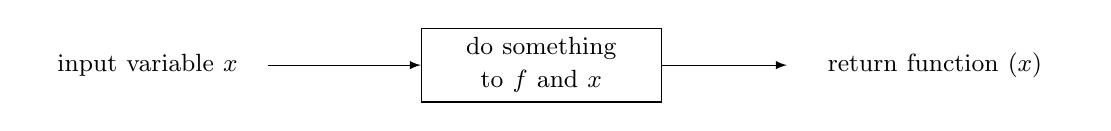
\begin{tikzpicture}[>=latex]
		\draw (-2,0) node (n1) [text width=80pt,align=center] {\small \centering input variable $x$ } 
					(3,0) node (n2) [draw,text width=80pt,align=center] {\small  \centering do something to $f$ and $x$}
					(8,0) node (n3) [text width=100pt,align=center] {\small \centering return function  $\fp(x)$};
		\draw [->] (n1) -- (n2);
		\draw [->] (n2) -- (n3);
		\end{tikzpicture}
		\end{center}
The output is the derivative function, $\fp(x)$. The $\fp(x)$ function will take a number $c$ as input and return the derivative of $f$ at $c$. This gives rise to the following definition.




\begin{definition}[Derivative function]\label{def:the_derivative}
Let $f$ be a differentiable function on an open interval $I$. The function 
$$\fp(x) = \lim_{h\to 0} \frac{f(x+h)-f(x)}{h}$$ 
is the derivative of $f$.\index{derivative ! as a function}\index[aut]{afgeleide ! van een functie}
\end{definition}



Note that the following notations all represent the derivative of a function $f$, if defined as $y = f(x)$:
$$\fp(x)\ =\ y'\ =\ \frac{dy}{dx}\ =\ \frac{df}{dx}\ =\ \frac{d}{dx}(f)\ =\ \frac{d}{dx}(y). $$


\begin{example}\label{ex_deriv1}
Find the derivative of the following functions:
\begin{multicols}{2}
\begin{enumerate}
\item  $f(x) = 3x^2+5x-7$
\item $f(x) = \sin(x)$
\end{enumerate}
\end{multicols}

\xhrulefill{gray}{2.5pt}Solution \xhrulefill{gray}{2.5pt}

\begin{enumerate}
\item We apply Definition \ref{def:the_derivative}.
	\begin{align*}
	\fp(x) &= \lim_{h\to 0} \dfrac{f(x+h)-f(x)}{h} \\[0.2cm]
					&=	\lim_{h\to 0} \dfrac{3(x+h)^2+5(x+h)-7-(3x^2+5x-7)}{h}\\[0.2cm]
					&=	\lim_{h\to 0} \dfrac{3h^2 +6xh+5h}{h}\\[0.2cm]
					&= \lim_{h\to 0} (3h+6x+5)\\
					&= 6x+5
	\end{align*}
	So $\fp(x) = 6x+5$. Recall earlier we found that $\fp(1) = 11$, which is affirmed by our new computation of $\fp(x)$. 
	\ifmathematica
	\ifcourse Moreover, we can verify the correctness of our computation using Mathematica. More precisely, we can compute derivatives in Mathematica using the built-in command \lstinline{D} as follows.
	\begin{mdframed}[default,backgroundcolor=gray!40,roundcorner=8pt]
\begin{mmaCell}[morefunctionlocal={x}]{Input}
  D[3*x^2+5*x-7,x]
\end{mmaCell}

\begin{mmaCell}{Output}
  5+6x
\end{mmaCell}
\end{mdframed}
The second argument of the command \lstinline{D} indicates the variable with respect to which the derivative is computed. 
\index{\lstinline{D}}\index[aut]{\lstinline{D}}
\fi
\fi

\ifpython
\ifcourse Moreover, we can verify the correctness of our computation using Python. More precisely, we can compute derivatives in Python using the built-in command \lstinline{diff} as follows.
\begin{pyin}
from sympy import symbols, diff
x = symbols('x')
diff(3*x**2 + 5*x - 7, x)
\end{pyin}
\begin{pyout}
6x+5
\end{pyout}
The second argument of the command \lstinline{D} indicates the variable with respect to which the derivative is computed.
\index{\lstinline{diff}}\index[aut]{\lstinline{diff}} \fi
\fi

\item We again apply Definition \ref{def:the_derivative},
$$
		\begin{array}{rcll}
		\fp(x) &=& \lim_{h\to 0} \dfrac{\sin(x+h)-\sin(x)}{h} & \\
		&&\left(\text{\scriptsize \parbox{110pt}{\centering Use trig identity $\sin(x+h) = \sin(x)\cos(h)+\cos(x)\sin(h)$}}\right)& \\[0.2cm]
						&=& \ds\lim_{h\to 0} \dfrac{\sin (x)\cos (h)+\cos (x)\sin (h)-\sin (x)}{h} &  \quad\text{(Sine of sum.)}\\[0.2cm]
						&=& \ds\lim_{h\to 0} \dfrac{\sin (x)(\cos (h)-1) + \cos (x)\sin (h)}{h} &  \quad\text{(Regroup.)}\\[0.2cm]
						&=& \lim_{h\to 0} \left(\dfrac{\sin (x)(\cos (h)-1)}{h} + \dfrac{\cos (x)\sin (h)}{h}\right)  &\quad\text{(Split into two fractions.)}\\[0.2cm]
						&&\left(\scriptsize\parbox{130pt}{use $\ds \lim_{h\to 0} \dfrac{\cos (h)-1}{h} = 0$ and $\ds \lim_{h\to 0} \dfrac{\sin (h)}{h} = 1$}\right)\\[0.2cm]
						&=&	\sin (x)\cdot 0 + \cos (x) \cdot 1 & \quad\text{(Special limits.)} \\
						&=& \cos (x)&
		\end{array}
$$
We have found that when $f(x) = \sin (x)$, $\fp(x) = \cos (x)$. This is not entirely surprising. The sine function is periodic -- it repeats itself on regular intervals. Therefore its rate of change also repeats itself on the same regular intervals.
\end{enumerate}
\end{example}


The next example illustrates that the derivative of a function may not always exist. 

\begin{example}\label{ex_not_diff}
Find the derivative of the absolute value function:
$$f(x) = |x| = \left\{\begin{array}{rcl} -x, & \mbox{if} & x<0, \\ x,  & \mbox{if} & x\geq 0. \end{array}\right.%\qquad \text{See Figure \ref{fig:absolutevalue}.}
$$
Its graph is shown in Figures~ \ref{fig_diff_3a}.

\xhrulefill{gray}{2.5pt}Solution \xhrulefill{gray}{2.5pt}

We need to evaluate $\ds \lim_{h\to0}\tfrac{f(x+h)-f(x)}{h}.$ As $f$ is piecewise--defined, we need to consider separately the limits when $x<0$,  $x>0$ and $x=0$. 

\begin{enumerate}
    \item When $x<0$ :
    \allowdisplaybreaks
	\begin{align*}
	\frac{d}{dx}\big(-x\big) 	&= \lim_{h\to 0}\frac{-(x+h) - (-x)}{h} \\[0.2cm]
														&=	\lim_{h\to 0}\frac{-h}{h}\\[0.2cm]
														&=	\lim_{h\to 0}(-1)=-1 \,.
	\end{align*}
 \item When $x>0$, a similar computation shows that $\ds \frac{d}{dx}\big(x\big) = 1$. 

 \item We need to also find the derivative at $x=0$. By the definition of the derivative at a point, we have $$\fp(0) = \lim_{h\to0}\frac{f(0+h)-f(0)}{h}\,.$$ Since $x=0$ is the point where our function's definition switches from one piece to the other, we need to consider left- and right-hand limits. Consider the following, where we compute the left- and right-hand limits side by side.

\noindent\begin{minipage}[b]{.5\linewidth}
\begin{align*}
&\lim_{h\underset{<}{\rightarrow}0}\frac{f(0+h)-f(0)}{h}\\
&=\quad\lim_{h\underset{<}{\rightarrow}0}\frac{-h-0}{h}  \\
&=\quad\lim_{h\underset{<}{\rightarrow}0}-1\;=\;-1
\end{align*}
\end{minipage}\rule{.5pt}{70pt}
\begin{minipage}[b]{.5\linewidth}
\begin{align*}
&\lim_{h\underset{>}{\rightarrow}0}\frac{f(0+h)-f(0)}{h} \\
&=\quad\lim_{h\underset{>}{\rightarrow}0}\frac{h-0}{h}  \\
&=\quad\lim_{h\underset{>}{\rightarrow}0}1\;=\;1
\end{align*}
\end{minipage}
		
Clearly, the left- and right-hand limits are not equal. Therefore the limit does not exist at 0, and $f$ is not differentiable at 0.
\end{enumerate}
Summarising, we have $$\fp(x) = \left\{\begin{array}{rcl} -1, & \mbox{if} & x<0, \\ 1, & \mbox{if} & x>0. \end{array}\right.$$ 
\ifcourse
\ifanalysis At $x=0$, $\fp(x)$ does not exist; there is a so-called jump discontinuity at 0 (Figure \ref{fig_diff_3b}). So $f(x) = |x|$ is differentiable everywhere except at 0. 
\fi
\ifcalculus At $x=0$, $\fp(x)$ does not exist; there is a  discontinuity at 0 (Figure \ref{fig_diff_3b}). So $f(x) = |x|$ is differentiable everywhere except at 0. 
\fi
\fi

\ifvc At $x=0$, $\fp(x)$ does not exist; there is a  discontinuity at 0 (Figure \ref{fig_diff_3b}). So $f(x) = |x|$ is differentiable everywhere except at 0. 
\fi

\begin{figure}[H]
\centering
%\raisebox{0.5cm}{
\subfigure[\label{fig_diff_3a}]{\includegraphics[width=0.4\textwidth]{fig_diff_3a}}
\qquad
\subfigure[\label{fig_diff_3b}]{\includegraphics[width=0.4\textwidth]{fig_diff_3b}}
\caption{The graph of $f(x)=\left|x\right|$ (a) and its derivative (b). }
\end{figure}


\end{example}

The point of non-differentiability came where the piecewise defined function switched from one piece to the other.



\ifcourse
Our next example shows that this does, however, not always cause trouble.
\ifanalysis\pagebreak\fi

\begin{example}\label{ex_diff_piecewise}
Find the derivative of $f(x)$, given by 
$$\ds f(x) = \left\{\begin{array}{cc} \sin(x), & x\leq \frac{\pi}{2} \\[0.2cm] 1, & x>\frac{\pi}{2}. \end{array}\right.$$
Its graph is shown in Figure \ref{fig_diff_4a}.

\xhrulefill{gray}{2.5pt}Solution \xhrulefill{gray}{2.5pt}

From Example \ref{ex_deriv1}, we know that when $x<\pi/2$, $\fp(x) = \cos (x)$. It is easy to verify that when $x>\pi/2$, $\fp(x) = 0$; consider:
			$$\lim_{h\to0}\frac{f(x+h) - f(x)}{h} = \lim_{h\to0}\frac{1-1}{h} = \lim_{h\to0}0 =0.$$

			
So far, we have $$\fp(x) = \left\{\begin{array}{cc} \cos(x) & x<\frac{\pi}{2}\\[0.2cm] 0 & x>\frac{\pi}{2}.\end{array}\right.$$ We still need to find $\fp(\pi/2)$. Notice at $x=\pi/2$ that both pieces of $\fp$ are 0, meaning we can state that $\fp(\pi/2)=0$. 

Being more rigorous, we can again evaluate the difference quotient limit at $x=\pi/2$, utilizing again left- and right--hand limits:\\


\noindent\begin{minipage}{.6\linewidth}
\begin{align*}
&\lim_{h\underset{<}{\rightarrow}0}\frac{f\left(\frac{\pi}{2}+h\right)-f\left(\frac{\pi}{2}\right)}{h} \\
&=\quad\lim_{h\underset{<}{\rightarrow}0}\frac{\sin\left(\frac{\pi}{2}+h\right)-\sin\left(\frac{\pi}{2}\right)}{h}\\
&=\quad\lim_{h\underset{<}{\rightarrow}0}{ \frac{\sin\left(\frac{\pi}{2}\right)\cos(h)+\sin(h)\cos\left(\frac{\pi}{2}\right)-\sin\left(\frac{\pi}{2}\right)}{h}}\\
&=\quad\lim_{h\underset{<}{\rightarrow}0}\frac{1\cdot\cos(h)+\sin(h)\cdot 0-1}{h} \\
&=\quad0\,.
\end{align*}
\end{minipage}
\begin{minipage}{1pt}
 \rule{.5pt}{100pt}
\end{minipage}
\begin{minipage}{.4\linewidth}
\begin{align*}
&\lim_{h\underset{>}{\rightarrow}0}\frac{f\left(\frac{\pi}{2}+h\right)-f\left(\frac{\pi}{2}\right)}{h}\\
&=\quad\lim_{h\underset{>}{\rightarrow}0}\frac{1-1}{h}\\
&=\quad\lim_{h\underset{>}{\rightarrow}0}\frac{0}{h}\\
&=\quad0\,.&\\
\phantom{0}\\
\phantom{0}
\end{align*}
\end{minipage}
\normalsize

Since both are 0 at $x=\pi/2$, the limit exists and $\fp(\pi/2)$ exists (and is 0). Therefore we can fully write $\fp$ as 
$$\fp(x) = \left\{\begin{array}{cc} \cos(x), & x\leq\frac{\pi}{2}\\[0.2cm] 0, & x>\frac{\pi}{2}.\end{array}\right.$$ 
See Figure \ref{fig_diff_4b} for a graph of this function.
\end{example}


%\ifanalysis\begin{figure}\fi
\begin{figure}[h]
\centering
\subfigure[\label{fig_diff_4a}]{\includegraphics[width=0.43\textwidth]{fig_diff_4a}}
\qquad
\subfigure[\label{fig_diff_4b}]{\includegraphics[width=0.43\textwidth]{fig_diff_4b}}
\caption{The graph of $f(x)$ as defined in Example \ref{ex_diff_piecewise} (a) and its derivative (b). }
\end{figure}

Loosely speaking, we defined a continuous function in Chapter~\ref{chap_limits} as one in which we could sketch its graph without lifting our pencil. Likewise, it can be understood that a function is differentiable if it is a continuous function that does not have any sharp corners. One such sharp corner is shown in Figure \ref{fig_diff_3a}. On the other hand, even though the function $f$ in Example \ref{ex_diff_piecewise} is piecewise--defined, the transition is smooth hence it is differentiable.


\ifanalysis

In general, we are guaranteed that a differentiable function is continuous through the following theorem. Be aware, however, that continuity does not imply differentiability. 

\begin{theorem}[Differentiable functions are continuous]
Let $f$ be differentiable in $c\in]a,b[$, then is $f$ continuous in $c$.
\end{theorem}

\begin{proof}
From Theorem~\ref{Caratheodory}, we know that for all  $x \in ]a,b[$ with $x \neq c$ it holds that:
$$
f(x) - f(c) = \frac{f(x) - f(c)}{x - c}(x - c).
$$
The limits for $x \longrightarrow c$ of both factors in the right-hand side of this exist, so 
$$
\lim_{x \rightarrow c} \left(f(x) - f(c)\right) = f'(c).0 = 0.
$$
This allows us to conclude that
$$
\lim_{x \rightarrow c} f(x) = f(c)\,,
$$
which on its turn implies that $f$ is continuous in $c$.
\end{proof}


\fi

\fi


\subsection{Differentiability on closed intervals}
When we defined the derivative at a point in Definition~\ref{def:derivative_at_a_point}, we specified that the interval $I$ over which a function $f$ was defined needed to be an open interval. Open intervals are required so that we can take a limit at any point $c$ in $I$, meaning we want to approach $c$ from both the left and right.

Recall we also required open intervals in Definition~\ref{def:continuous} when we defined what it meant for a function to be continuous. Later, we used one-sided limits to extend continuity to closed intervals. We now extend differentiability to closed intervals by again considering one-sided limits.

Our motivation for doing this is three-fold. First, we consider common sense. In Example \ref{ex_deriv1} we found that when $f(x) =  3x^2+5x-7$, $\fp(x) = 6x+5$, and this derivative is defined for all real numbers, hence $f$ is differentiable everywhere. It seems appropriate to also conclude that $f$ is differentiable on closed intervals, like $[0,1]$, as well. After all, $\fp(x)$ is defined at both $x=0$ and $x=1$. Secondly, consider $f(x) = \sqrt{x}$. The domain of $f$ is $\mathbb{R}^+$. It is natural to ask ourselves whether $f$ is differentiable on its domain -- specifically, is $f$ differentiable at $0$? Thirdly, having the derivative defined on closed intervals will prove  useful throughout the remainder of this chapter. 

Below we give a formal definition of differentiability on a closed interval.

\begin{definition}[Differentiability on a closed interval]\label{def:diff_closed}
Let $f$ be continuous on $[a,b]$ and differentiable on $]a,b[$, and let the one-sided limits 
$$\lim_{h\underset{>}{\rightarrow}0}\frac{f(a+h)-f(a)}{h}\quad\text{and}\quad\lim_{h\underset{<}{\rightarrow}0}\frac{f(b+h)-f(b)}{h}$$
 exist. Then we say $f$ is \textbf{differentiable} on $[a,b]$.
\end{definition}
\index{differentiable}\index[aut]{afleidbaar}\index{differentiability}\index[aut]{afleidbaarheid}
\index{left differentiable}\index[aut]{links afleidbaar}\index{right differentiable}\index[aut]{rechts afleidbaar}
\index{left derivative}\index[aut]{linkerafgeleide}\index{right derivative}\index[aut]{rechterafgeleide}


Given the notation of Definition~\ref{def:diff_closed} and in line with the terminology introduced for one-sided limits, we say that the function $f$ is \textbf{right differentiable} (\textit{rechts afleidbaar}) in $a$ and  \textbf{left differentiable} (\textit{links afleidbaar}) in $b$. Moreover, the one-sided limit\index{right differentiable}\index[aut]{rechts afleidbaar}\index{left differentiable}\index[aut]{links afleidbaar} 
$$\lim_{h\underset{>}{\rightarrow}0}\frac{f(a+h)-f(a)}{h}$$
is called the \textbf{right-derivative} (\textit{rechter afgeleide}) \index{right-derivative}\index[aut]{rechter afgeleide} of $f$ in $a$, while the one-sided limit
$$\lim_{h\underset{<}{\rightarrow}0}\frac{f(b+h)-f(b)}{h}$$
is referred to as the \textbf{left derivative} (\textit{linker afgeleide}) \index{left-derivative}\index[aut]{linker afgeleide} of $f$ in $b$.
 Using this terminology, we may say that a function $f$ is differentiable in $a$ if and only if it is left and right differentiable in $a$ and if its left and right derivatives in $a$ are equal.  

\begin{example}\label{ex_diff_closed1}
Consider the functions $f(x) = \sqrt{x}$ and $g(x) = \sqrt{x^3}$. The domain of these functions is $\mathbb{R}^+$ and it is easy to see that they are differentiable on $\mathbb{R}^+_0$. Determine the differentiability of each at $x=0$.

\xhrulefill{gray}{2.5pt}Solution \xhrulefill{gray}{2.5pt}

We start by considering $f$ and take the right-hand limit of the difference quotient:
\begin{align*}
\lim_{h\underset{>}{\rightarrow}0}\frac{f(a+h)-f(a)}{h} &= \lim_{h\underset{>}{\rightarrow}0}\frac{\sqrt{0+h}-\sqrt{0}}h \\
 &= \lim_{h\underset{>}{\rightarrow}0}\frac{\sqrt{h}}h\\
 &= \lim_{h\underset{>}{\rightarrow}0}\frac{1}{\sqrt{h}} = +\infty.
\end{align*}
The one-sided limit of the difference quotient does not exist at $x=0$ for $f$; therefore $f$ is differentiable on $\mathbb{R}^+_0$ and not differentiable on $\mathbb{R}^+$.

Now consider $g$:
\begin{align*}
\lim_{h\underset{>}{\rightarrow}0}\frac{g(a+h)-g(a)}{h} &= \lim_{h\underset{>}{\rightarrow}0}\frac{\sqrt{(0+h)^3}-\sqrt{0}}h \\
 &= \lim_{h\underset{>}{\rightarrow}0}\frac{h^{3/2}}h\\
 &= \lim_{h\underset{>}{\rightarrow}0}h^{1/2} = 0.
\end{align*}
As the one-sided limit exists at $x=0$, we conclude $g$ is differentiable on its domain of $\mathbb{R}^+$.

The two functions are graphed in Figure \ref{fig_diff_5}. Note how $f(x) = \sqrt{x}$ seems to go vertical as $x$ approaches 0, implying the slopes of its tangent lines are growing toward infinity.
Also note how the slopes of the tangent lines to $g(x)= \sqrt{x^3}$ approach 0 as $x$ approaches 0.


\begin{figure}[H]
	\begin{center}
			\includegraphics[width=0.5\textwidth]{fig_diff_5}
	\caption{A graph of $y=x^{1/2}$ and $y=x^{3/2}$.}
	\label{fig_diff_5}
	\end{center}
\end{figure}
\end{example}

\ifcourse

\subsection{Interpretations of the derivative}\label{sec:interp_deriv}
We offer two interconnected interpretations of the derivative, hopefully explaining why we care about it and why it is worthy of study.

\subsubsection{Instantaneous rate of change}
If $f$ is a function of $x$, then $\fp(x)$ measures the instantaneous rate of change of $f$ with respect to $x$. It is useful to recognize the units of the derivative function. If $y$ is a function of $x$, i.e., $y=f(x)$ for some function $f$, and $y$ is measured in metres and $x$ in seconds, then the units of $y' = \fp$ are metres per second. In general, if $y$ is measured in units $P$ and $x$ is measured in units $Q$, then $y'$ will be measured in units $P$ per $Q$.


Referring back to the falling amusement--park ride, knowing that at $t=2$ the velocity was $-64$ m/s, we could reasonably assume that 1 second later the riders' height would have dropped by about 64 metres. Knowing that the riders were accelerating as they fell would inform us that this is an under--approximation. If all we knew was that $f(2) = 86$ and $\fp(2) = -64$, we'd know that we'd have to stop the riders quickly otherwise they would hit the ground.




\begin{example}\label{ex_der_meaning1}
Let $P(t)$ represent the world population $t$ minutes after 12:00 a.m., January 1, 2012. It is fairly accurate to say that $P(0) = 7 028 734 178$ (\texttt{www.prb.org}). It is also fairly accurate to state that $P'(0) = 156$; that is, at midnight on January 1, 2012, the population of the world was growing by about 156 people per minute. Twenty days later (or, 28,800 minutes later) we could reasonably assume the population grew by about $28 800\cdot156 = 4 492 800$ people.
\end{example}

In this example we made use of the important approximation the rate of change was constant. Notationally, we would say that 
	$$f(c+h) \approx f(c) + \fp(c)\cdot h.$$ This approximation is best when $h$ is  small. Small is a relative term; when dealing with the world population, $h=$ 22 days = 28,800 minutes is small in comparison to years.
	
One of the most fundamental applications of the derivative is the study of motion. Let $s(t)$ be a position function, where $t$ is time and $s(t)$ is  distance. For instance, $s$ could measure the height of a projectile or the distance an object has travelled. Then $s'(t)$ has units metres per second, it measures the instantaneous rate of distance change -- it measures \textbf{velocity} (\textit{snelheid}).\index{velocity} \index[aut]{snelheid}

Now consider $v(t)$, a velocity function. That is, at time $t$, $v(t)$ gives the velocity of an object. The derivative of $v$, $v'(t)$, gives the instantaneous rate of velocity change -- \textbf{acceleration} (\textit{versnelling}).  If velocity is measured in metres per second, and time is measured in seconds, then the units of acceleration  are metres per second per second, or $($m/s$)$/s. We often shorten this to metres per second squared,  but this tends to obscure the meaning of the units.\index{acceleration}\index[aut]{versnelling}




\subsubsection{The slope of the tangent line}

Given a function $y=f(x)$, the difference quotient 
$$\ds \frac{f(c+h)-f(c)}{h}$$
 gives a change in $y$-values divided by a change in $x$-values; i.e., it is a measure of the slope of the line that goes through two points on the graph of $f$: $\big(c, f(c)\big)$ and $\big(c+h,f(c+h)\big)$. As $h$ shrinks to 0, these two points come close together; in the limit we find $\fp(c)$, the slope of a special line called the tangent line that intersects $f$ only once near $x=c$. Lines have a constant rate of change, their slope. Nonlinear functions do not have a constant rate of change, but we can measure their instantaneous rate of change at a given $x$ value $c$ by computing $\fp(c)$. We can get an idea of how $f$ is behaving by looking at the slopes of its tangent lines. 

% \begin{example}\label{ex_der_meaning3}
% Consider the function $f(x) = x^2$. At $x=3$ this function is growing faster than at $x=1$, as it is steeper at $x=3$. How much faster is it growing?

% \xhrulefill{gray}{2.5pt}Solution \xhrulefill{gray}{2.5pt}


% Here, we will answer this graphically, by considering the slopes of the respective tangent lines. One can sketch tangent lines to a curve at a particular point. In Figure \ref{fig_diff_6}, we have sketched the tangent lines to $f$ at $x=1$ and $x=3$, along with a grid to help us measure the slopes of these lines. At $x=1$, the slope is 2; at $x=3$, the slope is 6. Thus we can say not only is $f$ growing faster at $x=3$ than at $x=1$, it is growing three times as fast.

% \begin{figure}[H]
% 	\begin{center}
% 			\includegraphics[width=0.4\textwidth]{fig_diff_6}
% 	\caption{A graph of $f(x)=x^2$ and tangent lines at $x=1$ and $x=3$.}
% 	\label{fig_diff_6}
% 	\end{center}
% \end{figure}


% \end{example}

If we know $f(c)$ and $\fp(c)$ for some value $x=c$, then computing the tangent line at $(c,f(c))$ is easy: 
$$y=\ell(x) = \fp(c)(x-c)+f(c)\,.$$
It can then be used to approximate a value of $f$. More specifically, Let us use the tangent line at $x=c$ to approximate a value of $f$ near $x=c$; i.e., compute $\ell(c+h)$ to approximate $f(c+h)$, assuming again that $h$ is small. We get
$$y=\ell(c+h) = \fp(c)\big((c+h)-c\big)+f(c) = \fp(c)h + f(c).$$ 

\fi

\subsection{Higher-order derivatives}
The derivative of a function $f$ is itself a function, therefore we can take its derivative. The following definition gives a name to this concept and introduces its notation.

\begin{definition}[Higher-order derivatives]\label{def:Higher_Deriv}
Let $y=f(x)$ be a differentiable function on $I$. The following are defined, provided the corresponding limits exist. \index{derivative!higher order}\index{derivative!second}\index{derivative!third}\index{afgeleide! hogere orde}\index{afgeleide! tweede} \index{afgeleide! derde}
		\begin{enumerate}
		\item		The \textbf{second derivative} (\textit{tweede afgeleide}) of $f$ is: 
						$$ \fp'(x) = \frac{d}{dx}\Big(\fp(x)\Big) = \frac{d}{dx}\left(\frac{dy}{dx}\right) = \frac{d^2y}{dx^2}=y''.$$
				\item		The \textbf{third derivative} (\textit{derde afgeleide}) of $f$ is: 
						$$ \fp''(x) = \frac{d}{dx}\Big(\fp'(x)\Big) = \frac{d}{dx}\left(\frac{d^2y}{dx^2}\right) = \frac{d^3y}{dx^3}=y'''.$$
				\item		The \textbf{n$^{\text{th}}$ derivative} (\textit{$n$-de afgeleide}) of $f$ is:
						$$ f\,^{(n)}(x) = \frac{d}{dx}\left(f\,^{(n-1)}(x)\right) = \frac{d}{dx}\left(\frac{d^{n-1}y}{dx^{n-1}}\right) = \frac{d^ny}{dx^n}=y^{(n)}.$$
		\end{enumerate}
\end{definition}

In general, when finding the fourth derivative and so on, we resort to the $f\,^{(4)}(x)$ notation, not $\fp'''(x)$; because after a while, too many ticks is  confusing. Moreover, the second derivative notation could be written as 
$$\frac{d^2y}{dx^2}=\frac{d^2y}{(dx)^2}=\frac{d^2}{(dx)^2}\big(y\big).$$ 
That is, we take the derivative of $y$ twice (hence $d^2$), both times with respect to $x$ (hence $(dx)^2=dx^2$).
\ifmathematica
\ifcourse Also higher-order derivatives can be computed in Mathematica using the built-in command \lstinline{D}. For instance, the second derivative of $y=x^2$ can be computed as follows. 
	\begin{mdframed}[default,backgroundcolor=gray!40,roundcorner=8pt]
\begin{mmaCell}[morefunctionlocal={x}]{Input}
  D[x^2,\{x,2\}]
\end{mmaCell}

\begin{mmaCell}{Output}
  2
\end{mmaCell}
\end{mdframed}
The second argument of the function \lstinline{D} is now a list containing the focal variable and the order of the derivative. \index{\lstinline{D}}\index[aut]{\lstinline{D}}
\fi
\fi

\ifpython
\ifcourse Also higher-order derivatives can be computed in Python using the built-in command \lstinline{diff}. For instance, the second derivative of $y=x^2$ can be computed as follows. 
\begin{pyin}
from sympy import symbols, diff
x = symbols('x')
diff(x**2, x, 2)
\end{pyin}
\begin{pyout}
2
\end{pyout}
The second argument of the function \lstinline{diff} is now a list containing the focal variable and the order of the derivative.
\fi
\fi

But what do higher order derivatives mean? What is the practical interpretation?
Our first answer is
	\begin{quote}
	The second derivative of a function $f$ is the rate of change of the rate of change of $f$.
	\end{quote}

One way to grasp this concept is to let $f$ describe a position function. Then, $\fp$ describes the rate of position change: velocity. We now consider $\fp'$, which describes the rate of velocity change. Its derivative describes the  rate of change of the rate of position change, which we know as acceleration. It can, however, be difficult to consider the meaning of the third, and higher order, derivatives. The third derivative is the rate of change of the rate of change of the rate of change of $f$. That is essentially meaningless to the uninitiated. \ifcourse In the context of our position/velocity/acceleration example, the third derivative is the rate of change of acceleration, commonly referred to as jerk.

Make no mistake: higher-order derivatives have great importance even if their practical interpretations are hard to understand. The mathematical topic of series makes extensive use of higher-order derivatives \ifanalysis(Chapter~\ref{chap_series})\fi\ifcalculus(Section~\ref{sec:taylor_poly})\fi.\fi



\ifcourse
\subsection{Smoothness}
Some of the graphs  we encountered so far have sharp corners, or \textbf{cusps}, where the corresponding functions are not differentiable. This leads us to a definition.

\begin{definition}[Smoothness]\label{def:smooth}
A \textbf{smooth function} (\textit{gladde functie}) is a function that has continuous derivatives up to some desired order over some domain. A function can therefore be said to be smooth over a restricted interval $I$. Moreover, a function $f$ is \textbf{piecewise smooth} (\textit{stuksgewijs gladde functie}) on $I$ if $I$ can be partitioned into subintervals where $f$ is smooth on each subinterval.
\index{smooth!function}\index{cusp}\index[aut]{functie ! glad}\index{function ! smooth}\index{smoothness}
\end{definition}
	\checkoddpage
\marginpar{\ifoddpage\hspace*{-1.5cm}\else\hspace*{0.25cm}\fi\includegraphics[width=0.075\textwidth]{youtube}\\
\ifoddpage\hspace*{-1.75cm}\else\hspace*{0.1cm}\fi
\qrcode[height=1.75cm]{https://youtu.be/JR_6I9bvEIs}
%\includegraphics[width=0.1\textwidth]{smooth}
}
The number of continuous derivatives necessary for a function to be considered smooth depends on the problem at hand, and may vary from two to infinity. 

\ifanalysis

The function $f$ is said to be of (differentiability) \textbf{class $C^k$} (\textit{differentieerbaarheidsklasse}) if the derivatives $f'$, $f''$, \ldots, $f^{(k)}$ exist and are continuous. Note that the continuity is implied by differentiability for all the derivatives except for $f^{(k)}$. The function $f$ is said to be of class $C^{\infty}$, or \textbf{smooth} (\textit{glad}), if it has derivatives of all orders. Such a function is also called a \textbf{$C^{\infty}$-function}. To put it differently, the class $C^0$ consists of all continuous functions. The class $C^1$ consists of all differentiable functions whose derivative is continuous; such functions are called continuously differentiable. Thus, a $C^1$-function is exactly a function whose derivative exists and is of class $C^0$. 

For instance, the function
$$
\displaystyle f(x)={\begin{cases}x,&{\mbox{if }}x\geq 0,\\0,&{\text{if }}x<0\end{cases}}
$$
is continuous, but not differentiable at $x = 0$, so it is of class $C^0$ but not of class $C^1$.

The function
$$
\displaystyle g(x)={\begin{cases}x^{2}\sin {\left({\dfrac {1}{x}}\right)},&{\text{if }}x\neq 0,\\0,&{\text{if }}x=0\end{cases}}
$$
is differentiable, with derivative
$$
\displaystyle g'(x)={\begin{cases}-{\mathord {\cos\left({\dfrac {1}{x}}\right)}}+2x\sin\left({\dfrac {1}{x}}\right),&{\text{if }}x\neq 0,\\0,&{\text{if }}x=0.\end{cases}}
$$
Still, because $\cos \left(x^{-1}\right)$ oscillates as $x\to 0$, $g'(x)$ is not continuous at zero. Therefore, $g(x)$ is differentiable but not of class $C^1$.


\fi

\begin{example}
Determine whether or not the following functions are smooth.
\begin{multicols}{2}
\begin{enumerate}
\item $y=x^3$
\item $y= x\left|x\right|$
\end{enumerate}
\end{multicols}

\xhrulefill{gray}{2.5pt}Solution \xhrulefill{gray}{2.5pt}

\begin{enumerate}
\item We observe that the first derivative is given by $y'=3x^2$, the second derivative by $y''=6x$, the third derivative by $6$, while the fourth and higher-derivatives are all 0. Clearly, all these derivatives are continuous, so $y=x^3$ is a smooth function. 
\item For the sake of understanding, let us rewrite the equation as
$$
\displaystyle y={\begin{cases}x^2,&{\mbox{if }}x\geq 0,\\-x^2,&{\text{if }}x<0\,.\end{cases}}
$$
Its first derivative is given by
$$
\displaystyle y'={\begin{cases}2x,&{\mbox{if }}x\geq 0,\\-2x,&{\text{if }}x<0\,,\end{cases}}
$$
and is continuous everywhere. Yet, its second derivative,
$$
\displaystyle y''={\begin{cases}2,&{\mbox{if }}x\geq 0,\\-2,&{\text{if }}x<0\,\end{cases}}
$$
is not continuous everywhere, as there is a discontinuity at $x=0$. Consequently, this function is not smooth. \ifanalysis 
More specifically, it is a $C^1$-function because this functions derivatives exist and are continuous up to order 1. Hence, the first derivative of this function is a $C^0$-function. 
 \fi
\end{enumerate}
\end{example}




\fi



\section{Basic differentiation rules}\label{sec:basic_diff_rules}
The derivative is a powerful tool but is admittedly awkward given its reliance on limits. Fortunately, one thing mathematicians are good at is abstraction.

\subsection{Derivatives of algebraic and transcendental functions}
Let us consider a linear function, $y=mx+b$. What is $y'$? Without limits, recognize that linear function are characterized by being functions with a constant rate of change (the slope). The derivative, $y'$, gives the instantaneous rate of change; with a linear function, this is constant, $m$. Thus $y'=m$. 

Let us abstract once more. Let us find the derivative of the general quadratic function, $$f(x) = ax^2+bx+c\,.$$ Using the definition of the derivative, we have:
		\begin{align*}
		\fp(x) 	&=	\lim_{h\to 0}\frac{a(x+h)^2+b(x+h)+c-(ax^2+bx+c)}{h} \\[0.2cm]
						&=	\lim_{h\to 0} \frac{ah^2+2ahx+bh}{h} \\[0.2cm]
						&=	\lim_{h\to 0}(ah+2ax+b)\\[0.2cm]
						&= 2ax+b.
		\end{align*}
		
So if $y = 6x^2+11x-13$, we can immediately compute $y' = 12x+11$. 

In a similar way, using Definition~\ref{def:the_derivative} we can easily find the derivatives of the algebraic and transcendental functions we studied in Chapter~\ref{chap_algebraic} and \ref{chap_trans}, respectively. We find, for the constant function $f(x)=c$
$$
\ds \frac{d}{dx}\big( c\big) = 0\,,
$$
where $c\in\mathbb{R}$. This indicates the logical fact that constant functions have no rate of change. For the other algebraic functions we encountered we have 
\begin{itemize}
\item $\dfrac{d}{dx}\big(x^n\big) = nx^{n-1}\mbox{, where } n\in \mathbb{Z}$,
\item $\dfrac{d}{dx}\big(x^a\big) = ax^{a-1}\mbox{, where } a\in \mathbb{R}_0\mbox{ and } x>0$.
\end{itemize}
Hence, we immediately get 
$$
\dfrac{d}{dx}\big(\sqrt{x}\big) = \dfrac{1}{2\sqrt{x}},
$$
where $x>0$.

For what concerns the exponential and logarithmic functions, we get the following derivative functions:
\begin{multicols}{2}
\begin{itemize}
\item	$\dfrac{d}{dx}\left(e^x\right) = e^x$,	
\item	$\dfrac{d}{dx}\left(a^x\right) = a^x \ln(a), \text{ where } a>0 $,	
\item	$\dfrac{d}{dx}\left(\ln (x)\right) = \dfrac{1}{x}$,
\item	$\dfrac{d}{dx}\left(\log_a (x)\right) = \dfrac{1}{x \ln (a)}, \text{ where } a>0,  a \neq 1$,
\end{itemize}
\end{multicols}

\ifcourse
\ifanalysis 


while for the trigonometric and hyperbolic functions we get:

\begin{minipage}[t]{.49\linewidth}
\begin{itemize}
\item $\dfrac{d}{dx}\left(\sin(x)\right) = \cos(x),$ 
\item $\dfrac{d}{dx}\left(\cos(x)\right) = -\sin(x),$ 
\item $\dfrac{d}{dx}\left(\tan(x)\right) = \dfrac{1}{\cos^2(x)}=\sec^2(x),$ 
\item $\dfrac{d}{dx}\left(\cot(x)\right) = \dfrac{-1}{\sin^2(x)}=-\csc^2(x),$
%\item $\dfrac{d}{dx}\left(\sec(x)\right) = \dfrac{\sin(x)}{\cos^2(x)},$ 
%\item $\dfrac{d}{dx}\left(\csc(x)\right) = -\dfrac{\cos(x)}{\sin^2(x)},$
\end{itemize}
\end{minipage}
\begin{minipage}[t]{.49\linewidth}
\begin{itemize}
\item $\dfrac{d}{dx}\left(\sinh(x)\right) = \cosh(x),$ 
\item $\dfrac{d}{dx}\left(\cosh(x)\right) = \sinh(x),$ 
\item $\dfrac{d}{dx}\left(\tanh(x)\right) = \dfrac{1}{\cosh^2(x)},$ 
\item $\dfrac{d}{dx}\left(\coth(x)\right) = \dfrac{-1}{\sinh^2(x)}.$
\end{itemize}
\end{minipage}

\fi
\fi


\ifcalculus
while for the trigonometric functions we get:

\begin{minipage}[t]{.49\linewidth}
\begin{itemize}
\item $\dfrac{d}{dx}\left(\sin(x)\right) = \cos(x),$ 
\item $\dfrac{d}{dx}\left(\cos(x)\right) = -\sin(x),$ 
\end{itemize}
\end{minipage}
\begin{minipage}[t]{.49\linewidth}
\begin{itemize}
\item $\dfrac{d}{dx}\left(\tan(x)\right) = \dfrac{1}{\cos^2(x)}=\sec^2(x),$ 
\item $\dfrac{d}{dx}\left(\cot(x)\right) = \dfrac{-1}{\sin^2(x)}=-\csc^2(x).$
%\item $\dfrac{d}{dx}\left(\sec(x)\right) = \dfrac{\sin(x)}{\cos^2(x)},$ 
%\item $\dfrac{d}{dx}\left(\csc(x)\right) = -\dfrac{\cos(x)}{\sin^2(x)}.$
\end{itemize}
\end{minipage}
\fi

\ifvc
while for the trigonometric functions we get:

\begin{minipage}[t]{.49\linewidth}
	\begin{itemize}
		\item $\dfrac{d}{dx}\left(\sin(x)\right) = \cos(x),$ 
		\item $\dfrac{d}{dx}\left(\cos(x)\right) = -\sin(x),$ 
		\item $\dfrac{d}{dx}\left(\tan(x)\right) = \dfrac{1}{\cos^2(x)},$ 
	\end{itemize}
\end{minipage}
\begin{minipage}[t]{.49\linewidth}
	\begin{itemize}
		\item $\dfrac{d}{dx}\left(\cot(x)\right) = \dfrac{-1}{\sin^2(x)},$
		\item $\dfrac{d}{dx}\left(\sec(x)\right) = \dfrac{\sin(x)}{\cos^2(x)},$ 
		\item $\dfrac{d}{dx}\left(\csc(x)\right) = -\dfrac{\cos(x)}{\sin^2(x)}.$
	\end{itemize}
\end{minipage}
\fi

\ifcalculus
\begin{example}\label{ex_deriv_rule1}
Let $f(x)=x^3$. 
		\begin{enumerate}
		\item		Find $\fp(x)$.
		\item		Find the equation of the line tangent to the graph of $f$ at $x=-1$. 
		\item		Use the tangent line to approximate $(-1.1)^3$.
		\item		Sketch $f$, $\fp$ and the found tangent line at $x=-1$ on the same axis.
		\end{enumerate}

\ifcalculus\pagebreak\fi
\xhrulefill{gray}{2.5pt}Solution \xhrulefill{gray}{2.5pt}

\begin{enumerate}

		\item		Using the rule for differentiating a power function, we directly get $\fp(x) = 3x^2$. 

		\item		To find the equation of the line tangent to the graph of $f$ at $x=-1$, we need a point and the slope. The point is $(-1,f(-1)) = (-1, -1)$. The slope is $\fp(-1)= 3$. Thus the tangent line has equation $y = 3(x-(-1))+(-1) = 3x+2$. 
		
		\item		We can use the tangent line to approximate $(-1.1)^3$ as $-1.1$ is close to $-1$. We have $$(-1.1)^3 \approx 3(-1.1)+2 = -1.3.$$
			We can easily find the actual answer; $(-1.1)^3 = -1.331$. 
		
		\item		See Figure \ref{fig_diff_6}.
		\end{enumerate}
		
		\begin{figure}[H]
	\begin{center}
			\includegraphics[width=0.4\textwidth]{fig_diff_6}
	\caption{A graph of $f(x) = x^3$, along with its derivative $\fp(x) = 3x^2$ (gray) and its tangent line at $x=-1$ (dashed).}
	\label{fig_diff_6}
	\end{center}
\end{figure}


\end{example}
\fi

\subsection{Properties of the derivative}
Using the derivatives of the basic algebraic and transcendental functions, we can easily find the derivative of $y=x^3$, but we cannot compute the derivative of $y=2x^3$, $y=x^3+\sin (x)$ nor $y=x^3\sin (x)$. The following theorem helps with the first two of these examples.

\begin{theorem}[Properties of the derivative]\label{thm:deriv_prop}
Let $f$ and $g$ be differentiable on an open interval $I$ and let $c$ be a real number. Then the following properties hold:
	\begin{enumerate}
%	\item		\parbox{75pt}{\textbf{Sum/Difference Rule:}}\parbox[t]{176pt}{$\ds \frac{d}{dx}\Big(f(x) \pm g(x)\Big) = \frac{d}{dx}\Big(f(x)\Big) \pm \frac{d}{dx}\Big(g(x)\Big)$ $= \rule{0pt}{15pt}\fp(x)\pm g\primeskip'(x)$}
	\item	\textbf{Sum/Difference rule}:
	\begin{equation}
	\ds \frac{d}{dx}\Big(f(x) \pm g(x)\Big) = \frac{d}{dx}\Big(f(x)\Big) \pm \frac{d}{dx}\Big(g(x)\Big)=\fp(x)\pm g'(x).
	\label{afgeleidsom}
	\end{equation}
	\index{derivative ! sum/difference rule}\index[aut]{ afgeleide ! som/verschilregel}
	\item		\textbf{Constant multiple rule}:
	\begin{equation}
	\ds \frac{d}{dx}\Big(c\cdot f(x)\Big) = c\cdot\frac{d}{dx}\Big(f(x)\Big) = c\cdot\fp(x).
		\label{afgeleidcte}
	\end{equation}
	\end{enumerate}
\end{theorem}

\ifcourse
\ifanalysis

\begin{proof}
The sum rule, for instance, can be proved as follows. Let $f$ and $g$ be two functions that are differentiable in $a$, and  for which $\dom \,f \cap \dom\,g \neq \varnothing$. Then, for all  $h \neq 0$ and $a+h \in \dom\, f+g:$
$$ \begin{array}{lcl}
(f(a)+g(a))' &= &\ds\lim_{h\rightarrow 0}\dfrac{(f(a+h)+g(a+h))-(f(a)+g(a))}{h} \\
             &  & \\
             &= &\ds\lim_{h\rightarrow 0}\dfrac{f(a+h)-f(a)}{h}+\ds\lim_{h\rightarrow 0}
                 \dfrac{g(a+h)-g(a)}{h} \\
             &  &  \\
             &= &f'(a)+g'(a).
\end{array}$$
Consequently, for all $x \in \dom\, f+g$ Equation~\eqref{afgeleidsom} holds. 
\end{proof}

Intuitively, it is clear that the sum rule can be extended to $n$ functions $f_i(x)$; that is:
$$
\dfrac{d}{d x}\ds\left(\sum_{i=1}^nf_i(x)\right)=\ds\left(\sum_{i=1}^nf_i(x)\right)'=\ds\sum_{i=1}^nf'_i(x)\,.
$$


\fi
\fi

Theorem \ref{thm:deriv_prop} allows us to find the derivatives of a wide variety of functions. It can be used in conjunction with the power rule to find the derivatives of any polynomial. Recall in Example~\ref{ex_deriv1} that we found, using the limit definition, the derivative of $f(x) = 3x^2+5x-7$. We can now find its derivative without expressly using limits:
		\begin{align*}
		\frac{d}{dx}\Big(3x^2+5x+7\Big) &= 3\frac{d}{dx}\Big(x^2\Big) + 5\frac{d}{dx}\Big(x\Big) + \frac{d}{dx}\Big(7\Big) \\[0.2cm]
																		&= 3\cdot 2x+5\cdot 1+ 0\\
																		&= 6x+5.
		\end{align*}


\ifcalculus
\begin{example}\label{ex_high_order}
Find the first four derivatives of the following functions:
	
	
	\noindent\begin{minipage}[t]{.5\textwidth}
	\begin{enumerate}
	\item		$f(x) = 4x^2$
	\item		$g(x) = \sin (x)$
	\end{enumerate}
	\end{minipage}
	\noindent\begin{minipage}[t]{.5\textwidth}
	\begin{enumerate}\addtocounter{enumi}{2}
	\item		$h(x) = 5e^x$
	\end{enumerate}
	\end{minipage}

\xhrulefill{gray}{2.5pt}Solution \xhrulefill{gray}{2.5pt}

\begin{enumerate}
	\item		Using Theorem~\ref{thm:deriv_prop}, we have: $\fp(x) = 8x$. Continuing on, we have 
	$$\fp'(x) = \frac{d}{dx}\big(8x\big) = 8;\qquad \fp''(x) = 0;\qquad f\,^{(4)}(x) = 0.$$ Notice how all successive derivatives will also be 0.
	\item		Resorting repeatedly to the list of derivatives of elementary functions, we get the following:.
	$$g(x) = \cos x;\qquad g'(x) = -\sin x;\qquad g''(x) = -\cos x;\qquad g\,^{(4)}(x) = \sin x.$$ Note how we have come right back to $g(x)$ again. 
	\item		Again resorting  to the list of derivatives of elementary functions, we can see that $$h(x) = h'(x) = h''(x) = h\,^{(4)}(x) = 5e^x.$$
	\end{enumerate}
\end{example}

\fi 
When having to compute the derivative a product of functions, we may turn to the product rule. 


\begin{theorem}[Product rule]\label{thm:ProductRule}
Let $f$ and $g$ be differentiable functions on an open interval $I$.\index{product rule ! differentiation}\index{derivative ! product rule}\index[aut]{afgeleide ! productregel} Then $fg$ is a differentiable function on $I$, and
 $$\frac{d}{dx}\Big(f(x)g(x)\Big) = f(x)g'(x) + \fp(x)g(x).$$
\end{theorem}

\ifcourse
\ifanalysis

\begin{proof}
To prove Theorem \ref{thm:ProductRule}, we use the definition of the derivative. More specifically, by the limit definition, we have 
		$$\frac{d}{dx}\Big(f(x)g(x)\Big) =\lim_{h\to0} \frac{f(x+h)g(x+h)-f(x)g(x)}{h}.$$ 
	We now do something a bit unexpected; add 0 to the numerator (so that nothing is changed) in the form of $-f(x+h)g(x)+f(x+h)g(x)$, then do some regrouping as shown.
		\begin{align*}
		\frac{d}{dx}\Big(f(x)g(x)\Big) &=\lim_{h\to0} \frac{f(x+h)g(x+h)-f(x)g(x)}{h}\\[0.2cm]
																	&=	\lim_{h\to0} \frac{f(x+h)g(x+h)-f(x+h)g(x)+f(x+h)g(x)-f(x)g(x)}{h} \\[0.2cm]
																	&=	\lim_{h\to0} \frac{\Big(f(x+h)g(x+h)-f(x+h)g(x)\Big)+\Big(f(x+h)g(x)-f(x)g(x)\Big)}{h}\\[0.2cm]
																	&=	\lim_{h\to0} \frac{f(x+h)g(x+h)-f(x+h)g(x)}{h}+\lim_{h\to0}\frac{f(x+h)g(x)-f(x)g(x)}{h}\\[0.2cm]
																	&=\lim_{h\to0} f(x+h)\frac{g(x+h)-g(x)}{h}+\lim_{h\to0}\frac{f(x+h)-f(x)}{h}g(x)\\[0.2cm]
																	&=f(x)g'(x) + \fp(x)g(x).
		\end{align*}
\end{proof}


Just as with the sum rule, the product rule can be generalized to $n$ functions $f_i(x)$: 
\allowdisplaybreaks
\begin{align*}
\displaystyle {\frac {d}{dx}}\left[\prod _{i=1}^{n}f_{i}(x)\right]&=\sum _{i=1}^{n}\left({\frac {d}{dx}} (f_{i}(x))\prod _{j\neq i}f_{j}(x)\right)\\
&=\left(\prod _{i=1}^{n}f_{i}(x)\right)\left(\sum _{i=1}^{n}{\frac {f'_{i}(x)}{f_{i}(x)}}\right)\\
&= f'_1(x)f_2(x)f_3(x)\cdots f_n(x)+f_1(x)f'_2(x)f_3(x)\cdots f_n(x)+\cdots+f_1(x)f_2(x)f_3(x)\cdots f'_n(x)\,.
\end{align*}


\fi
\fi


\begin{example}\label{ex_prod1}
Find the derivatives of the following:
\begin{multicols}{3}
\begin{enumerate}
\item $y=5x^2\sin(x)$
\item $y = x^3\ln(x)\cos(x)$
\ifcourse
\ifanalysis \item $y=\cosh(x)e^x$\fi \fi
\end{enumerate}
\end{multicols}

\xhrulefill{gray}{2.5pt}Solution \xhrulefill{gray}{2.5pt}

\begin{enumerate}
\item To make our use of the product rule explicit, let us set $f(x) = 5x^2$ and $g(x) = \sin (x)$. We easily compute/recall that $\fp(x) = 10x$ and $g'(x) = \cos (x)$. Employing the product rule, we have 
$$\frac{d}{dx}\Big(5x^2\sin (x)\Big) = 5x^2\cos (x) + 10x\sin (x).$$
\item We have a product of three functions, so, we get
$$
y' = 3x^2\ln(x)\cos(x)  + x^3\frac{1}{x}\cos(x)+ x^3\ln(x)(-\sin(x))\,.
$$
\ifcourse
\ifanalysis \item Here we again have a product of two functions, so we immediately get
 $$y'=\sinh(x)e^x+\cosh(x)e^x\,.$$
 \fi \fi
\end{enumerate}
\end{example}

We have learned how to compute the derivatives of sums, differences, and products of functions. We now learn how to find the derivative of a quotient of functions.

\begin{theorem}[Quotient rule]\label{thm:QuotientRule}
Let $f$ and $g$ be differentiable functions defined on an open interval $I$, where $g(x) \neq 0$ on $I$.\index{derivative ! quotient rule}\index{quotient rule} Then $f/g$ is differentiable on $I$, and 
$$\frac{d}{dx}\left(\frac{f(x)}{g(x)}\right) = \frac{\fp(x)g(x) - f(x)g'(x)}{g(x)^2}.$$
\end{theorem}
\ifcourse
\ifanalysis 
\begin{proof}
The proof of the quotient rule follows easily using the properties introduced earlier. 
\end{proof}
\fi \fi

\begin{example}
Find the derivatives of the following:
\begin{multicols}{2}
\begin{enumerate}
\item $y = \dfrac{5x^2}{\sin(x)}$
\item $y = \tan(x)$
\end{enumerate}
\end{multicols}

\ifanalysis\pagebreak\fi
\xhrulefill{gray}{2.5pt}Solution \xhrulefill{gray}{2.5pt}

\begin{enumerate}
\item Directly applying the quotient rule gives:
	\begin{align*}
	y' &= \frac{10x\,\sin(x) - 5x^2\, \cos(x)}{\sin^2(x)}.
	\end{align*}
\item Though we could resort to the list of derivatives of elementary functions, we can proceed as well by recalling that $\tan (x) = \sin(x)/\cos(x)$, so we can apply the quotient rule.
\ifcalculus\allowdisplaybreaks\fi
		\begin{align*}
		\frac{d}{dx}\Big(\tan (x)\Big) &= \frac{d}{dx}\left(\frac{\sin (x)}{\cos (x)}\right) \\
																	&=	\frac{\cos (x) \cos (x) - \sin (x) (-\sin (x))}{\cos^2 (x)} \\[0.2cm]
																	&= \frac{\cos^2(x)+\sin^2(x)}{\cos^2(x)}\\[0.2cm]
																	&= \frac{1}{\cos^2(x)} \\[0.2cm]
																	&= \sec ^2 (x).
		\end{align*}
\end{enumerate}
\end{example}

The derivatives of the cotangent, cosecant and secant functions can all be computed  using the known derivatives of the cosine and sine function together with the quotient rule, so there is no need to learn those by heart.

Taking the derivative of many functions is relatively straightforward. It is clear  what rules apply and in what order they should be applied. Other functions present multiple paths; different rules may be applied depending on how the function is treated. One of the beautiful things about calculus is that there is not the right way; each path, when applied correctly, leads to the same result, the derivative.

\ifvc 
We demonstrate this concept in an example.

\begin{example}\label{ex_multiple_deriv}
Let 
$$\ds f(x) = \frac{x^2-3x+1}{x}.$$ Find $\fp(x)$ in each of the following ways:
		\begin{enumerate}
		\item		By applying the quotient rule,
		\item		by viewing $f$ as $f(x) = \big(x^2-3x+1\big)\, x^{-1}$ and applying the product and power rules, and
		\item		by simplifying first through division.
		\end{enumerate}

\xhrulefill{gray}{2.5pt}Solution \xhrulefill{gray}{2.5pt}

\begin{enumerate}
	\item		Applying the quotient rule gives: $$ \fp(x) = \frac{x\cdot\big(2x-3\big)-\big(x^2-3x+1\big)\, 1}{x^2} = \frac{x^2-1}{x^2} = 1-\frac{1}{x^2}.$$
	\item		By rewriting $f$, we can apply the product and power rules as follows:
			\begin{align*}
			\fp(x) &=		\big(x^2-3x+1\big)\cdot (-1)x^{-2} + \big(2x-3\big)\, x^{-1} \\[0.2cm]
							&=	-\frac{x^2-3x+1}{x^2}+\frac{2x-3}{x} \\[0.2cm]
							&= -\frac{x^2-3x+1}{x^2}+\frac{2x^2-3x}{x^2}\\[0.2cm]
							&= \frac{x^2-1}{x^2} = 1-\frac{1}{x^2},
			\end{align*}
			the same result as above.
	\item		As $x\neq 0$, we can divide through by $x$ first, giving $ f(x) = x-3+\frac{1}x$. Now apply the power rule. $$\fp(x) = 1-\frac{1}{x^2},$$  the same result as before.
	\end{enumerate}
\end{example}
\fi

\section{The chain rule}\label{sec:chainrule}

We have covered almost all of the derivative rules that deal with combinations of two (or more) functions.  The operations of addition, subtraction, multiplication (including by a constant) and division led to the sum,  difference, constant multiple, power rule, product and quotient rules. To complete the list of differentiation rules, we look at the last way two (or more) functions can be combined: the process of composition.

One example of a composition of functions is $f(x) = \cos(x^2)$. We currently do not know how to compute this derivative. If forced to guess, one would likely guess $\fp(x) = -\sin(2x)$, where we recognize $-\sin(x)$ as the derivative of $\cos(x)$ and $2x$ as the derivative of $x^2$. However, this is not the case; $\fp(x)\neq -\sin(2x)$.

Before we define this new rule, recall the notation for composition of functions. We write $(f \circ g)(x)$ or $f(g(x))$, read as $f$ of $g$ of $x$, to denote composing $f$ with $g$.  In shorthand, we simply write $f \circ g$ or $f(g)$ and read it as $f$ of $g$. When composing functions, we need to make sure that the new function is actually defined. For instance, consider $f(x) = \sqrt{x}$ and $g(x) = -x^2-1$. The domain of $f$ excludes all negative numbers, but the range of $g$ is only negative numbers. Therefore the composition $f\big(g(x)\big) = \sqrt{-x^2-1}$ is not defined for any $x$, and hence is not differentiable.

The following theorem of the \textbf{chain rule} (\textit{kettingregel}) takes care to ensure this problem does not arise. We'll focus more on the derivative result than on the domain/range conditions.

\begin{theorem}[The chain rule]\label{thm:chain_rule}
Let $g$ be a differentiable function on an interval $I$, let the range of $g$ be a subset of the interval $J$, and let $f$ be a differentiable function on $J$.
\index{derivative ! chain rule}\index{chain rule} Then $y=f(g(x))$ is a differentiable function on $I$, and 
$$y' = \fp(g(x))\, g'(x).$$%
\index[aut]{kettingregel}\index[aut]{afgeleide ! kettingregel}
\end{theorem} 

\ifcourse
\ifanalysis

\begin{proof}
This theorem can be proved by resorting to Theorem~\ref{Caratheodory} that provides us with an alternative viewpoint on differentiability.

First of all, putting $z_0=g(c)$, let us define an auxiliary function $q$ as follows:
$$
q:\dom\,f\to\mathbb{R}:z\mapsto\,q(z)=\left\{\begin{array}{rcl}
\dfrac{f(z)-f(z_0)}{z-z_0}&,&\text{ if }z\neq\,z_0\,,\\[0.2cm]
f'(z_0)&,&\text{ if }z=z_0\,.
\end{array}
\right.
$$ The function $q$ is continuous at $z_0$ since it holds that
$$
\ds\lim_{z\to\,z_0}q(z)=f'(z_0)=q(z_0)\,.
$$

Now, we may consider the composition $q\circ g$ for which $\dom(q\circ g)=\dom(f\circ g)$ because $\dom\,q=\dom\,f$. Given the definition of the function $q$, we have for this composition that 
$$
(q\circ g)(x)
=\left\{\begin{array}{rcl}
\dfrac{f(g(x))-f(g(c))}{g(x)-g(c)}&,&\text{ if }x\neq\,c\,,\\[0.2cm]
f'\left(g(c)\right)&,&\text{ if }x=c\,.
\end{array}\right.
$$

Finally, for all $x\neq c$ we may write
\begin{eqnarray*}
\dfrac{f(g(x))-f(g(c))}{x-c}&=&\dfrac{f(g(x))-f(g(c))}{g(x)-g(c)}\dfrac{g(x)-g(c)}{x-c}\\
&=&(q\circ g)(x)\dfrac{g(x)-g(c)}{x-c}\,.
\end{eqnarray*}

As we are looking for an expression for $(f\circ g)'(c)$, we consider the limit of both sides of the last expression for $x\to c$, which yields:
$$
(f\circ g)'(c)=\fp(g(c))\, g'(c)\,.
$$
\end{proof}
%Given the assumptions of the chain rule and the fact that differentiable functions and compositions of continuous functions are continuous, we have that there exist functions $q$, continuous at $g(c)$ and $r$, continuous at $c$, such that
%$$
%f\left(g(x)\right)-f\left(g(c)\right)=q\left(g(x)\right)\left(g(x)-g(c)\right)
%$$
%and
%$$
%g(x)-g(c)=r(x)(x-c)\,.
%$$
%Therefore,
%$$
%f\left(g(x)\right)-f\left(g(c)\right)=q\left(g(x)\right)r(x)(x-c)\,.$$
%
%Since the function $h(x)=q\left(g(x)\right)r(x)$ is continuous at $c$, we have at $c$ that
%$$
%f\left(g(c)\right)'=q\left(g(c)\right)r(c)=f'\left(g(c)\right)g'(c)\,.
%$$
% https://en.wikipedia.org/wiki/Chain_rule

\fi
\fi

\ifvc
\begin{example}\label{ex_chain2}
Find the derivatives of 
\begin{multicols}{2}
\begin{enumerate}
\item $y=(1-x)^2$
\item $g=(1-x)^3$
\end{enumerate}
\end{multicols}

\xhrulefill{gray}{2.5pt}Solution \xhrulefill{gray}{2.5pt}

\begin{enumerate}
\item We have that $y=(1-x)^2 = f(g(x))$,  where $f(x) = x^2$ and $g(x) = 1-x$. To find $y'$, we apply the chain rule. We need $\fp(x)=2x$ and $g'(x)=-1.$ Besides, part of the chain rule uses $\fp(g(x))$. This means substitute $g(x)$ for $x$ in the equation for $\fp(x)$. That is, $\fp(x) = 2(1-x)$.  Finishing out the chain rule we have $$y' = \fp(g(x))\ g'(x) = 2(1-x)\ (-1) = -2(1-x)= 2x-2.$$

\item Now, $y = (1-x)^3 = f(g(x))$, where $f(x) = x^3$ and $g(x) = (1-x)$. We have $\fp(x) = 3x^2$, so $\fp(g(x)) = 3(1-x)^2$. The chain rule then states $$y' = \fp(g(x))\ g'(x) = 3(1-x)^2(-1) = -3(1-x)^2.$$
\end{enumerate}

\end{example}

This example reveals that when $f(x)=x^n$, then $y' =n\ (g(x))^{n-1}\ g'(x)$. This  is called the generalized power rule and it follows from the chain rule.
\fi

\ifcourse
Acknowledging the chain rule, we can immediately state the so-called generalized power rule. 
\fi

\begin{theorem}[Generalized power rule]\label{thm:gen_power_rule}
Let $g(x)$ be a differentiable function and let $n\neq 0$ be an integer.\index{derivative ! power rule}\index{power rule}\index[aut]{productregel}\index[aut]{afgeleide ! productregel} Then $$\frac{d}{dx}\Big(g(x)^n\Big) = n \big(g(x)\big)^{n-1} g'(x).$$
\end{theorem}


It is instructive to understand what the  chain rule looks like using $\frac{dy}{dx}$ notation instead of $y'$ notation.  Suppose that $y=f(u)$ is a function of $u$, where $u=g(x)$ is a function of $x$, as stated in Theorem~\ref{thm:chain_rule}.  Then, through the composition $f \circ g$, we can think of $y$ as a function of $x$, as $y=f(g(x))$. Thus the derivative of $y$ with respect to $x$ makes sense; we can talk about $\frac{dy}{dx}.$  This leads to an interesting progression of notation:

\begin{align*}
y' &= \fp(g(x)) g'(x) \\
\frac{dy}{dx} &= \parbox{70pt}{$\ds y'(u)  u'(x)$} &\mbox{ (Since $y=f(u)$ and $u=g(x)$.)}\\
\frac{dy}{dx} &= \parbox{70pt}{$\ds \frac{dy}{du}  \frac{du}{dx}$ } &\mbox{ (Using fractional notation for the derivative.)}
\end{align*}

It might seem as though the $du$ terms cancel out, but it is important to realize that we are not cancelling these terms; the derivative notation of $\frac{dy}{du}$ is one symbol. It is equally important to realize that this notation was chosen precisely because of this behaviour. It makes applying the chain rule easy with multiple variables and/or with multiple functions. For instance, if we consider three functions  $y=f(u)$, $u=h(v)$ en $v=g(x)$, then we may consider the function composition $y=f(h(g(x)))$. The derivative of $y$ with respect to $x$ is then given by
 
$$\dfrac{dy}{dx}=\dfrac{dy}{du}\dfrac{du}{dv}\dfrac{dv}{dx}$$
or equivalently
$$\dfrac{dy}{dx}=\dfrac{df(u)}{du}\dfrac{dh(v)}{dv}\dfrac{dg(x)}{dx}\,.$$


We now consider some examples that employ the chain rule.

\ifcalculus
\begin{example}\label{ex_chain3}
Find the derivatives of the following functions:

		\begin{multicols}{3}
			\begin{enumerate}
			\item		$y = \sin{(2x)}$
			\item 	$y= \ln (4x^3-2x^2)$
   	\item	$y = e^{-x^2}$
	\end{enumerate}
	\end{multicols}


\xhrulefill{gray}{2.5pt}Solution \xhrulefill{gray}{2.5pt}
\begin{enumerate}
		\item		Consider $y = \sin(2x)$. Recognize that this is a composition of functions, where $f(u) = \sin(u)$ and $u=g(x) = 2x$. Thus $$y' = y'(u) u'(x) = \cos (u) 2 = 2\cos(2x).$$
		
		\item		Recognize that $y = \ln (4x^3-2x^2)$ is the composition of $f(u) = \ln(u)$ and $u=g(x) = 4x^3-2x^2$. This leads us to:
		$$y' = \frac{1}{4x^3-2x^2}  (12x^2-4x) = \frac{12x^2-4x}{4x^3-2x^2}= \frac{4x(3x-1)}{2x(2x^2-x)} = \frac{2(3x-1)}{2x^2-x}.$$
		
		\item		Recognize  that $y = e^{-x^2}$ is the composition of $f(u) = e^u$ and $u=g(x) = -x^2$. Remembering that $\fp(x) = e^x$, we have $$y' = e^{-x^2}(-2x) = (-2x)e^{-x^2}.$$
	\end{enumerate}
\end{example}

Of course, the chain rule can be applied in conjunction with any of the other rules we have already learned.
\fi

\begin{example}\label{ex_chain4}
Find the derivatives of the following: 
\begin{multicols}{2}
\begin{enumerate}
\item $y = x^5 \sin{(2x^3)}$
\item $y = \tan^5(6x^3-7x)$ 
\item $y = \dfrac{x\cos(x^{-2})-\sin^2(e^{4x})}{\ln(x^2+5x^4)}.$
\ifcourse
\ifanalysis\item $y=\tanh\left(\sinh(x)\right)$ \fi \fi
\end{enumerate}
\end{multicols}

\xhrulefill{gray}{2.5pt}Solution \xhrulefill{gray}{2.5pt}

\begin{enumerate}
\item		We must use the product and chain rules and proceed step--by--step.
		$$y' = x^5\big(6x^2\cos (2x^3)\big) + 5x^4\big(\sin (2x^3)\big)= 6x^7\cos(2x^3)+5x^4\sin(2x^3)\,.$$
\item Recognize that we have the $g(x)=\tan(6x^3-7x)$ function inside the $f(x)=x^5$ function. We begin using the generalized power rule; in this first step, we do not fully compute the derivative. Rather, we are approaching this step--by--step.
$$y' = 5\tan^4(6x^3-7x) g'(x).$$
We now find $g'(x)$. We again need the chain rule; $$g'(x) = \sec^2(6x^3-7x)(18x^2-7).$$ Combine this with what we found above to give
\begin{align*}
y' &= 5\tan^4(6x^3-7x)\sec^2(6x^3-7x)(18x^2-7)\\ 
&= (90x^2-35)\sec^2(6x^3-7x)\tan^4(6x^3-7x).
\end{align*}
\item Using the quotient, product and chain rules we get the following answer without simplification:
\begin{multline*}
y'=\frac{\ln(x^2+5x^4)\cdot\Big[\big(x(-\sin(x^{-2}))(-2x^{-3})+1 \cos(x^{-2})\big)-2\sin(e^{4x})\cos(e^{4x})(4e^{4x})\Big]}{\big(\ln(x^2+5x^4)\big)^2}\\[0.2cm]
-\frac{\Big(x\cos(x^{-2})-\sin^2(e^{4x})\Big)\cdot\frac{2x+20x^3}{x^2+5x^4}}{\big(\ln(x^2+5x^4)\big)^2}
\end{multline*}
\ifcourse
\ifanalysis\item Direct application of the chain rule with $g(x)=\sinh(x)$ inside the function $f(x)=\tanh(x)$ yields
$$ y=\dfrac{\cosh(x)}{\cosh^2\left(\sinh(x)\right)}\,.
$$
\fi \fi

\end{enumerate}
\end{example}

This example demonstrates that derivatives can be computed systematically, no matter how arbitrarily complicated the function is. A key to correctly working the considered problems is to break the problem down into smaller, more manageable pieces. For instance, when using the product and chain rules together, consider the first part of the product rule at first: $f(x)g'(x)$. Just rewrite $f(x)$, then find $g'(x)$. Then move on to the $\fp(x)g(x)$ part. Do not attempt to figure out both parts at once. Likewise, using the quotient rule, approach the numerator in two steps and handle the denominator after completing that. Only simplify afterwards.

The chain rule also has theoretic value. That is, it can be used to find the derivatives of certain functions.

\begin{example}\label{ex_chain8}
Use the chain rule to find the derivative of $y= 2^x$.

\xhrulefill{gray}{2.5pt}Solution \xhrulefill{gray}{2.5pt}

We only know how to find the derivative of one exponential function, $y = e^x$. %; this problem is asking us to find the derivative of functions such as $y = 2^x$. 
 We can accomplish our goal by rewriting $2$ in terms of $e$. Recalling that $e^x$ and $\ln x$ are inverse functions, so we can write
$$2=e^{\ln(2)} \quad \text{and so }\quad y=2^x = \big(e^{\ln(2)}\big)^x = e^{x(\ln(2))}.$$


The function is now the composition $y=f(g(x))$, with $f(u) = e^u$ and $g(x) = x(\ln(2))$.  Since $\fp(u) = e^u$ and $g'(x) = \ln(2)$, the chain rule  gives 

$$
y' = e^{x (\ln(2))}  \ln(2).
$$
Recall that the $e^{x(\ln(2))}$ term on the right hand side is just $2^x$, our original function. Thus, the derivative contains the original function itself. We have
$$
y' = y  \ln(2) = 2^x \ln(2).
$$
We can extend this process to use any base $a$, where $a>0$ and $a\neq 1$. All we need to do is replace each ``2'' in our work with ``$a$.'' In this way, the chain rule, coupled with the derivative rule of $e^x$, allows us to find the derivatives of all exponential functions.
\end{example}

The comment at the end of previous example is important. Let $f(x)=a^x$, for $a>0, a\neq 1$. Then $f$ is differentiable everywhere and 
$$\fp(x) = \ln (a) a^x\,.$$

Likewise, it can be shown that 
$$\frac{d}{dx}\big(\log_a (x)\big) = \frac{1}{\ln(a)}\frac{1}{x}\,.$$


\ifcourse

In the next section, we use the chain rule to justify another differentiation technique. There are many curves that we can draw in the plane that fail the vertical line test. See for instance Section~\ref{sec_conic}, where we studied amongst other things the equation $x^2+y^2=1$, which describes the unit circle. We may still be interested in finding slopes of tangent lines to the circle at various points. The next section shows how we can find $\frac{dy}{dx}$ without first solving for $y$.  While we can in this instance, in many other instances solving for $y$ is impossible. In these situations, implicit differentiation is indispensable. 
\fi



\ifcourse
\section{Implicit differentiation}\label{sec:imp_deriv}

\subsection{First derivative}
	\checkoddpage
\marginpar{\ifoddpage\hspace*{-1.5cm}\else\hspace*{0.25cm}\fi\includegraphics[width=0.075\textwidth]{youtube}\\
\ifoddpage\hspace*{-1.75cm}\else\hspace*{0.1cm}\fi
\qrcode[height=1.75cm]{https://youtu.be/qb40J4N1fa4}
%\includegraphics[width=0.1\textwidth]{implicit}
}

In the previous sections we learned to find the derivative when $y$ is given explicitly as a function of $x$. That is, if we know $y=f(x)$ for some function $f$, we can find $y'$. Sometimes the relationship between $y$ and $x$ is not explicit; rather, it is implicit. For instance, we might know that $x^2-y=4$.  Can we still find $y'$?  In this case, sure; we  solve for $y$ to get $y=x^2-4$  and then differentiate to get $y'=2x$. Sometimes, however, the implicit relationship between $x$ and $y$ is complicated.  Suppose we are given $\sin(y)+y^3=6-x^3$.  In this case there is absolutely no way to solve for $y$ in terms of elementary functions.  The surprising thing is, however, that we can still find $y'$ via implicit differentiation.\index{implicit differentiation}\index{derivative!implicit}\index{afleiden ! impliciet}

Implicit differentiation is a technique based on the chain rule that is used to find a derivative when the relationship between the variables is given implicitly rather than explicitly.

Let $f$ and $g$ be functions of $x$. Then we have according to the chain rule
 $$\frac{d}{dx}\Big(f(g(x))\Big) = \fp(g(x))\, g'(x).$$ 
Suppose now that $y=g(x)$. We can rewrite the above as 
\begin{equation}\frac{d}{dx}\Big(f(y)\Big) = \fp(y) y', \quad \text{or}\quad \frac{d}{dx}\Big(f(y)\Big)= \fp(y) \frac{dy}{dx} .\label{eq:implicit1}\end{equation} These equations look strange; the key concept to learn here is that we can find $y'$ even if we do not exactly know how $y$ and $x$ relate.

\begin{example}\label{ex_implicit1}
Given that 
$$\sin(y) + y^3=6-x^3\,,$$
find $y'$ and the equation of the tangent line at the point $(\sqrt[3]6,0)$.

\xhrulefill{gray}{2.5pt}Solution \xhrulefill{gray}{2.5pt}

We start by taking the derivative of both sides, which maintains the equality. We have :
$$ \frac{d}{dx}\Big(\sin(y) + y^3\Big)=\frac{d}{dx}\Big(6-x^3\Big).$$
The right-hand side is easy; it returns $-3x^2$. 

The left-hand side requires more consideration. We take the derivative term--by--term.  Using Equation~\eqref{eq:implicit1}, we can see that 
$$\frac{d}{dx}\Big(\sin(y)\Big) = \cos(y) \, y'.$$

We apply the same process to the $y^3$ term. 
$$\frac{d}{dx}\Big(y^3\Big) = \frac{d}{dx}\Big((y)^3\Big) = 3(y)^2\, y'.$$
Similarly, the derivative of $y^3$ is $3y^2y'$.  
Putting all this together with the right hand side, we have
$$\cos(y)y'+3y^2y' = -3x^2.$$
Now solve for $y'$.
		\begin{align*}
		\cos(y)y'+3y^2y' 	&= -3x^2\\
		\Leftrightarrow \quad \big(\cos (y)+3y^2\big)y' &=	-3x^2\\[0.2cm]
		\Leftrightarrow \hspace{2.9cm} y'&=	\frac{-3x^2}{\cos (y)+3y^2}
		\end{align*}


We can now find the slope of the tangent line at the point  $(\sqrt[3]6,0)$ by substituting $\sqrt[3]6$ for $x$ and $0$ for $y$. Thus at the point $(\sqrt[3]6,0)$, we have the slope as 
$$y' = \frac{-3(\sqrt[3]{6})^2}{\cos (0) + 3\cdot0^2} = \frac{-3\sqrt[3]{36}}{1} \approx -9.91.$$

Therefore the equation of the tangent line to the implicitly defined function $\sin y + y^3=6-x^3$ at the point $(\sqrt[3]{6},0)$ is $$y = -3\sqrt[3]{36}(x-\sqrt[3]{6})+0 \approx -9.91x+18.$$ The curve and this tangent line are shown in Figure~\ref{fig_diff_7}.

\begin{figure}[H]
	\begin{center}
			\includegraphics[width=0.4\textwidth]{fig_diff_7}
	\caption{The function $\sin y+y^3 = 6-x^3$ and its tangent line (dashed) at the point $(\sqrt[3]{6},0)$.}
	\label{fig_diff_7}
	\end{center}
\end{figure}

\end{example}

This example suggests a general method for implicit differentiation.  For the steps below assume $y$ is a function of $x$.
\begin{enumerate}
\item Take the derivative of each term in the equation.  Treat the $x$ terms like normal.  When taking the derivatives of $y$ terms, the usual rules apply except that, because of the chain rule, we need to multiply each term by $y'$.
\item Get all the $y'$ terms on one side of the equal sign and put the remaining terms on the other side.
\item Factor out $y'$;  solve for $y'$ by dividing.
\end{enumerate}


\begin{example}\label{ex_implicit5}
Given the implicitly defined function 
$$\sin(x^2y^2)+y^3=x+y,$$
find $y'$.

\ifanalysis\pagebreak\fi
\xhrulefill{gray}{2.5pt}Solution \xhrulefill{gray}{2.5pt}

Differentiating term by term, we find the most difficulty in the first term.  It requires both the chain and product rules.
		\begin{align*}
		\frac{d}{dx}\Big(\sin(x^2y^2)\Big) &= \cos(x^2y^2)\,\frac{d}{dx}\Big(x^2y^2\Big) \\
																				&= \cos(x^2y^2)\,\big(x^2(2yy')+2xy^2\big)\\
																				&= 2(x^2yy'+xy^2)\cos(x^2y^2).
		\end{align*}  

We leave the derivatives of the other terms to the reader. After taking the derivatives of both sides, we have
$$2(x^2yy'+xy^2)\cos(x^2y^2) + 3y^2y' = 1 + y'.$$

We now have to be careful to properly solve for $y'$, particularly because of the product on the left.  It is best to multiply out the product.  Doing this, we get
$$2x^2y\cos(x^2y^2)y' + 2xy^2\cos(x^2y^2) + 3y^2y' = 1 + y'.$$
From here we can safely move around terms to get the following:
$$2x^2y\cos(x^2y^2)y' + 3y^2y' - y' = 1 - 2xy^2\cos(x^2y^2).$$
Then we can solve for $y'$ to get
$$y' = \frac{1 - 2xy^2\cos(x^2y^2)}{2x^2y\cos(x^2y^2)+3y^2-1}.$$

A graph of this implicit function is given in Figure \ref{fig_diff_8}. It is easy to verify that the points $(0,1)$ and $(0,-1)$ all lie on the graph. We can find the slopes of the tangent lines at each of these points using our formula for $y'$: 
\begin{itemize}
\item at $(0,1)$, the slope is $1/2$;
\item at $(0,-1)$, the slope is also $1/2$.
\end{itemize}
The tangent lines have been added to the graph of the function in Figure \ref{fig_diff_8}.

\begin{figure}[H]
	\begin{center}
			\includegraphics[width=0.35\textwidth]{fig_diff_8}
	\caption{A graph of the implicitly defined function $\sin(x^2y^2)+y^3=x+y$ and tangent lines at  $(0,1)$ and $(0,-1)$.}
	\label{fig_diff_8}
	\end{center}
\end{figure}

\ifmathematica
We may also use Mathematica to check our answer for what concerns $y'$. We just have to be careful to explicitly mention the dependence of $y$ on $x$. 
	\begin{mdframed}[default,backgroundcolor=gray!40,roundcorner=8pt]
\begin{mmaCell}[morefunctionlocal={x}]{Input}
  D[Sin[x^2 y[x]^2] + y[x]^3 == x + y[x],x]
\end{mmaCell}

\begin{mmaCell}{Output}
  3 \mmaSup{y[x]}{2} \mmaSup{y}{\(\prime\)}[x]+Cos[\mmaSup{x}{2} \mmaSup{y[x]}{2}] (2 x \mmaSup{y[x]}{2}+2 \mmaSup{x}{2} y[x] \mmaSup{y}{\(\prime\)}[x])==1+\mmaSup{y}{\(\prime\)}[x]
\end{mmaCell}
\end{mdframed}
\index{\lstinline{D}}\index[aut]{\lstinline{D}}
\fi

\ifpython
We may also use Python to check our answer for what concerns $y'$. We just have to be careful to explicitly mention the dependence of $y$ on $x$.

\begin{pyin}
from sympy import symbols, function, diff
x = symbols('x')
y = Function('y')(x)
diff(sin(x**2 * y**2) + y**3 - x - y, x)
\end{pyin}
\begin{pyout}
\left(2x^2y(x)\frac{d}{dx}y(x) + 2xy^2(x)\right) \cos(x^2y^2(x)) + 3y^2(x)\frac{d}{dx}y(x) - \frac{d}{dx}y(x) - 1
\end{pyout}
\fi



\end{example}

Implicit functions are generally harder to deal with than explicit functions. With an explicit function, given an $x$ value, we have an explicit formula for computing the corresponding $y$ value. With an implicit function, one often has to find $x$ and $y$ values at the same time that satisfy the equation. It is much easier to demonstrate that a given point satisfies the equation than to actually find such a point.

\subsection{Higher-order derivatives}

We can use implicit differentiation to find higher-order derivatives as well. In theory, this is simple: first find $\frac{dy}{dx}$, then take its derivative with respect to $x$. In practice, it is not hard, but it often requires a bit of algebra. We demonstrate this in an example.


\begin{example}\label{ex_implicit9}
Given $x^2+y^2=1$, find $ y''$. 

\xhrulefill{gray}{2.5pt}Solution \xhrulefill{gray}{2.5pt}

Taking derivatives, we get $2x+2yy'=0$.  Solving for $y'$  gives: $$\ds y' = \frac{-x}{y}.$$ To find $y''$, we apply implicit differentiation to $y'$.
\ifcalculus\allowdisplaybreaks\fi
\begin{align*}
y'' &= \frac{d}{dx}\big(y'\big) \\
		&= \frac{d}{dx}\left(-\frac xy\right)\qquad\qquad\qquad\text{(Use the quotient rule.)} \\
		&= -\frac{y\cdot1 - x(y')}{y^2} \\
\intertext{replace $y'$ with $-x/y$:}
		&= -\frac{y-x(-x/y)}{y^2}\\
		&= -\frac{y+x^2/y}{y^2}\,.
\end{align*}
While this is not a particularly simple expression, it is usable. For instance, we can see that $y''>0$ when $y<0$ and $y''<0$ when $y>0$. In Section~\ref{sec:concavity}, we will see how this relates to the shape of the graph.
\end{example}

\subsection{Logarithmic differentiation}


Consider the function $y=x^x$; it is graphed in Figure \ref{fig_diff_9}. It is well defined for $x>0$ and we might be interested in finding equations of lines tangent and normal to its graph. How do we take its derivative?\index{logarithmic differentiation}\index{derivative!logarithmic differentiation}\index[aut]{logarithmisch afleiden}


\begin{figure}[h]
	\begin{center}
			\includegraphics[width=0.4\textwidth]{fig_diff_9}
	\caption{A plot of $y=x^x$.}
	\label{fig_diff_9}
	\end{center}
\end{figure}


The function is not a power function: it has a power of $x$, not a constant. It is not an exponential function: it has a base of $x$, not a constant.  A differentiation technique known as \textbf{logarithmic differentiation} (\textit{logaritmisch afleiden}) becomes useful here. The basic principle is this: take the natural log of both sides of an equation $y=f(x)$, then use implicit differentiation to find $y'$. We demonstrate this in the following example.


\begin{example}\label{ex_implicit10}
Given $y=x^x$, use logarithmic differentiation to find $y'$.

\pagebreak
\xhrulefill{gray}{2.5pt}Solution \xhrulefill{gray}{2.5pt}

We start by taking the natural log of both sides then applying implicit differentiation.
$$
\begin{array}{rrcll}
&y &=& x^x \\
\Leftrightarrow&\ln (y) &=& \ln (x^x)&\quad\text{(Apply logarithm rule.)}\\
\Leftrightarrow&\ln (y) &=& x\ln (x)& \quad\text{(Use implicit differentiation.)}\\ 
\Leftrightarrow&\dfrac{d}{dx}\Big(\ln (y)\Big) &=& \dfrac{d}{dx}\Big(x\ln (x)\Big) &\\[0.2cm]
\Leftrightarrow&\dfrac{y'}{y} &=& \ln (x) + x\,\dfrac1x&\\[0.2cm]
\Leftrightarrow&\dfrac{y'}{y} &=& \ln (x) + 1&\\
\Leftrightarrow&y' &=& y\big(\ln (x)+1\big)& \quad(y=x^x\,.)\\
\Leftrightarrow&y' &=& x^x\big(\ln (x)+1\big).
\end{array}
$$

\end{example}

\ifanalysis
The attentive reader might wonder at this point, whether logarithmic differentiation still works if $f(x)<=$ because we may not take the logarithm then. It turns out that it does because yo can consider $\ln|f(x)|$, which works for negative and positive values of any function $f(x)$. Where f(x)<0, we have that 
$
\ln|f(x)|=\ln(-f(x))
$
and the derivative
$$
\dfrac{d}{dx}\left(\ln(-f(x))\right)=\dfrac{1}{-f(x)}(-f'(x))=\dfrac{f'(x)}{f(x)}\,,
$$
which is the same as the derivative of $\ln(f(x))$, but just also works for negative values of $f(x)$. 
\fi

\fi



\section{Derivatives of inverse functions}\label{sec:deriv_inverse_function}

Recall that a function $y=f(x)$ is said to be injective if it passes the horizontal line test; that is, for two different $x$ values $x_1$ and $x_2$, we do not have $f(x_1)=f(x_2)$. In some cases the domain of $f$ must be restricted so that it is injective. For instance, consider $f(x)=x^2$. Clearly, $f(-1)= f(1)$, so $f$ is not one to one on its regular domain, but by restricting $f$ to $\mathbb{R}^+_0$, $f$ is one to one.\index{derivative ! inverse function}\index[aut]{afgeleide ! inverse functie}

Now recall that injective functions have inverses. That is, if $f$ is one to one, it has an inverse function, denoted by $f^{-1}$, such that if $f(a)=b$, then $f^{-1}(b) = a$. The domain of $f^{-1}$ is the range of $f$, and vice-versa. For ease of notation, we set $g=f^{-1}$ and treat $g$ as a function of $x$.

When the point $(a,b)$ lies on the graph of $f$, the point $(b,a)$ lies on the graph of $g$. This made us to discover in Section~\ref{sec_inverse} that the graph of $g$ is the reflection of $f$ across the line $y=x$. Because of this relationship, whatever we know about $f$ can quickly be transferred into knowledge about $g$.

For example, consider Figure~\ref{fig_diff_10} where the tangent line to $f$ at the point $(a,b)$ is drawn. That line has slope $\fp(a)$. Through reflection across $y=x$, we can see that the tangent line to $g$ at the point $(b,a)$ should have slope $\frac{1}{\fp(a)}$. This then tells us that $ g'(b) = \frac{1}{\fp(a)}.$


\begin{figure}
	\begin{center}
			\includegraphics[width=0.5\textwidth]{fig_diff_10}
	\caption{Corresponding tangent lines drawn to $f$ and $f^{-1}$.}
	\label{fig_diff_10}
	\end{center}
\end{figure}

We have discovered a relationship between $\fp$ and $g'$ in a mostly graphical way. We can realize this relationship analytically as well. Let $y = g(x)$, where again $g = f^{-1}$. We want to find $\ds y'$. Since $y = g(x)$, we know that $f(y) = x$. Using the chain rule and implicit differentiation, take the derivative of both sides of this last equality:
		$$
		\begin{array}{rrcl} 
			&\dfrac{d}{dx}\Big(f(y)\Big) &=& \dfrac{d}{dx}\Big(x\Big) \\[0.3cm]
			\Leftrightarrow& \fp(y)\, y' &=& 1\\
			\Leftrightarrow& y' &=& \dfrac{1}{\fp(y)}\\
			\Leftrightarrow& y' &=& \dfrac{1}{\fp(g(x))}.
		\end{array}
		$$
\ifcalculus\pagebreak\fi
This leads us to the following theorem.

\begin{theorem}[Derivatives of inverse functions]\label{thm:deriv_inverse_functions}
Let $f$ be differentiable and injective on an open interval $I$, where $\fp(x) \neq 0$ for all $x$ in $I$, let $J$ be the range of $f$ on $I$, let $g$ be the inverse function of $f$, and let $f(a) = b$ for some $a$ in $I$. Then $g$ is a differentiable function on $J$, and in particular,
	
\begin{center}
\hskip-7pt	\begin{tabular}{ccc}
	1. $\ds \left(f^{-1}\right)'(b)=g'(b) = \frac{1}{\fp(a)}$ &\hskip 4pt and \hskip 4pt&  2. $\ds \left(f^{-1}\right)'(x)=g'(x) = \frac{1}{\fp(g(x))}$
	\end{tabular}
\end{center}
\end{theorem}


The results of Theorem~\ref{thm:deriv_inverse_functions} are not trivial; the notation may seem confusing at first. Careful consideration, along with examples, should earn understanding.

In the next example we apply Theorem~\ref{thm:deriv_inverse_functions} to the arcsine function.

\begin{example}\label{ex_deriv_arcsin}
Let $y = \arcsin(x)$. Find $y'$.


\xhrulefill{gray}{2.5pt}Solution \xhrulefill{gray}{2.5pt}

Adopting our previously defined notation, let $g(x) = \arcsin(x)$ and $f(x) = \sin(x)$. Consequently, $\fp(x) = \cos(x)$. Applying the theorem, we have 
\begin{align*}
			g'(x) &= \frac{1}{\fp(g(x))} \\
						&= \frac{1}{\cos(\arcsin (x))} \,.
\end{align*}
			
This last expression is not immediately illuminating. Drawing a figure while assuming that $x>$ will help, as shown in Figure~\ref{fig_diff_11}. 

\begin{figure}[H]
	\begin{center}
			\includegraphics[width=0.5\textwidth]{fig_diff_11}
	\caption{A right triangle defined by $y=\arcsin(x/1)$ with the length of the third leg found using the Pythagorean theorem.}
	\label{fig_diff_11}
	\end{center}
\end{figure}

Recall that the sine function can be viewed as taking in an angle and returning a ratio of sides of a right triangle, specifically, the ratio opposite over hypotenuse. This means that the arcsine function takes as input a ratio of sides and returns an angle. The equation $y=\arcsin (x)$ can be rewritten as $y=\arcsin (x/1)$; that is, consider a right triangle where the hypotenuse has length 1 and the side opposite of the angle with measure $y$ has length $x$. This means the final side has length $\sqrt{1-x^2}$, using the Pythagorean theorem.


Therefore 
$$\cos (\arcsin(x)) = \cos(y) = \dfrac{\sqrt{1-x^2}}{1} = \sqrt{1-x^2},$$
resulting in $$\frac{d}{dx}\big(\arcsin(x)\big) = g'(x) = \frac{1}{\sqrt{1-x^2}}.$$

Remember that the input $x$ of the arcsine function is a ratio of a side of a right triangle to its hypotenuse; the absolute value of this ratio will never be greater than 1. Therefore the inside of the square root will never be negative.



\end{example}

Using similar techniques as in Example~\ref{ex_deriv_arcsin}, we can find the derivatives of all the inverse trigonometric \ifcourse \ifanalysis  and hyperbolic functions.  \fi \fi

The inverse trigonometric functions are differentiable on all open sets contained in their domains (as listed in Table~\ref{tab_res_tri}) and their derivatives are as follows:

	\begin{minipage}{.5\textwidth}
	\begin{itemize}
	\item		$\ds \frac{d}{dx}\big(\arcsin (x) \big) = \frac{1}{\sqrt{1-x^2}},$ 
	\item		$\ds \frac{d}{dx}\big(\arccos (x) \big) = -\frac{1}{\sqrt{1-x^2}},$ 
	\end{itemize}
	\end{minipage}
	\begin{minipage}{.5\textwidth}
	\begin{itemize}
	\item		$\ds \frac{d}{dx}\big(\arctan (x) \big) = \frac{1}{1+x^2}.$
	\item		$\ds \frac{d}{dx}\big(\arccot (x) \big) = -\frac{1}{1+x^2},$
	%\item		$\ds \frac{d}{dx}\big(\arcsec (x) \big) = \frac{1}{|x|\sqrt{x^2-1}},$
	%\item		$\ds \frac{d}{dx}\big(\arccsc (x) \big) = -\frac{1}{|x|\sqrt{x^2-1}}.$
	\end{itemize}
	\normalsize
	\end{minipage}

\ifcourse	
\ifanalysis

The derivatives of the inverse hyperbolic functions are as follows:

\begin{minipage}{.5\textwidth}
\begin{itemize}
\item $\ds \frac{d}{dx}\big(\arsinh(x)\big)=\frac {1}{\sqrt {x^{2}+1}}$,
\item $\ds \frac{d}{dx}\big(\arcosh(x)\big)=\frac {1}{\sqrt {x^{2}-1}}$, for all $x>1$,
\end{itemize}
\end{minipage}
\begin{minipage}{.5\textwidth}
\begin{itemize}
\item $\ds \frac{d}{dx}\big(\artanh(x)\big)=\frac {1}{1-x^{2}}$,  for all $|x|<1$,
\item $\ds \frac{d}{dx}\big(\arcoth(x)\big)=\frac {1}{1-x^{2}}$,  for all $|x|>1$.
%\item $\ds \frac{d}{dx}\big(\arsech(x)\big)=\frac {-1}{x{\sqrt {1-x^{2}}}}$, for all $ x\in \left.\right]0,1\left[\right.$,
%\item $\ds \frac{d}{dx}\big(\arcsch(x)\big)=\frac {-1}{|x|{\sqrt {1+x^{2}}}}$ , for all $x\neq0$.
\end{itemize}
\end{minipage}

\fi
\fi

In Section \ref{sec:basic_diff_rules}, we stated without proof or explanation that $\frac{d}{dx}\left(\ln (x)\right) = \frac{1}{x}$. We can justify that now using Theorem \ref{thm:deriv_inverse_functions}, as shown in the following example.

\begin{example}\label{ex_deriv_lnx}
Use Theorem \ref{thm:deriv_inverse_functions} to compute 
$$\dfrac{d}{dx}\left(\ln (x)\right).$$

\xhrulefill{gray}{2.5pt}Solution \xhrulefill{gray}{2.5pt}

View $y= \ln (x)$ as the inverse of $y = e^x$. Therefore, using our standard notation, let $f(x) = e^x$ and $g(x) = \ln (x)$. We wish to find $g'(x)$. Theorem \ref{thm:deriv_inverse_functions} gives:
		\begin{align*}
		g'(x) &= \frac{1}{\fp(g(x))} \\[0.2cm]
					&=	\frac{1}{e^{\ln (x)}}\rule{0pt}{15pt} \\[0.2cm]
					&= \frac{1}{x}.\rule{0pt}{17pt}
		\end{align*}
\end{example}


\ifcourse
\section{L'H\^opital's rule}\label{sec:lhopitals_rule}

Our treatment of limits in Chapter~\ref{chap_limits} exposed us to the notion of 0/0, an indeterminate form. If $\ds \lim_{x\to c}f(x)=0$ and $\ds \lim_{x\to c} g(x) =~0$, we do not conclude that $\ds \lim_{x\to c} f(x)/g(x)$ is $0/0$; rather, we use $0/0$ as notation to describe the fact that both the numerator and denominator approach 0. The expression 0/0 has no numeric value; other work must be done to evaluate the limit.

Other indeterminate forms exist; they are: %Limits may seeming evaluate to
 $\infty/\infty$, $0\cdot\infty$, $\infty-\infty$, $0^0$, $1^\infty$ and $\infty^0$. %, expressions which have no inherent value. 
 Just as 0/0 does not mean divide 0 by 0, the expression $\infty/\infty$ does not mean divide infinity by infinity. Instead, it means a quantity is growing without bound and is being divided by another quantity that is growing without bound. We cannot determine from such a statement what value, if any, results in the limit. 


\subsection{Indeterminate forms 0/0 and $\infty/\infty$}
Here, we introduce l'H\^opital's rule, a method of resolving limits that produce the indeterminate forms 0/0 and $\infty/\infty$. We will also show how algebraic manipulation can be used to convert other indeterminate expressions into one of these two forms so that our new rule can be applied.

\begin{theorem}[L'H\^opital's rule for 0/0]\label{thm:LHR}
Let $\ds \lim_{x\to c}f(x) = 0$ and $\ds \lim_{x\to c}g(x)=0$, where $f$ and $g$ are differentiable functions on an open interval $I$ containing $c$, and $g'(x)\neq 0$ on $I$ except possibly at $c$. Then \index{limit!L'H\^opital's Rule}\index{L'H\^opital's Rule}\index[aut]{L'H\^opital} \index[aut]{limiet ! L'H\^opital}
$$ \lim_{x\to c} \frac{f(x)}{g(x)} = \lim_{x\to c} \frac{\fp(x)}{g'(x)}.$$
\end{theorem}

\ifanalysis

\begin{proof}
In order to prove this theorem, suppose that $f$ and $g$ are continuously differentiable at a real number $c$, that $f(c)=g(c)=0$, and that $g'(c)\neq 0$. Then
$$
\displaystyle \lim _{x\to c}{\dfrac {f(x)}{g(x)}}=\lim _{x\to c}{\dfrac {f(x)-0}{g(x)-0}}\,,
$$
and since $f(c)=g(c)=0$, the latter expression equals
$$
\lim _{x\to c}{\dfrac {f(x)-f(c)}{g(x)-g(c)}}\\[6pt].
$$
Dividing both numerator and denominator of this expression by $x-c$ yields
$$
\lim _{x\to c}{\dfrac {\left({\dfrac {f(x)-f(c)}{x-c}}\right)}{\left({\dfrac {g(x)-g(c)}{x-c}}\right)}}={\dfrac {\lim \limits _{x\to c}\left({\dfrac {f(x)-f(c)}{x-c}}\right)}{\lim \limits _{x\to c}\left({\dfrac {g(x)-g(c)}{x-c}}\right)}}\,,
$$
or by relying on the difference quotient definition of the derivative and acknowledging continuity of the derivatives at $c$, we get 
$$
{\frac {f'(c)}{g'(c)}}=\lim _{x\to c}{\dfrac {f'(x)}{g'(x)}}.
$$
 The limit in the conclusion is not indeterminate because $g'(c)\neq 0$. 
\end{proof}

\fi





We demonstrate the use of l'H\^opital's rule (LHR) in the following examples.

\begin{example}\label{ex_lhr1}
Evaluate the following limits.

\noindent%
\begin{minipage}[t]{.5\textwidth}
\begin{enumerate}
\item		$\ds \lim_{x\to0}\frac{\sin (x)}x$
\item		$\ds \lim_{x\to 1}\frac{\sqrt{x+3}-2}{1-x}$
\end{enumerate}
\end{minipage}
\begin{minipage}[t]{.5\textwidth}
\begin{enumerate}\addtocounter{enumi}{2}
\item		$\ds \lim_{x\to0}\frac{x^2}{1-\cos (x)}$
\end{enumerate}
\end{minipage}

\ifcalculus\pagebreak\fi
\xhrulefill{gray}{2.5pt}Solution \xhrulefill{gray}{2.5pt}

\begin{enumerate}
\item		We proved this limit is 1 in Example \ref{ex_limit_sinx_prove} using the squeeze theorem. Here we use l'H\^opital's rule to show its power.
$$\lim_{x\to0}\frac{\sin (x)}x \stackrel{\ \text{ by LHR \rule[-5pt]{0pt}{3pt}} \ }{=} \lim_{x\to0} \frac{\cos (x)}{1}=1.$$

\item	\hfill $\ds \lim_{x\to 1}\frac{\sqrt{x+3}-2}{1-x} 	 \stackrel{\ \text{ by LHR \rule[-5pt]{0pt}{3pt}} \ }{=} \lim_{x \to 1} \frac{\frac12(x+3)^{-1/2}}{-1} =-\frac 14.$\hfill\null 

\item		\hfill $\ds \lim_{x\to 0}\frac{x^2}{1-\cos (x)}  \stackrel{\ \text{ by LHR \rule[-5pt]{0pt}{3pt}} \ }{=}  \lim_{x\to 0} \frac{2x}{\sin (x)}.$ \hfill\null

This latter limit also evaluates to the 0/0 indeterminate form. To evaluate it, we apply l'H\^opital's rule again.

\hfill $\ds  \lim_{x\to 0} \frac{2x}{\sin (x)}  \stackrel{\ \text{ by LHR \rule[-5pt]{0pt}{3pt}} \ }{=} \lim_{x\to0}\frac{2}{\cos (x)} = 2 .$ \hfill\null

Thus $\ds \lim_{x\to0}\frac{x^2}{1-\cos (x)}=2.$

\end{enumerate}
\end{example}

Note that at each step where l'H\^opital's rule was applied, it was needed: the initial limit returned the indeterminate form of $0/0$. If the initial limit returns, for example, 1/2, then l'H\^opital's rule does not apply.



The following theorem extends our initial version of l'H\^opital's rule in two ways. It allows the technique to be applied to the indeterminate form $\infty/\infty$ and to limits where $x$ approaches $\pm\infty$.

\begin{theorem}[L'H\^opital's rule for $\infty/\infty$]\label{thm:LHR2}

\begin{enumerate}
\item		Let $\ds\lim_{x\to a}f(x) = \pm\infty$ and $\ds\lim_{x\to a}g(x)=\pm \infty$, where $f$ and $g$ are differentiable on an open interval $I$ containing $a$. Then \index{limit!L'H\^opital's Rule}\index{L'H\^opital's Rule} \index[aut]{L'H\^opital} \index[aut]{limiet ! L'H\^opital}
$$\lim_{x\to a} \frac{f(x)}{g(x)} = \lim_{x\to a}\frac{\fp(x)}{g'(x)}.$$

\item		Let $f$ and $g$ be differentiable functions on the open interval $]a,+\infty[$ for some value $a$, where $g'(x)\neq 0$ on $]a,+\infty[$ and $\ds\lim_{x\to+\infty} f(x)/g(x)$ returns either ``0/0'' or ``$\infty/\infty$''. Then
$$\lim_{x\to+\infty} \frac{f(x)}{g(x)} = \lim_{x\to +\infty}\frac{\fp(x)}{g'(x)}.$$
A similar statement can be made for limits where $x$ approaches $-\infty$.
\end{enumerate}
\end{theorem}

\begin{example}\label{ex_LHR2}
Evaluate the following limits.

\begin{multicols}{2}
\begin{enumerate}
\item $\ds \lim_{x\to+\infty} \frac{3x^2-100x+2}{4x^2+5x-1000}$
\item $\ds\lim_{x\to+\infty}\frac{e^x}{x^3}$
\end{enumerate}
\end{multicols}

\xhrulefill{gray}{2.5pt}Solution \xhrulefill{gray}{2.5pt}

\begin{enumerate}
\item		We can evaluate this limit already using Theorem \ref{thm:lim_rational_fn_at_infty}; the answer is 3/4. We apply l'H\^opital's rule to demonstrate its applicability.
$$\lim_{x\to+\infty} \frac{3x^2-100x+2}{4x^2+5x-1000}\stackrel{\ \text{ by LHR \rule[-5pt]{0pt}{3pt}} \ }{=} \lim_{x\to+\infty} \frac{6x-100}{8x+5} \stackrel{\ \text{ by LHR \rule[-5pt]{0pt}{3pt}} \ }{=} \lim_{x\to+\infty} \frac68 = \frac34.$$

\item We directly find that
$$\ds \lim_{x\to+\infty}\frac{e^x}{x^3} \stackrel{\ \text{ by LHR \rule[-5pt]{0pt}{3pt}} \ }{=} \lim_{x\to+\infty} \frac{e^x}{3x^2} \stackrel{\ \text{ by LHR \rule[-5pt]{0pt}{3pt}} \ }{=} \lim_{x\to+\infty} \frac{e^x}{6x} \stackrel{\ \text{ by LHR \rule[-5pt]{0pt}{3pt}} \ }{=} \lim_{x\to+\infty} \frac{e^x}{6} =+\infty.$$

Recall that this means that the limit does not exist; as $x$ approaches $+\infty$, the expression $e^x/x^3$ grows without bound. We can infer from this that $e^x$ grows faster than $x^3$; as $x$ gets large, $e^x$ is far larger than $x^3$.
\end{enumerate}
\end{example}


\subsection{Indeterminate forms $0\cdot\infty$ and $\infty-\infty$}


L'H\^opital's rule can only be applied to ratios of functions. When faced with an indeterminate form such as $0\cdot\infty$ or $\infty-\infty$, we can sometimes apply algebra to rewrite the limit so that l'H\^opital's rule can be applied. We demonstrate the general idea in the next example.


\begin{example}\label{ex_LHR3}
Evaluate the following limits.

\noindent
\begin{minipage}[t]{.5\textwidth}
\begin{enumerate}
\item		$\ds \lim_{x\underset{>}{\rightarrow}0} \left(x\, e^{1/x}\right)$
\item		$\ds \lim_{x\underset{<}{\rightarrow}0} \left(x\, e^{1/x}\right)$
\end{enumerate}
\end{minipage}
\begin{minipage}[t]{.5\textwidth}
\begin{enumerate}\addtocounter{enumi}{2}
\item		$\ds \lim_{x\to+\infty}\left( \ln(x+1)-\ln (x)\right)$
\ifanalysis\item $\ds \lim_{x\to0}\left( \dfrac{1}{\tanh(x)}-\dfrac{1}{x}\right)$\fi
\end{enumerate}
\end{minipage}

\xhrulefill{gray}{2.5pt}Solution \xhrulefill{gray}{2.5pt}

\begin{enumerate}
\item		As $x\underset{>}{\rightarrow}0$, $x\rightarrow 0$ and $e^{1/x}\rightarrow e^{+\infty}\rightarrow+\infty$. Thus we have the indeterminate form $0\cdot\infty$. We rewrite the expression $x\cdot e^{1/x}$ as $$\ds\frac{e^{1/x}}{1/x};$$
now, as $x\underset{>}{\rightarrow}0$, we get the indeterminate form $\infty/\infty$ to which l'H\^opital's rule can be applied. 
$$ \lim_{x\underset{>}{\rightarrow}0} \left(x\, e^{1/x}\right) = \lim_{x\underset{>}{\rightarrow}0} \frac{e^{1/x}}{1/x} \stackrel{\ \text{ by LHR \rule[-5pt]{0pt}{3pt}} \ }{=} \lim_{x\underset{>}{\rightarrow}0}\frac{(-1/x^2)e^{1/x}}{-1/x^2} =\lim_{x\underset{>}{\rightarrow}0}e^{1/x} =+\infty.$$

So, we may conclude that $e^{1/x}$ grows faster than $x$ shrinks to zero, meaning their product grows without bound.

\item		As $x\underset{<}{\rightarrow}0$, $x\rightarrow 0$ and $e^{1/x}\rightarrow e^{-\infty}\rightarrow 0$. The the limit evaluates to $0\cdot 0$ which is not an indeterminate form. We conclude then that $$\lim_{x\underset{<}{\rightarrow}0}\left(x\, e^{1/x}\right) = 0.$$

\item		This limit initially evaluates to the indeterminate form $\infty-\infty$. By applying a logarithmic rule, we can rewrite the limit as 
$$ \lim_{x\to+\infty}\left( \ln(x+1)-\ln (x) \right)= \lim_{x\to+\infty} \ln \left(\frac{x+1}x\right).$$

As $x\rightarrow+\infty$, the argument of the $\ln$ term approaches $\infty/\infty$, but
$$\lim_{x\to+\infty} \frac{x+1}x=\lim_{x\to+\infty} \frac{x(1+1/x)}x =1.$$

Since $x\rightarrow +\infty \Rightarrow \frac{x+1}x\rightarrow 1$, it follows that $x\rightarrow +\infty$ implies
$$ \ln\left(\frac{x+1}x\right)\rightarrow \ln 1=0.$$

Thus $$ \lim_{x\to+\infty}\left( \ln(x+1)-\ln (x)\right) = \lim_{x\to +\infty} \ln \left(\frac{x+1}x\right)=0.$$
Since this limit evaluates to 0, it means that for large $x$, there is essentially no difference between $\ln (x+1)$ and $\ln (x)$; their difference is essentially 0.
\ifanalysis\item It is straightforward to see that this limit gives rise to the indeterminate form $\infty-\infty$, though by choosing $x\tanh(x)$ as common denominator and reformulate the expression as
$$
\ds \lim_{x\to0} \dfrac{x-\tanh(x)}{x\tanh(x)},
$$
we get the indeterminate form $0/0$. Consequently, we proceed as follows
\begin{eqnarray*}
\ds \lim_{x\to0} \dfrac{x-\tanh(x)}{x\tanh(x)}&\stackrel{\ \text{ by LHR \rule[-5pt]{0pt}{3pt}} \ }{=}&\ds \lim_{x\to0}\dfrac{1-\cosh^{-2}(x)}{\tanh(x)+x\cosh^{-2}(x)}\\
&\stackrel{\ \text{ by LHR \rule[-5pt]{0pt}{3pt}} \ }{=}&\ds \lim_{x\to0}\dfrac{2\cosh^{-3}(x)\sinh(x)}{\cosh^{-2}(x)+\cosh^{-2}(x)-2x\cosh^{-3}(x)\sinh(x)}\\
&=&0
\end{eqnarray*}
\fi
\end{enumerate}
\end{example}



\subsection{Indeterminate forms $0^0$, $1^\infty$ and $\infty^0$}

When faced with an indeterminate form that involves a power, it often helps to employ the natural logarithmic function. More precisely, we rely on the fact that if $\ds \lim_{x\to c} \ln\big(f(x)\big) = L$, then 
$$\ds \lim_{x\to c} f(x) = \lim_{x\to c} e^{\ln(f(x))} = e\,^L.$$ 



\begin{example}\label{ex_LHR4}
Evaluate the following limits.

\begin{multicols}{2}
\begin{enumerate}
    \item $\ds \lim_{x\to+\infty} \left(1+\frac1x\right)^x $
\item $\ds  \lim_{x\underset{>}{\rightarrow}0} x^x.$
\end{enumerate}
\end{multicols}

\xhrulefill{gray}{2.5pt}Solution \xhrulefill{gray}{2.5pt}

\begin{enumerate}
\item		This is equivalent to a special limit given in Theorem \ref{thm:special_limits}. Note that the exponent approaches $+\infty$ while the base approaches 1, leading to the indeterminate form $1^{+\infty}$. Let $f(x) = (1+1/x)^x$; the problem asks to evaluate $\ds\lim_{x\to+\infty}f(x)$. Let us first evaluate $\ds \lim_{x\to+\infty}\ln\big(f(x)\big)$.
\ifcalculus\allowdisplaybreaks\fi
\begin{align*}
\lim_{x\to+\infty}\ln\big(f(x)\big) & = \lim_{x\to+\infty} \ln \left(1+\frac1x\right)^x \\[0.2cm]
			&= \lim_{x\to+\infty} x\ln\left(1+\frac1x\right)\\[0.2cm]
			&=  \lim_{x\to+\infty} \frac{\ln\left(1+\frac1x\right)}{1/x}\\[0.2cm]
			\intertext{This produces the indeterminate form 0/0, so we apply l'H\^opital's rule.}
			&=	\lim_{x\to+\infty} \frac{\frac{1}{1+1/x}\cdot(-1/x^2)}{(-1/x^2)} \\[0.2cm]
			&= \lim_{x\to+\infty}\frac{1}{1+1/x}\\[0.2cm]
			&= 1.
\end{align*}
Thus $\ds\lim_{x\to+\infty} \ln \big(f(x)\big) = 1.$ We finally return to the original limit:

$$\lim_{x\to+\infty}\left(1+\frac1x\right)^x = \lim_{x\to+\infty} f(x) =  \lim_{x\to+\infty}e^{\ln (f(x))} = e^1 = e.$$


\item		This limit leads to the indeterminate form $0^0$. Let $f(x) = x^x$ and consider first $\ds\lim_{x\underset{>}{\rightarrow}0} \ln\big(f(x)\big)$. 
\allowdisplaybreaks
\begin{align*}
\lim_{x\underset{>}{\rightarrow}0} \ln\big(f(x)\big) &= \lim_{x\underset{>}{\rightarrow}0} \ln\left(x^x\right) \\[0.2cm]
			&= \lim_{x\underset{>}{\rightarrow}0} x\ln (x) \\[0.2cm]
			&= \lim_{x\underset{>}{\rightarrow}0} \frac{\ln (x)}{1/x}.\\
			\intertext{This produces the indeterminate form $\frac{\infty}{\infty}$ so we apply l'H\^opital's rule.}
			&=	\lim_{x\underset{>}{\rightarrow}0} \frac{1/x}{-1/x^2} \\[0.2cm]
			&= \lim_{x\underset{>}{\rightarrow}0} -x \\[0.2cm]
			&= 0.
\end{align*}
Thus $\ds\lim_{x\underset{>}{\rightarrow}0} \ln\big(f(x)\big) =0$. We finally return to the original limit:
$$\lim_{x\underset{>}{\rightarrow}0} x^x = \lim_{x\underset{>}{\rightarrow}0} f(x) = \lim_{x\underset{>}{\rightarrow}0} e^{\ln(f(x))} = e^0 = 1.$$
This result is supported by the graph of $f(x)=x^x$ given in Figure \ref{fig_diff_9}.
\end{enumerate}
\end{example}

\fi

\ifcourse
\section{Applications of the derivative}\label{sec:applications}
\subsection{Newton's method}\label{sec:newton} 
Solving equations is one of the most important things we do in mathematics, yet we are surprisingly limited in what we can solve analytically.  For instance, equations as simple as $x^5+x+1=0$ or $\cos x =x $ cannot be solved by algebraic methods in terms of familiar functions.  Fortunately, there are methods that can give us approximate solutions to equations like these.  These methods can usually give an approximation correct to as many decimal places as we like. In Section~\ref{sec:continuity} we learned about the bisection method.  Here, we focus on another technique (which generally works faster), called \textbf{Newton's method} (\textit{methode van Newton}) \index{Newton's method}\index[aut]{Methode van Newton-Raphson}.

Newton's method is built around tangent lines.  The main idea is that if $x$ is sufficiently close to a root of $f(x)$, then the  tangent line to the graph at $(x,f(x))$ will cross the $x$-axis at a point closer to the root than $x$.  

We start Newton's method with an initial guess about roughly where the root is.  Call this $x_0$ (Figure~\ref{fig_diff_13a}).  Draw the tangent line to the graph at $(x_0,f(x_0))$ and see where it meets the $x$-axis. Call this point $x_1$.  Then repeat the process -- draw the tangent line to the graph at $(x_1, f(x_1))$ and see where it meets the $x$-axis (Figure \ref{fig_diff_13b}). Call this point $x_2$.  Repeat the process again to get $x_3$, $x_4$, etc.  This sequence of points will often converge rather quickly to a root of $f$ (Figure \ref{fig_diff_13c}).  


%\ifanalysis\begin{figure}\fi
%\ifcalculus
\begin{figure}[h]
%\fi
\centering
\subfigure[\label{fig_diff_13a}]{\includegraphics[width=0.3\textwidth]{fig_diff_13a}}
\qquad
\subfigure[\label{fig_diff_13b}]{\includegraphics[width=0.3\textwidth]{fig_diff_13b} }
\qquad
\subfigure[\label{fig_diff_13c}]{\includegraphics[width=0.3\textwidth]{fig_diff_13c} }
\caption{The geometric concept behind Newton's method. Note how $x_3$ is very close to a solution to $f(x) = 0$. }
\end{figure}


We can use this geometric process to create an algebraic process.  Let us look at how we found $x_1$.  We started with the tangent line to the graph at $(x_0,f(x_0))$.  The slope of this tangent line is $\fp(x_0)$ and the equation of the line is
$$y=\fp(x_0)(x-x_0)+f(x_0).$$
This line crosses the $x$-axis when $y=0$, and the $x$--value where it crosses is what we called $x_1$. So let $y=0$ and replace $x$ with $x_1$, giving the equation: 
$$ 0 = \fp(x_0)(x_1-x_0)+f(x_0).$$ 
Now solve for $x_1$:
$$x_1=x_0-\frac{f(x_0)}{\fp(x_0)}.$$
Since we repeat the same geometric process to find $x_2$ from $x_1$, we have
$$x_2=x_1-\frac{f(x_1)}{\fp(x_1)}.$$
In general, given an approximation $x_n$, we can find the next approximation, $x_{n+1}$ as follows:
$$x_{n+1} = x_{n} - \frac{f(x_{n})}{\fp(x_{n})}.$$

We summarize this process as follows for a function $f$ that is differentiable on an interval $I$ with a root in $I$. To approximate the value of the root, accurate to $d$ decimal places:\index{Newton's Method}\index[aut]{methode van Newton}
	\begin{enumerate}
	\item		Choose a value $x_0$ as an initial approximation of the root. This is often done by just looking at a graph of $f$.
	\item		Create successive approximations iteratively; given an approximation $x_n$, compute the next approximation $x_{n+1}$ as $$x_{n+1} = x_n - \frac{f(x_n)}{\fp(x_n)}.$$
	\item		Stop the iterations when successive approximations do not differ in the first $d$ places after the decimal point.
		\end{enumerate}
Newton's method is not infallible. The sequence of approximate values may not converge, or it may converge so slowly that one is tricked into thinking a certain approximation is better than it actually is. Even though it is not (directly) a method for solving equations like $f(x) = g(x)$, this is not a problem; since we can rewrite the latter equation as $f(x) - g(x)=0$ and then use Newton's method. 

We can of course automate this process on a computer, but for now, let us see how Newton's method works using a concrete example on paper.

\begin{example}\label{ex_newt2}
Approximate the real root of $x^3-x^2-1=0$,  accurate to the first 3 places after the decimal, using Newton's method and an initial approximation of $x_0=1$.

\ifanalysis\pagebreak\fi
\xhrulefill{gray}{2.5pt}Solution \xhrulefill{gray}{2.5pt}

To begin, we compute $\fp(x)=3x^2-2x$.  Then we apply the Newton's method algorithm. 
\ifcalculus\allowdisplaybreaks\fi
\begin{align*}
x_1&=1-\frac{f(1)}{\fp(1)}=1-\frac{1^3-1^2-1}{3\cdot 1^2-2\cdot 1}=2,\\[0.2cm]
x_2&=2-\frac{f(2)}{\fp(2)}=2-\frac{2^3-2^2-1}{3\cdot 2^2-2\cdot 2}=1.625,\\[0.2cm]
x_3&=1.625-\frac{f(1.625)}{\fp(1.625)} = 1.625-\frac{1.625^3-1.625^2-1}{3\cdot 1.625^2-2\cdot 1.625}\approx 1.48579. \\[0.2cm]
x_4 &= 1.48579 - \frac{f(1.48579)}{\fp(1.48579)} \approx  1.46596\\[0.2cm]
x_5 &= 1.46596 - \frac{f(1.46596)}{\fp(1.46596)} \approx 1.46557
\end{align*}
We performed 5 iterations of Newton's method to find a root accurate to the first 3 places after the decimal; our final approximation is $1.465.$ The exact value of the root, to six decimal places, is $1.465571$;  It turns out that our $x_5$ is accurate to more than just 3 decimal places.

A graph of $f(x)$ is given in Figure~\ref{fig_diff_13}. We can see from the graph that our initial approximation of $x_0=1$ was not particularly accurate; a closer guess would have been $x_0=1.5$. Our choice was based on ease of initial calculation, and shows that Newton's method can be robust enough that we do not have to make a very accurate initial approximation.


\begin{figure}[H]
	\begin{center}
			\includegraphics[width=0.5\textwidth]{fig_diff_13}
	\caption{A graph of $f(x) = x^3-x^2-1$ in Example \ref{ex_newt2}.}
	\label{fig_diff_13}
	\end{center}
\end{figure}

\end{example}



\ifanalysis

What should one use for the initial guess, $x_0$?  Generally, the closer to the actual root the initial guess is, the better.  However, some initial guesses should be avoided.  For instance, consider Example~\ref{ex_newt2} where we sought the root to $f(x) = x^3-x^2-1$.  Choosing  $x_0=0$ would have been a particularly poor choice. Consider Figure \ref{fig_diff_14}, where $f(x)$ is graphed along with its tangent line at $x=0$. Since $\fp(0)=0$, the tangent line is horizontal and does not intersect the $x$--axis. Graphically, we see that Newton's method fails. 

We can also see analytically that it fails. Since $$x_1 = 0 -\frac{f(0)}{\fp(0)}$$ and $\fp(0)=0$, we see that $x_1$ is not well defined.  This problem can also occur if, for instance, it turns out that $\fp(x_5)=0$. Adjusting the initial approximation $x_0$ by a very small amount will likely fix the problem.


\begin{figure}[h]
	\begin{center}
			\includegraphics[width=0.5\textwidth]{fig_diff_14}
	\caption{A graph of $f(x) = x^3-x^2-1$, showing why an initial approximation of $x_0=0$ with Newton's method fails}
	\label{fig_diff_14}
	\end{center}
\end{figure}



It is also possible for Newton's method to not converge while each successive approximation is well defined. Consider $f(x) = x^{1/3}$, as shown in Figure~\ref{fig_diff_15}. It is clear that the root is $x=0$, but let us approximate this with $x_0=0.1\,.$ Figure~\ref{fig_diff_15a} shows graphically the calculation of $x_1$; notice how it is farther from the root than $x_0$. Figures~\ref{fig_diff_15b} and \ref{fig_diff_15c} show the calculation of $x_2$ and $x_3$, which are even farther away; our successive approximations are getting worse. There is no fix to this problem; Newton's method simply will not work and another method must be used.

\begin{figure}[h]
\centering
\subfigure[\label{fig_diff_15a}]{\includegraphics[width=0.3\textwidth]{fig_diff_15a}}
\qquad
\subfigure[\label{fig_diff_15b}]{\includegraphics[width=0.3\textwidth]{fig_diff_15b} }
\qquad
\subfigure[\label{fig_diff_15c}]{\includegraphics[width=0.3\textwidth]{fig_diff_15c} }
\caption{Newton's method fails to find a root of $f(x) = x^{1/3}$, regardless of the choice of $x_0$.\label{fig_diff_15}}
\end{figure}


\fi

While Newton's method does not always work, it does work most of the time, and it is generally very fast. Once the approximations get close to the root, Newton's method can as much as double the number of correct decimal places with each successive approximation. 


\ifanalysis

\subsection{Related rates}\label{sec:related_rates}
When two quantities are related by an equation, knowing the value of one quantity can determine the value of the other. For instance, the circumference and radius of a circle are related by $C=2\pi r$; knowing that $C = 6\pi$ centimetres determines the radius must be 3 centimetres.

The topic of related rates takes this one step further: knowing the rate at which one quantity is changing can determine the rate at which another changes. Often, studying related rates will give rise to so-called \textbf{differential equations} (\textit{differentiaalvergelijking}). \index{related rates}\index{differential equation}\index[aut]{differentiaalvergelijking}

We demonstrate the concepts of related rates through a few examples.

\begin{example}\label{ex_rr1}
The radius of a circle is growing at a rate of 5cm/hr. At what rate is the circumference growing?

\xhrulefill{gray}{2.5pt}Solution \xhrulefill{gray}{2.5pt}

The circumference and radius of a circle are related by $C = 2\pi r$. We are given information about how the length of $r$ changes with respect to time; that is, we are told $\frac{dr}{dt} = 5$cm/hr. We want to know how the length of $C$ changes with respect to time, i.e., we want to know $\frac{dC}{dt}$. 

Implicitly differentiate both sides of $C = 2\pi r$ with respect to $t$:
\begin{align*}
C 	&= 2\pi r\\
\frac{d}{dt}\big(C\big) &= \frac{d}{dt}\big(2\pi r\big) \\[0.2cm]
\frac{dC}{dt} 	&=	2\pi \frac{dr}{dt}.
\end{align*}
As we know $\frac{dr}{dt} = 5$cm/hr, we know $$\frac{dC}{dt} = 2\pi 5 = 10\pi \approx 31.4\text{cm/hr.}$$ 
\end{example}

The last equation in Example~\ref{ex_rr1} is a typical example of a differential equation, which is an equation involving the derivative of the quantity under study. 


Consider another, similar example.

\begin{example}\label{ex_rr3}
Radar guns measure the rate of distance change between the gun and the object it is measuring. For instance, a reading of 55 km/hr means the object is moving away from the gun at a rate of 55 kilometres per hour, whereas a measurement of $-25$ km/hr would mean that the object is approaching the gun at a rate of 25 kilometres per hour.

If the radar gun is moving (say, attached to a police car) then radar readouts are only immediately understandable if the gun and the object are moving along the same line. If a police officer is travelling 60 km/hr and gets a readout of 15 km/hr, he knows that the car ahead of him is moving away at a rate of 15 kilometres an hour, meaning the car is travelling 75 km/hr. This straight--line principle is one reason officers park on the side of the highway and try to shoot straight back down the road. It gives the most accurate reading.

Suppose an officer is driving due north at 30 km/hr and sees a car moving due east, as shown in Figure \ref{fig_diff_16}. Using his radar gun, he measures a reading of 20 km/hr. By using landmarks, he believes both he and the other car are about 1/2 kilometres from the intersection of their two roads. 

\begin{figure}[H]
	\begin{center}
			\includegraphics[width=0.5\textwidth]{fig_diff_16}
	\caption{A sketch of a police car (at bottom) attempting to measure the speed of a car (at right) in Example \ref{ex_rr3}.}
	\label{fig_diff_16}
	\end{center}
\end{figure}


If the speed limit on the other road is 55 km/hr, is the other driver speeding?

\xhrulefill{gray}{2.5pt}Solution \xhrulefill{gray}{2.5pt}

Using the diagram in Figure \ref{fig_diff_16}, let us label what we know about the situation. As both the police officer and other driver are 1/2 kilometres from the intersection, we have $A = 1/2$, $B = 1/2$, and through the Pythagorean theorem, $C = 1/\sqrt{2}\approx 0.707$. 

We know the police officer is travelling at 30 km/hr; that is, $\frac{dA}{dt} = -30$. The reason this rate of change is negative is that $A$ is getting smaller; the distance between the officer and the intersection is shrinking. The radar measurement is $\frac{dC}{dt} = 20$. We want to find $\frac{dB}{dt}$. 

We need an equation that relates $B$ to $A$ and/or $C$. The Pythagorean theorem is a good choice: $A^2+B^2 = C^2$. Differentiate both sides with respect to $t$:
\begin{align*}
		A^2 + B^2 &= C^2 \\
		\Rightarrow\frac{d}{dt}\left(A^2+B^2\right) &= \frac{d}{dt}\left(C^2\right) \\[0.2cm]
		\Leftrightarrow 2A\frac{dA}{dt} + 2B\frac{dB}{dt} &= 2C\frac{dC}{dt}
\end{align*}

We have values for everything except $\frac{dB}{dt}$. Solving for this we have 
		$$\frac{dB}{dt} = \frac{C\dfrac{dC}{dt}- A\dfrac{dA}{dt}}{B} \approx 58.28\text{km/hr}.$$
		
The other driver appears to be speeding slightly.		
\end{example}

The principles presented in the last example are important since many automated vehicles make judgements about other moving objects based on perceived distances, radar--like measurements and the concepts of related rates.

\begin{remark}[The Verhulst model]
One of the most famous models in mathematical biology is the so-called Verhulst model, which was first proposed by Pierre-Fran\c{c}ois Verhulst to describe the change in population size of a certain species. 

Letting $N$ [--] represent population size and $t$ [T] represent time, this model is formalized by the following differential equation:
$$
\displaystyle {\frac {dP}{dt}}=r\,P \left(1-{\frac {P}{K}}\right),
$$
where the constant $r$ [T$^{-1}$] defines the growth rate and $K$ [--] is the carrying capacity, which is the number of individuals that can be supported by the resources available. This model is also known also the logistic growth model. 

The solution to the governing equation is
$$
\displaystyle P(t)={\frac {KP_{0}e^{rt}}{K+P_{0}\left(e^{rt}-1\right)}},
$$

where $P_0$ is the population size at $t=0$. It can be verified easily that 
$\displaystyle \lim _{t\to \infty }P(t)=K$, which means that $K$ is the limiting value of P: the highest value that the population can reach given infinite time.
\end{remark}

\fi
\fi

\ifcourse
\subsection{Differentials}\label{sec:differentials}
Recall that the derivative of a function $f$ can be used to find the slopes of lines tangent to the graph of $f$. At $x=c$, the tangent line to the graph of $f$ has equation $$y = \fp(c)(x-c)+f(c).$$
The tangent line can be used to find good approximations of $f(x)$ for values of $x$ near $c$. 

We now generalize this concept. Given $f(x)$ and an $x$ value $c$,  the tangent line is $$y=\ell(x) = \fp(c)(x-c)+f(c)\,.$$ Clearly, $f(c) = \ell(c)$. Let $\dx$ be a small number, representing a small change in $x$ value. We assert that:
$$f(c+\dx) \approx \ell(c+\dx),$$ since the tangent line to a function approximates well the values of that function near $x=c$. 

As the $x$-value changes from $c$ to $c+\dx$, the $y$-value of $f$ changes from $f(c)$ to $f(c+\dx)$. We call this change of $y$-value \dy. That is:
$$\dy = f(c+\dx)-f(c).$$
Replacing $f(c+\dx)$ with its tangent line approximation, we have 
\begin{align} \dy &\approx \ell(c+\dx) - f(c) \nonumber\\
								&= \fp(c)\big((c+\dx)-c\big)+f(c) - f(c)\nonumber \\
								&=\fp(c)\dx\,.	\label{eq:differential}
\end{align}

This final equation is important; it becomes the basis of the upcoming definition. In short, it says that when the $x$-value changes from $c$ to $c+\Delta x$, the $y$ value of a function $f$ changes by about $\fp(c)\Delta x$.

We now introduce two new variables, $dx$ and $dy$ in the context of a formal definition.

\begin{definition}[Differentials of $x$ and $y$]\label{def:differential}
Let $y=f(x)$ be differentiable. The \textbf{differential} (\textit{differentiaal}) of $x$, denoted $dx$, is any nonzero real number (usually taken to be a small number).\index{differential}\index{derivative ! differential} The differential of $y$, denoted $dy$, is $$dy = \fp(x)dx.$$
\end{definition}
\index[aut]{differentiaal}\index{afgeleide ! differentiaal}


We can solve for $\fp(x)$ in the above equation: $\fp(x) = dy/dx$. This states that the derivative of $f$ with respect to $x$ is the differential of $y$ divided by the differential of $x$; this is not the alternate notation for the derivative, $dy/dx$. This latter notation was chosen because of the fraction--like qualities of the derivative, but again, it is one symbol and not a fraction.

In general, if $y = f(x)$ is a differentiable function, we have the following. 
\begin{enumerate}
	\item Let $\dx$ represent a small, nonzero change in $x$-value.
	\item	Let $dx$ represent a small, nonzero change in $x$-value (i.e., $\dx = dx$).
	\item	Let $\dy$ be the change in $y$ value as $x$ changes by $\dx$; hence $$\dy = f(x+\dx)-f(x).$$
	\item		Let $dy = \fp(x)dx$ which, by Equation (\ref{eq:differential}), is an approximation of the change in $y$-value as $x$ changes by $\dx$; $dy \approx \dy$.
\end{enumerate}

Differentials provide both practical and theoretical benefits. We explore both here.


\begin{example}\label{ex_diffal1}
Consider $f(x) = x^2$. Knowing $f(3) = 9$, approximate $f(3.1)$.

\xhrulefill{gray}{2.5pt}Solution \xhrulefill{gray}{2.5pt}

The $x$-value is changing from $x=3$ to $x=3.1$; therefore, we see that $dx=0.1$. If we know how much the $y$ value changes from $f(3)$ to $f(3.1)$ (i.e., if we know $\dy$), we will know exactly what $f(3.1)$ is since we already know $f(3)$. We can approximate \dy\ with $dy$.
\begin{align*} \dy &\approx dy \\
								  &= \fp(3)dx \\
								  &= 2\cdot 3\cdot 0.1 = 0.6.
\end{align*}

We expect the $y$ value to change by about $0.6$, so we approximate $f(3.1) \approx 9.6.$

\end{example}

Of course, it is easy to compute the actual answer: $3.1^2 = 9.61.$ So why bother? In most real life situations, we do not know the function that describes a particular behaviour. Instead, we can only take measurements of how things change -- measurements of the derivative.

Imagine water flowing down a winding channel. It is easy to measure the speed and direction (i.e., the velocity) of water at any location. It is very hard to create a function that describes the overall flow, hence it is hard to predict where a floating object placed at the beginning of the channel will end up. However, we can approximate the path of an object using differentials. Over small intervals, the path taken by a floating object is essentially linear. Differentials allow us to approximate the true path by piecing together lots of short, linear paths. This technique is called \textbf{Euler's method} (\textit{methode van Euler}).

We use differentials once more to approximate the value of a function. Even though calculators are very accessible, it is neat to see how these techniques can sometimes be used to easily compute something that looks rather hard.

Differentials will  turn out to be important when we discuss integration (Chapter~\ref{chap_int}) and proper handling of integrals comes with proper handling of differentials. In light of that, we practice finding differentials in general.

\begin{example}\label{ex_diffal3}
In each of the following, find the differential $dy$.

\begin{multicols}{3}
\begin{enumerate}
 \item $y = \sin (x)$ 
 \item $y = e^x(x^2+2)$ 
 \item$y = \sqrt{x^2+3x-1}$
\end{enumerate}
\end{multicols}

\xhrulefill{gray}{2.5pt}Solution \xhrulefill{gray}{2.5pt}

\begin{enumerate}
\item		As $f(x) = \sin (x)$, $\fp(x) = \cos (x)$. Thus $$dy = \cos (x)dx.$$

\item		Let $f(x) = e^x(x^2+2)$. We need $\fp(x)$, requiring the product rule. We have 
$$\fp(x) = e^x(x^2+2) + 2xe^x,$$
so $$dy = \big(e^x(x^2+2) + 2xe^x\big)dx.$$

\item		Let $f(x) = \sqrt{x^2+3x-1}$; we need $\fp(x)$, requiring the chain rule. We have 
$$\ds \fp(x) = \frac{1}{2}(x^2+3x-1)^{-\frac12}(2x+3) = \frac{2x+3}{2\sqrt{x^2+3x-1}}.$$
Thus 
$$ dy = \frac{(2x+3)dx}{2\sqrt{x^2+3x-1}}.$$
\end{enumerate}
\end{example}

Finding the differential $dy$ of $y=f(x)$ is really no harder than finding the derivative of $f$; we just multiply $\fp(x)$ by $dx$. It is important to remember that we are not simply adding the symbol ``$dx$'' at the end.

We have seen a practical use of differentials as they offer a good method of making certain approximations. Another use is \textbf{error propagation} (\textit{foutenpropagatie}). Suppose a length is measured to be $x$, although the actual value is $x+\dx$ (where \dx\ is the error, which we hope  is small). This measurement of $x$ may be used to compute some other value; we can think of this latter value as $f(x)$ for some function $f$. As the true length is $x+\dx$, one really should have computed $f(x+\dx)$. The difference between $f(x)$ and $f(x+\dx)$ is the propagated error. How close are $f(x)$ and $f(x+\dx)$? This is a difference in y-values: 
$$f(x+\dx)-f(x) = \dy \approx dy.$$ 
We can approximate the propagated error using differentials.

\begin{example}\label{ex_diffal4}
A steel ball bearing is to be manufactured with a diameter of 2cm. The manufacturing process has a tolerance of $\pm 0.1$mm in the diameter. Given that the density of steel is about 7.85g/cm$^3$, estimate the propagated error in the mass of the ball bearing.

\xhrulefill{gray}{2.5pt}Solution \xhrulefill{gray}{2.5pt}

The mass of a ball bearing is found using the equation mass = volume $\times$ density. In this situation the mass function is a product of the radius of the ball bearing, hence it is $m = 7.85\frac43\pi r^3$. The differential of the mass is $$dm = 31.4\pi r^2 dr.$$ The radius is to be 1cm; the manufacturing tolerance in the radius is $\pm 0.05$mm, or $\pm 0.005$cm. The propagated error is approximately:
\begin{align*}
\Delta m & \approx dm \\
				&= 31.4\pi (1)^2 (\pm 0.005) \\
				&= \pm 0.493\text{g}
\end{align*}
Is this error significant? It certainly depends on the application, but we can get an idea by computing the \textbf{relative error} (\textit{relatieve fout}). The ratio between amount of error to the total mass is
\begin{align*}
\frac{dm}{m} &= \pm \frac{0.493}{7.85\frac43\pi} \\[0.2cm]
							&=\pm \frac{0.493}{32.88}\\[0.2cm]
							&=\pm 0.015,
\end{align*}
or $\pm 1.5$\%. 


If the diameter of the ball was supposed to be 10cm, the same manufacturing tolerance would give a propagated error in mass of $\pm12.33$g, which corresponds to a percent error of $\pm0.188$\%. While the amount of error is much greater ($12.33 > 0.493$), the percent error is much lower.
\end{example}

	\begin{center}
			\includegraphics[width=0.65\textwidth]{GreatMath_3.jpg}
	\end{center}
\fi

\ifcourse
\ifcalculus
We conclude this chapter with one more very important engineering application of the derivative. 

\section{Taylor series}
\subsection{Taylor polynomials}
\label{sec:taylor_poly}
Consider a function $y=f(x)$ and a point $\big(c,f(c)\big)$. The derivative, $\fp(c)$, gives the instantaneous rate of change of $f$ at $x=c$. Of all lines that pass through the point $\big(c,f(c)\big)$, the line that best approximates $f$ at this point is the tangent line; that is, the line whose slope (rate of change) is $\fp(c)$.

In Figure \ref{fig_diff_17a}, we see a function $y=f(x)$ graphed, while its derivatives at $x=0$ are given in table \ref{tab_series_0}:
\begin{table}[H]
\caption{Derivatives of a function $f(x)$ evaluated at $x=0$.}
\label{tab_series_0}
%\vspace{2.5mm}
%\begin{center}
\begin{tabular}{|lll|}\hline
$f(0) = 2$ & &$\fp''(0) = -1$\\%\hline
$\fp(0) = 1$ &&	$f\,^{(4)}(0)=-12$ \\%\hline
$\fpp(0) = 2$ && $f\,^{(5)}(0)=-19$\\\hline
\end{tabular}
%\end{center}
\end{table}
%\vspace{2.5mm}

 This table shows that $f(0)=2$ and $\fp(0) = 1$; therefore, the tangent line to $f$ at $x=0$ is\linebreak $p_1(x) = 1(x-0)+2 = x+2$. The tangent line is also given in the figure. Note that near $x=0$, $p_1(x) \approx f(x)$; that is, the tangent line approximates $f$ well. One shortcoming of this approximation is that the tangent line only matches the slope of $f$; it does not, for instance, match the concavity of $f$. We can find a polynomial, $p_2(x)$, that does match the concavity without much difficulty, though. The table of derivatives gives the following information:
$$f(0) = 2 \qquad \fp(0) = 1\qquad \fp'(0) = 2.$$
Therefore, we want our polynomial $p_2(x)$ to have these same properties. That is, we need $$p_2(0) = 2 \qquad p_2'(0) = 1 \qquad p_2''(0) = 2.$$

We can solve this as follows. To keep $p_2(x)$ as simple as possible, we will assume that not only  $p_2''(0)=2$, but that $p_2''(x)=2$. That is, the second derivative of $p_2$ is  constant. If $p_2''(x) = 2$, then $p_2'(x) = 2x+C$ for some constant $C$. Since we have determined that $p_2'(0) = 1$, we find that $C=1$ and so $p_2'(x) = 2x+1$. Finally, we can compute $p_2(x) = x^2+x+C$. Using our initial values, we know $p_2(0) = 2$ so $C=2.$ We conclude that $p_2(x) = x^2+x+2.$ This function is plotted with $f$ in Figure \ref{fig_diff_17b}.

\begin{figure}[t]
\centering
%\raisebox{0.5cm}{
\subfigure[\label{fig_diff_17a}]{\includegraphics[width=0.45\textwidth]{fig_diff_17a}}
\qquad
\subfigure[\label{fig_diff_17b}]{\includegraphics[width=0.45\textwidth]{fig_diff_17b} }
\qquad
\subfigure[\label{fig_diff_17c}]{\includegraphics[width=0.45\textwidth]{fig_diff_17c} }
\caption{Plotting $f$ and the tangent line at $x=0$ (a) , $f$, $p_2$ and $p_4$ (b), and $f$ and $p_{13}$ (c).}
\end{figure}

We can repeat this approximation process by creating polynomials of higher degree that match more of the derivatives of $f$ at $x=0$. In general, a polynomial of degree $n$ can be created to match the first $n$ derivatives of $f$. Figure \ref{fig_diff_17b} also shows $p_4(x)= -x^4/2-x^3/6+x^2+x+2$, whose first four derivatives at 0 match those of $f$. 

\ifmathematica
As we use more and more derivatives, our polynomial approximation to $f$ gets better and better. In this example, the interval on which the approximation is good gets bigger and bigger. Figure \ref{fig_diff_17c} shows $p_{13}(x)$; we can visually affirm that this polynomial approximates $f$ very well on $[-2,3]$. Note, however, that the polynomial $p_{13}(x)$ is not particularly nice and that we determined the coefficients of the higher order terms with Mathematica. It is \begin{multline*}
p_{13}(x)= \frac{16901x^{13}}{6227020800}+\frac{13x^{12}}{1209600}-\frac{1321x^{11}}{39916800}-\frac{779x^{10}}{1814400}-\frac{359x^9}{362880}+\\
\frac{x^8}{240}+\frac{139x^7}{5040}+\frac{11 x^6}{360}-\frac{19x^5}{120}-\frac{x^4}{2}-\frac{x^3}{6}+x^2+x+2.
\end{multline*}
\fi
\ifpython
As we use more and more derivatives, our polynomial approximation to $f$ gets better and better. In this example, the interval on which the approximation is good gets bigger and bigger. Figure \ref{fig_diff_17c} shows $p_{13}(x)$; we can visually affirm that this polynomial approximates $f$ very well on $[-2,3]$. Note, however, that the polynomial $p_{13}(x)$ is not particularly nice and that we determined the coefficients of the higher order terms with Python. It is \begin{multline*}
p_{13}(x)= \frac{16901x^{13}}{6227020800}+\frac{13x^{12}}{1209600}-\frac{1321x^{11}}{39916800}-\frac{779x^{10}}{1814400}-\frac{359x^9}{362880}+\\
\frac{x^8}{240}+\frac{139x^7}{5040}+\frac{11 x^6}{360}-\frac{19x^5}{120}-\frac{x^4}{2}-\frac{x^3}{6}+x^2+x+2.
\end{multline*}
\fi
The polynomials we have created are examples of \textbf{Taylor polynomials} (\textit{Taylor-veelterm}), named after the British mathematician Brook Taylor who made important discoveries about such functions. It can be shown that Taylor polynomials follow a general pattern that make their formation much more direct. This is described in the following definition.

\begin{definition}[Taylor and MacLaurin polynomials]\label{def:taypoly}
Let $f$ be a function whose first $n$ derivatives exist at $x=x_0$.
\index{Taylor polynomial}\index{Maclaurin polynomial} \index[aut]{Taylor polynoom}\index[aut]{MacLaurin polynoom}
\begin{enumerate}
\item		The \textbf{Taylor polynomial of degree $n$ of $f$ at $x=x_0$} is 
				{$$p_n(x) = f(x_0) + \fp(x_0)(x-x_0) + \frac{\fpp(x_0)}{2!}(x-x_0)^2+\frac{\fp''(x_0)}{3!}(x-x_0)^3+\cdots+\frac{f\,^{(n)}(x_0)}{n!}(x-x_0)^n.$$}
\item		A special case of the Taylor polynomial is the Maclaurin polynomial, where $x_0=0$. That is, the \textbf{Maclaurin polynomial of degree $n$ of $f$} is 
{$$p_n(x) = f(0) + \fp(0)x + \frac{\fpp(0)}{2!}x^2+\frac{\fp''(0)}{3!}x^3+\cdots+\frac{f\,^{(n)}(0)}{n!}x^n.$$}
\end{enumerate}
\end{definition}


\subsection{Taylor's theorem}

Taylor polynomials are used to approximate functions $f(x)$ in mainly two situations:
	\begin{enumerate}
	\item		When $f(x)$ is known, but perhaps hard to compute directly. For instance, we can define $y=\cos (x)$ as either the ratio of sides of a right triangle or with the unit circle. However, neither of these provides a convenient way of computing $\cos (2)$. A Taylor polynomial of sufficiently high degree can provide a reasonable method of computing such values using only operations usually hard--wired into a computer ($+$, $-$, $\times$ and $\div$).
	
	\item		When $f(x)$ is not known, but information about its derivatives is known. This occurs more often than one might think, especially in the study of differential equations.
	\end{enumerate}
	
In both situations, it is crucial to know how good the approximation is. If we use a Taylor polynomial to compute $\cos (2)$, how do we know how accurate the approximation is? 

 The following theorem provides this kind of information for Taylor (and hence Maclaurin) polynomials.

\begin{theorem}[Taylor's theorem]\label{thm:taylorthm}
\begin{enumerate}
\item	Let $f$ be a function whose $(n+1)^\text{th}$ derivative exists on an interval $I$ and let $x_0$ be in $I$. Then, for each $x$ in $I$, there exists $\theta_x$ between $x$ and $x_0$ such that
\begin{eqnarray*}
f(x) &=&\sum_{i=0}^n\dfrac{f^{(i)}(x_0)}{i!}(x-x_0)^i+\dfrac{f^{(n+1)}(\theta_x)}{(n+1)!}(x-x_0)^{n+1}\\
&=& f(x_0) + \fp(x_0)(x-x_0) + \frac{\fpp(x_0)}{2!}(x-x_0)^2+ \cdots +\frac{f\,^{(n)}(x_0)}{n!}(x-x_0)^n+R_n(x),
\end{eqnarray*}
where $\ds R_n(x) = \frac{f\,^{(n+1)}(\theta_x)}{(n+1)!}(x-x_0)^{(n+1)}$ is the remainder term.
\index{Taylor Polynomial!Taylor's Theorem}\index{Taylor's Theorem}

\item		$\ds \big|R_n(x)\big| \leq \frac{\max\left|\,f\,^{(n+1)}(\theta)\right|}{(n+1)!}\big|(x-x_0)^{(n+1)}\big|$, $ \quad$ where $\theta$ is in $I$.
\end{enumerate}
\end{theorem}

Basically, the first part of Taylor's theorem states that $f(x) = p_n(x) + R_n(x)$, where $p_n(x)$ is the $n^\text{th}$ order Taylor polynomial and $R_n(x)$ is the remainder, or error, in the Taylor approximation. The second part gives bounds on how big that error can be. If the $(n+1)^\text{th}$ derivative is large on $I$, the error may be large; if $x$ is far from $x_0$, the error may also be large. However, the $(n+1)!$ term in the denominator tends to ensure that the error gets smaller as $n$ increases. 

We may also use Taylor's theorem to find $n$ that guarantees our approximation is within a certain amount.

\begin{example}\label{ex_taypoly4}
Find $n$ such that the $n^\text{th}$ Taylor polynomial of $f(x)=\cos(x)$ at $x=0$ approximates $\cos(2)$ to within $0.001$ of the actual answer. What is $p_n(2)$?

\xhrulefill{gray}{2.5pt}Solution \xhrulefill{gray}{2.5pt}

Following Taylor's theorem, we need bounds on the size of the derivatives of $f(x)=\cos(x)$. In the case of this trigonometric function, this is easy. All derivatives of cosine are $\pm \sin(x)$ or $\pm \cos(x)$. In all cases, these functions are never greater than 1 in absolute value. We want the error to be less than $0.001$. To find the appropriate $n$, consider the following inequalities:
\begin{align*}
\frac{\max\big|f\,^{(n+1)}(\theta)\big|}{(n+1)!}\big|(2-0)^{(n+1)}\big| &\leq 0.001 \\
\frac1{(n+1)!}\cdot2^{(n+1)} &\leq 0.001
\end{align*}
We find an $n$ that satisfies this last inequality with trial--and--error. When $n=8$, we have $\ds \frac{2^{8+1}}{(8+1)!} \approx 0.0014$; when $n=9$, we have $\ds \frac{2^{9+1}}{(9+1)!} \approx 0.000282 <0.001$. Thus we want to approximate $\cos(2)$ with $p_9(2)$.\\

We now set out to compute $p_9(x)$. We again need a table of the derivatives of $f(x)=\cos(x)$ evaluated at $x=0$ (Table~\ref{tab_series_2}).

\begin{table}[H]
\caption{The derivatives of $f(x)=\cos(x)$ evaluated at $x=0$.}
\label{tab_series_2}
\renewcommand{\arraystretch}{1.5}
\begin{tabular}{c|c}
Derivative function&derivative at $x=0$\\\hline
$f(x) = \cos (x) $&$f(0) = 1$\\
$\fp(x) = -\sin (x) $&$\fp(0) = 0$\\
$\fp'(x) = -\cos (x) $&$\fp'(0) = -1$\\
$\fp''(x) = \sin (x) $&$\fp''(0) = 0$\\
$f\,^{(4)}(x) = \cos (x) $&$f\,^{(4)}(0) = 1$\\
$f\,^{(5)}(x) = -\sin (x) $&$f\,^{(5)}(0) = 0$\\
$f\,^{(6)}(x) = -\cos (x) $&$f\,^{(6)}(0) = -1$\\
$f\,^{(7)}(x) = \sin (x) $&$f\,^{(7)}(0) = 0$\\
$f\,^{(8)}(x) = \cos (x) $&$f\,^{(8)}(0) = 1$\\
$f\,^{(9)}(x) = -\sin (x) $&$f\,^{(9)}(0) = 0$\\
\end{tabular}
\renewcommand{\arraystretch}{1}
\end{table}


Notice how the derivatives, evaluated at $x=0$, follow a certain pattern. All the odd powers of $x$ in the Taylor polynomial will disappear as their coefficient is 0. While our error bounds state that we need $p_9(x)$, our work shows that this will be the same as $p_8(x)$. 

Since we are forming our polynomial at $x=0$, we are creating a Maclaurin polynomial, and:
\begin{align*}
p_8(x) &= f(0) + \fp(0)x + \frac{\fpp(0)}{2!}x^2 + \frac{\fp''(0)}{3!}x^3 + \cdots +\frac{f\,^{(8)}(0)}{8!}x^8\\
		&=  1-\frac{1}{2!}x^2+\frac{1}{4!}x^4-\frac{1}{6!}x^6+\frac{1}{8!}x^8
\end{align*}

We finally approximate $\cos(2)$:
$$\cos(2) \approx p_8(2) = -\frac{131}{315} \approx -0.41587.$$ Our error bound guarantee that this approximation is within $0.001$ of the correct answer. Technology shows us that our approximation is actually within about $0.0003$ of the correct answer.
Figure \ref{fig_diff_18} shows a graph of $y=p_8(x)$ and $y=\cos(x)$. Note how well the two functions agree on about $\left.\right]-\pi,\pi\left[\right.$.


\begin{figure}[H]
	\begin{center}
			\includegraphics[width=0.5\textwidth]{fig_diff_18}
	\caption{A graph of $f(x)= \cos(x)$ (black) and its degree 8 Maclaurin polynomial (gray).}
	\label{fig_diff_18}
	\end{center}
\end{figure}

\end{example}

\subsection{Taylor series}\label{sec:taylor_series}

In Section \ref{sec:taylor_poly}, we showed how we can approximate functions with polynomials, given that enough derivative information is available. In this section we combine these concepts: if a function $f(x)$ is infinitely differentiable, we show how to represent it with a power series function.

\begin{definition}[Taylor and Maclaurin series]\label{def:taylor_series}
Let $f(x)$ have derivatives of all orders at $x=x_0$.
\index{Taylor series}\index{Maclaurin series}\index[aut]{Maclaurin reeks}\index[aut]{Taylor reeks}\index{series!Taylor}\index{series!Maclaurin}\index[aut]{reeks ! Taylor}\index[aut]{reeks ! Maclaurin}
\begin{enumerate}
	\item The \textbf{Taylor series of $f(x)$} (\textit{Taylor-reeks}), centred at $x_0$ is
	$$\sum_{n=0}^{+\infty} \frac{f\,^{(n)}(x_0)}{n!}(x-x_0)^n.$$
	\item	Setting $x_0=0$ gives the \textbf{Maclaurin series of $f(x)$} (\textit{Maclaurin-reeks}):
	$$\sum_{n=0}^{+\infty} \frac{f\,^{(n)}(0)}{n!}x^n.$$
\end{enumerate}
\end{definition}

Note that the order of a Taylor series is determined by the highest-order derivative that appears in it. So the third-order Taylor series expansion of a function $f$ contains terms up to those containing $x^3$.  If $p_n(x)$ is the $n^\text{th}$ degree Taylor polynomial for $f(x)$ centred at $x=x_0$, we saw how $f(x)$ is approximately equal to $p_n(x)$ near $x=x_0$. We also saw how increasing the degree of the polynomial generally reduced the error. We are now considering series, where we sum an infinite set of terms. Our ultimate hope is to see the error vanish and claim a function is equal to its Taylor series. The attentive reader now probably wonders whether the sums in Definition~\ref{def:taylor_series} will not always give rise to  $\pm\infty$, because one intuitively would expect this. It can, however, be shown that the result will be a real number for the functions that we consider throughout this course.  \index{order}\index[aut]{orde} 

When creating the Taylor polynomial of degree $n$ for a function $f(x)$ at $x=x_0$, we needed to evaluate $f$, and the first $n$ derivatives of $f$, at $x=x_0$. When creating the Taylor series of $f$, it helps to find a pattern that describes the $n^\text{th}$ derivative of $f$ at $x=x_0$. We demonstrate this in the next example.

\begin{example}\label{ex_ts2}
Find the Taylor series of $f(x) = \ln(x)$ centred at $x=1$.

\xhrulefill{gray}{2.5pt}Solution \xhrulefill{gray}{2.5pt}

Table \ref{tab_series_5} shows the $n^\text{th}$ derivative of $\ln(x)$ evaluated at $x=1$ for $n=0,\ldots,5$, along with an expression for the $n^\text{th}$ term: $$f\,^{(n)}(1) = (-1)^{n+1}(n-1)!\quad \text{for $n\geq 1$.}$$ Remember that this is what distinguishes Taylor series from Taylor polynomials; we are very interested in finding a pattern for the $n^\text{th}$ term, not just finding a finite set of coefficients for a polynomial.

\begin{table}[H]
\caption{The derivatives of $\ln(x)$ evaluated at $x=1$.}
\label{tab_series_5}
\renewcommand{\arraystretch}{1.5}
\begin{tabular}{c|c}
Derivative function&derivative at $x=1$\\\hline
$f(x) = \ln(x) $&$f(1) = 0$\\
$\fp(x) = 1/x $&$\fp(1) = 1$\\
$\fp'(x) = -1/x^2 $&$\fp'(1) = -1$\\
$\fp''(x) = 2/x^3 $&$\fp''(1) = 2$\\
$f\,^{(4)}(x) = -6/x^4 $&$f\,^{(4)}(1) = -6$\\
$f\,^{(5)}(x) = 24/x^5 $&$f\,^{(5)}(1) = 24$\\
$\ \vdots $& $\ \vdots$\\
$f\,^{(n)}(x) =\dfrac{(-1)^{n+1}(n-1)!}{x^n} $ & $f\,^{(n)}(1) = (-1)^{n+1}(n-1)!$\\
\end{tabular}
\renewcommand{\arraystretch}{1}
\end{table}


Since $f(1) = \ln(1) = 0$, we skip the first term and start the summation with $n=1$, giving the Taylor series for $\ln(x)$, centred at $x=1$, as 
$$\sum_{n=1}^{+\infty} (-1)^{n+1}(n-1)!\frac{1}{n!}(x-1)^n = \sum_{n=1}^{+\infty} (-1)^{n+1}\frac{(x-1)^n}{n}. $$

Note that we cannot (yet) say that $\ln (x)$ is equal to this Taylor series on $\left.\right]0,2]$.
\end{example}

\ifmathematica
Also in Mathematica it is possible to determine the \textbf{series expansion} (\textit{reeks-ontwikkeling}) of a function. For instance, to get the Taylor series of $f(x) = \ln(x)$ centred at $x=1$, we can proceed as follows with the command \lstinline{Series}. 
	\begin{mdframed}[default,backgroundcolor=gray!40,roundcorner=8pt]
\begin{mmaCell}[morefunctionlocal={x}]{Input}
  Series[Log[x],\{x,1,5\}]
\end{mmaCell}

\begin{mmaCell}{Output}
  (x-1)-\mmaFrac{1}{2} \mmaSup{(x-1)}{2}+\mmaFrac{1}{3} \mmaSup{(x-1)}{3}-\mmaFrac{1}{4} \mmaSup{(x-1)}{4}+\mmaFrac{1}{5} \mmaSup{(x-1)}{5}+\mmaSup{O[x-1]}{6}
\end{mmaCell}
\end{mdframed}
The general syntax of this command is 
\begin{mmaCell}[morefunctionlocal={x}]{Input}
  Series[f[x],\{x,x0,n\},]
\end{mmaCell}
where \lstinline{f[x]} is the function at stake, \lstinline{x} the variable, \lstinline{x0} the point at which the series is centred and \lstinline{n} the order. 
\fi

\ifpython
Also in Python it is possible to determine the \textbf{series expansion} (\textit{reeks-ontwikkeling}) of a function. For instance, to get the Taylor series of $f(x) = \ln(x)$ centred at $x=1$, we can proceed as follows with the command \lstinline{series}.
\begin{pyin}
from sympy import symbols, series, ln
x = symbols('x')
series(ln(x), x, 1, 6)
\end{pyin}
\begin{pyout}
-1 - \frac{(x-1)^2}{2} + \frac{(x-1)^3}{3} - \frac{(x-1)^4}{4} + \frac{(x-1)^5}{5} + x + \mathcal{O}((x-1)^6 ; x \rightarrow 1)
\end{pyout}
The general syntax of this command is 
\begin{pyin}
series(f(x), x, x0, n)
\end{pyin}
where \lstinline{f[x]} is the function at stake, \lstinline{x} the variable, \lstinline{x0} the point at which the series is centred and \lstinline{n} the order. 
\fi

It is important to note that Definition \ref{def:taylor_series} defines a Taylor series given a function $f(x)$, but makes no claim about their equality.  We will find that most of the time they are equal, but we need to consider the conditions that allow us to conclude this.

Theorem \ref{thm:taylorthm} states that the error between a function $f(x)$ and its $n^\text{th}$--degree Taylor polynomial $p_n(x)$ is $R_n(x)$, where
$$ \big|R_n(x)\big| \leq \frac{\max\left|\,f\,^{(n+1)}(\theta)\right|}{(n+1)!}\big|(x-x_0)^{(n+1)}\big|.$$

If $R_n(x)$ goes to 0 for each $x$ in an interval $I$ as $n$ approaches infinity, we conclude that the function is equal to its Taylor series expansion. This formalized in the following theorem. 

\begin{theorem}[Function and Taylor series equality]\label{thm:function_series_equality}
Let $f(x)$ have derivatives of all orders at $x=x_0$ i.e. $f(x)$ is a smooth function, let $R_n(x)$ be as stated in Theorem \ref{thm:taylorthm}, and let $I$ be an interval. 
If $\ds\lim_{n\to+\infty} R_n(x) = 0$ for all $x$ in $I$, then 
$$f(x) = \sum_{n=0}^{+\infty} \frac{f\,^{(n)}(x_0)}{n!}(x-x_0)^n\;  \text{on $I$}. $$
\end{theorem}

It is natural to assume that a function is equal to its Taylor series, but this is not always the case. In order to properly establish equality, one must use Theorem \ref{thm:function_series_equality}. This is a bit disappointing, as proving that $R_n(x)\to 0$ can be difficult. For instance, it is not a simple task to show that $\ln (x)$ equals  its Taylor series on $\left.\right]0,2]$ as found in Example \ref{ex_ts2}.
%cumbersome as it deals with high order derivatives of the function. (In the Exercises, proof of equality is sometimes limited

\begin{remark}[Fourier series]
A Fourier series is another kind of series that is used to represent a function as the sum of simple sine waves. Essentially, it decomposes any periodic function  into the sum of a (possibly infinite) set of simple oscillating functions, namely sines and cosines. The Fourier series has many  applications in electrical engineering, vibration analysis, acoustics, optics, signal processing, image processing, quantum mechanics, econometrics, and so on. Figure~\ref{fig_series_19} shows the Fourier series approximation of a square wave using 5 and 15 terms. 

\begin{figure}[H]
	\begin{center}
			\includegraphics[width=0.5\textwidth]{fig_diff_19}
	\caption{ Fourier series approximation of a square wave using 5 and 15 terms.}
	\label{fig_series_19}
	\end{center}
\end{figure}


\end{remark}

A function $f(x)$ that is equal to its Taylor series, centered at any point of the domain of $f(x)$, is said to be an \textbf{analytic function} (\textit{analytische functie}),\index{analytic function}\index[aut]{functie ! analytisch}\index[aut]{analytische functie} and most functions that we will encounter are analytic functions. Generally speaking, any function that one creates with elementary functions (polynomials, exponentials, trigonometric functions, etc.) that is not piecewise defined is probably analytic. For most functions, we may assume the function is equal to its Taylor series and only use Theorem \ref{thm:function_series_equality} when we suspect something may not work as expected.

We develop the Taylor series for one more important function, then give a table of the Taylor series for a number of common functions.\index{binomial series}\index{series!binomial}\index[aut]{reeks ! binomiaal}

\begin{example}\label{ex_ts4}
Find the Maclaurin series of $f(x) = (1+x)^k$ with $k\neq 0$.

\xhrulefill{gray}{2.5pt}Solution \xhrulefill{gray}{2.5pt}

When $k$ is a positive integer, the Maclaurin series is finite. For instance, when $k=4$, we have 
$$f(x) = (1+x)^4 = 1+4x+6x^2+4x^3+x^4.$$
The coefficients of $x$ when $k$ is a positive integer are known as the binomial coefficients, giving the series we are developing its name.
When $k=1/2$, we have $f(x) = \sqrt{1+x}$. Knowing a series representation of this function would give a useful way of approximating $\sqrt{1.3}$, for instance.
To develop the Maclaurin series for $f(x) = (1+x)^k$ for any value of $k\neq0$, we consider the derivatives of $f$ evaluated at $x=0$ as in Table \ref{tab_series_3}

%\noindent\hskip-30pt\begin{minipage}{1.3\linewidth}
%\begin{align*}
\begin{table}[H]
\caption{The derivatives of $f(x) = (1+x)^k$ evaluated at $x=0$.}
\label{tab_series_3}
\renewcommand{\arraystretch}{1.5}
\begin{tabular}{c|c}
Derivative function&derivative at $x=0$\\\hline
$f(x) = (1+x)^k$ & $f(0) = 1$\\
$\fp(x) = k(1+x)^{k-1} $&$ \fp(0) =k$\\
$\fp'(x) = k(k-1)(1+x)^{k-2}$ & $\fp'(0) =k(k-1)$\\
$\fp''(x) = k(k-1)(k-2)(1+x)^{k-3}$ & $\fp''(0) =k(k-1)(k-2)$\\
$\vdots$ & $\vdots$\\
$f\,^{(n)}(x) = k(k-1)\cdots\big(k-(n-1)\big)(1+x)^{k-n}$ & $f\,^{(n)}(0) =k(k-1)\cdots\big(k-(n-1)\big)$\\\hline
\end{tabular}
\renewcommand{\arraystretch}{1}
\end{table}
%\end{align*}
%\end{minipage}

Thus the Maclaurin series for $f(x) = (1+x)^k$ is
$$1+ kx + \frac{k(k-1)}{2!}x^2 + \frac{k(k-1)(k-2)}{3!}x^3 + \ldots + \frac{k(k-1)\cdots\big(k-(n-1)\big)}{n!}x^n+\ldots\,.$$

\end{example}


We learned that Taylor polynomials offer a way of approximating a difficult to compute function with a polynomial. Taylor series offer a way of exactly representing a function with a series. One probably can see the use of a good approximation; is there any use of representing a function exactly as a series? Yes, amongst other things they provide a valuable tool for solving a variety of problems, including problems relating to integration and differential equations. 

In Table~\ref{idea:common_taylor} we give  the Taylor series of a number of common functions. 

\begin{table}
\caption{Important Taylor series expansions.}
\label{idea:common_taylor}
\begin{tabular}{l|l}
Function and Series & First few terms  \\\hline
\rule{0pt}{25pt}$\ds e^x = \sum_{n=0}^{+\infty} \frac{x^n}{n!}$ & $\ds 1+ x+\frac{x^2}{2!} + \frac{x^3}{3!}+\cdots$ \\
\rule{0pt}{25pt}$\ds \sin(x) = \sum_{n=0}^{+\infty} (-1)^n\frac{x^{2n+1}}{(2n+1)!}$ & $\ds x-\frac{x^3}{3!}+\frac{x^5}{5!} - \frac{x^7}{7!}+\cdots$ \\
\rule{0pt}{25pt}$\ds \cos(x) = \sum_{n=0}^{+\infty} (-1)^n\frac{x^{2n}}{(2n)!}$ & $\ds 1-\frac{x^2}{2!}+\frac{x^4}{4!} - \frac{x^6}{6!} +\cdots$ \\
\rule{0pt}{25pt}$\ds \ln(x) = \sum_{n=1}^{+\infty}(-1)^{n+1}\frac{(x-1)^n}{n}$ & $\ds (x-1)- \frac{(x-1)^2}{2} +\frac{(x-1)^3}{3}-\cdots$\\
\rule{0pt}{25pt}$\ds \frac{1}{1-x} = \sum_{n=0}^{+\infty} x^n$ &$\ds 1+x+x^2+x^3+\cdots$\\
\rule{0pt}{25pt}$\ds (1+x)^k=\sum_{n=0}^{+\infty} \frac{k(k-1)\cdots\big(k-(n-1)\big)}{n!}x^n$ & $\ds 1+kx+\frac{k(k-1)}{2!}x^2 + \cdots$\\
\rule{0pt}{25pt}$\ds \arctan(x) = \sum_{n=0}^{+\infty} (-1)^n\frac{x^{2n+1}}{2n+1}$ & $\ds x-\frac{x^3}{3}+\frac{x^5}{5}-\frac{x^7}{7}+\cdots$ \\
\end{tabular}
\end{table}

We also give a theorem about the algebra of power series, that is, how we can combine power series to create power series of new functions. This allows us to find the Taylor series of functions like $f(x) = e^x\cos (x)$ by knowing the Taylor series of $e^x$ and $\cos (x)$.

\begin{theorem}[Algebra of power series]\label{thm:series_alg}
{\footnotesize $\,$\\}
Let $\ds f(x) = \sum_{n=0}^{+\infty} a_nx^n$ and $\ds g(x) = \sum_{n=0}^{+\infty} b_nx^n$, and let $h(x)$ be continuous.

\begin{enumerate}
	\item $\ds f(x)\pm g(x) = \sum_{n=0}^{+\infty} (a_n\pm b_n)x^n$.
	\item	$\ds 	f(x)g(x) = \left(\sum_{n=0}^{+\infty} a_nx^n\right)\left(\sum_{n=0}^{+\infty} b_nx^n\right) = \sum_{n=0}^{+\infty}\big(a_0b_n+a_1b_{n-1}+\ldots a_nb_0\big)x^n$.
	%\item	$\begin{aligned}[t]
	%f(x)g(x) &= \left(\sum_{n=0}^{+\infty} a_nx^n\right)\left(\sum_{n=0}^{+\infty} b_nx^n\right)\\
	      %&= \sum_{n=0}^\infty\big(a_0b_n+a_1b_{n-1}+\ldots +a_nb_0\big)x^n
		%\end{aligned}$ for $|x|<R$.\hfill
	
	\item $\ds f\big(h(x)\big) = \sum_{n=0}^{+\infty} a_n\big(h(x)\big)^n$.

\end{enumerate}
\end{theorem}

One can also apply calculus techniques to Taylor series; in particular, we can find derivatives and antiderivatives. 


\begin{theorem}[Derivatives and indefinite integrals of Taylor series]\label{thm:calc_power_series}
{\footnotesize $\,$}\vspace*{-0.75cm}

Let $\ds f(x) = \sum_{n=0}^{+\infty} a_n(x-x_0)^n$ be a function defined by a power series. Then the following hold: 
	\begin{enumerate}
		\item	$\ds \fp(x) = \sum_{n=1}^{+\infty} a_n\cdot n\cdot (x-x_0)^{n-1}$.
		\item	$\ds \int f(x)\ dx = x_0+\sum_{n=0}^{+\infty} a_n\frac{(x-x_0)^{n+1}}{n+1}$.
		\index{integration!power series}\index{derivative!power series}\index{power series!derivatives and integrals}
		\index[aut]{machtreeks ! afleiden}
		\index[aut]{machtreeks ! integreren}
	\end{enumerate}
\end{theorem}

Note that differentiation and integration are simply calculated term--by--term using the power rules.


	\begin{center}
			\includegraphics[width=0.65\textwidth]{GreatMath_3.jpg}
	\end{center}
 
\fi
\fi




%%%%%%%%%%%%%%%%%%%%%%%%%
% Course exercises
%%%%%%%%%%%%%%%%%%%%%%%%%
\ifcourse
\newpage
\section{Exercises}

\subsection{Analytical exercises}

\renewcommand{\ExerciseListName}{Opgave}

\subsection*{\nameref{sec:derivative}}
%%%%%%%%%%%%%%%%%%
%Oefening 1
%%%%%%%%%%%%%%%%%%
\begin{Exercise} Draw the graph of the function $f$ and determine the continuity and differentiability of $f$ in the given point. 
	\begin{multicols}{2}
		\Question[difficulty = 1] $f(x)=|x|, \qquad x=0$
		\Question[difficulty = 1] $f(x)=|x^2-1|, \qquad x=1$
		\Question[difficulty = 1] $f(x)=|\sin (x)|, \qquad x=0$
		\Question[difficulty = 1] $f(x)=\sqrt{x}, \qquad x=0$
		\Question[difficulty = 1] $f(x)=\sqrt{1-x^2}, \qquad x=-1$
	    \EndCurrentQuestion
	\end{multicols}

\end{Exercise}

\setboolean{firstanswerofthechapter}{true}
\begin{Answer}\phantom{}
    
			\Question $f(x)=|x|$ is continuous in $x=0$, but not differentiable because the left and right derivative are not equal. 
			\Question $f(x)=|x^2-1|$ is continuous in $x=1$,  but not differentiable because the left and right derivative are not equal. 
			\Question $f(x)=|\sin (x)|$  is continuous in $x=0$,  but not differentiable because the left and right derivative are not equal. 
			\Question $f(x)=\sqrt{x}$ is right-continuous in $x=0$, but not differentiable because the derivative does not exist at $x=0$. The function is differentiable over $\mathbb{R}_0^+$. 
			\Question $f(x)=\sqrt{1-x^2}$ is right-continuous in $x=-1$, but not differentiable because the derivative does not exist at $x=-1$.
		
    %sqrt(x) niet rechtsafleidbaar in x=0, want afgeleide bestaat daar niet? Spreekt voorbeeld 9.5 op pagina 285 tegen.
\end{Answer}
\setboolean{firstanswerofthechapter}{false}

%%%%%%%%%%%%%%%%%%
%Oefening 2 Bio-irs
%%%%%%%%%%%%%%%%%%
\ifanalysis
\begin{Exercise}[difficulty = 2] Consider the function
	\[ f(x) = \left\{  \begin{array}{rcl} |x|, & \text{ als } & x \leq 1, \\
	2x^2-1, &\text{ als } & x >1. \end{array} \right.
	\]
	Describe the differentiability of $f$ over $[-1,0], [-1,1], [-1,2], [0,1]$ and $[1,2]$.

\end{Exercise}

\begin{Answer}\phantom{}
    $f$ is differentiable over the intervals $[-1,0], [0,1]$ and $[1,2]$ but it is not differentiable over $[-1,1]$ and $[-1,2]$.
\end{Answer}
\fi

%\ifcalculus\pagebreak\fi

%%%%%%%%%%%%%%%%%%
%Oefening 3 Bio-irs
%Oefening 2 Ings
%%%%%%%%%%%%%%%%%%
\begin{Exercise} Determine the equation of the tangent and normal to graphs of the functions below at the given point. 
	\begin{multicols}{2}
    	\Question[difficulty = 1] $f(x)=x^3-3x^2+2, \qquad x=0$
    	\Question[difficulty = 1] $f(x)=\dfrac{x}{2+x} , \qquad  x=-1$ 
    	\Question[difficulty = 1] $f(x)=\sin (x), \qquad x=\dfrac{\pi}{4}$
    	\Question[difficulty = 1] $f(x)=\tan (x), \qquad x=\dfrac{\pi}{4}$
    	\Question[difficulty = 1] $f(x)= e^x \left( x^2+2 \right), \qquad x=0$
    	\Question[difficulty = 1] $f(x)= \dfrac{x^2}{x-1}, \qquad x=2$
    	\EndCurrentQuestion
	\end{multicols}

\end{Exercise}

\begin{Answer}\phantom{}
    
		\Question tangent: $y=2$, \quad normal: $x=0$
		\Question tangent: $y=2x+1$, \quad normal: $y=-\dfrac{1}{2} x-\dfrac{3}{2}$
		\Question tangent: $y=\dfrac{\sqrt{2}}{2}x+\dfrac{\sqrt{2}}{2}\left(1-\dfrac{\pi}{4}\right)$, \quad  normal: $y=-\sqrt{2}\ x+\dfrac{\sqrt{2}}{2}\left(1+\dfrac{\pi}{2}\right)$
		\Question tangent: $y=2x+1-\dfrac{\pi}{2}$, \quad  normal: $y=-\dfrac{1}{2} x+1+\dfrac{\pi}{8}$
    	\Question tangent: $y=2x+2$, \quad normal: $y=-\dfrac{1}{2}x+2$
    	\Question tangent: $y=4$, \quad normal: $x=2$
	
\end{Answer}

%%%%%%%%%%%%%%%%%%
%Oefening 4 Bio-irs
%Oefening 3 Ings
%%%%%%%%%%%%%%%%%%	
\begin{Exercise} Determine the equation(s) of the tangent line(s) at the point with abscissa $x=0$ to the graph of
	\begin{multicols}{2}
		\ifanalysis\Question[difficulty = 1]\fi\ifcalculus\Question[difficulty = 2]\fi $f(x)=|\sin(x)|$
		\Question[difficulty = 1] $f(x)=x^{2/3}$
		\Question[difficulty = 1] $f(x)=x^{4/3}$
		\Question[difficulty = 1] $f(x)=x^3$
		%\Question $f(x)=|x|$.
	    \EndCurrentQuestion
	\end{multicols}

\end{Exercise}

\begin{Answer}\phantom{}
    \begin{multicols}{2}
	
	\Question $0^+ :\; y=x\qquad\wedge\qquad 0^- :\; y=-x$
	\Question $0^+ :\; x=0 \qquad\wedge\qquad 0^- :\; x=0 $
	\Question $y=0$
	\Question $y=0$
	\EndCurrentQuestion
	\end{multicols}
\end{Answer}

%%%%%%%%%%%%%%%%%%
%Oefening 5 Bio-irs
%Oefening 4 Ings
%%%%%%%%%%%%%%%%%%
\begin{Exercise}[difficulty = 2] There exist two non-coinciding, intersecting lines that go through $(1,-3)$ and are tangent to $y=x^2$. Determine their equations.

\end{Exercise}

\begin{Answer}\phantom{}
	$y = 6x-9$ \;  and  \; $y = -2x-1$
\end{Answer}

\ifanalysis\pagebreak\fi

\ifanalysis
%%%%%%%%%%%%%%%%%%
%Oefening 11 Bio-irs
%%%%%%%%%%%%%%%%%%	

\begin{Exercise}[difficulty = 1] Suppose that a colony of bacteria reproduces such that at time $t$ the size of the population is $N(t)=N(0)\,2^t$, where $N(0)$ is the size of the population at time $t=0$. Determine the rate at which the population increases. Show that this rate is directly proportional to the size of the population.

\end{Exercise}

\begin{Answer}\phantom{}
    $N'(t) = N(t)\,\ln(2) = N(0)\,2^t\,\ln(2)$
\end{Answer}

%%%%%%%%%%%%%%%%%%
%Oefening 12 Bio-irs
%%%%%%%%%%%%%%%%%%	
\begin{Exercise} Give the formula for $f^{(n)} (x)$ given that
\begin{multicols}{2}
	\Question[difficulty = 1] $f(x)=\dfrac{1}{x}$
	%\Question $f(x)=\disfrac{1}{1-x}$
	\Question[difficulty = 1] $f(x)=\dfrac{1-x}{1+x}$
	\Question[difficulty = 2] $f(x)=\dfrac{1}{\sqrt{x}}$
	\Question[difficulty = 1] $f(x) = xe^{ax}$
	\EndCurrentQuestion
\end{multicols}

\end{Exercise}

\begin{Answer}\phantom{}
    \begin{multicols}{2}
    	
    	\Question $f^{(n)} (x)= \dfrac{(-1)^{n}\, n!}{x^{n+1}}$
        \Question $f^{(n)} (x) = \dfrac{2\,(-1)^{n}\, n!}{(1+x)^{n+1}}$
        \Question $f^{(n)} (x) = \dfrac{(-1)^{n}\, (2n)!}{n!\, 2^{2n}\, x^{n+\frac{1}{2}}}$
    	\Question $f^{(n)} (x) = na^{n-1}e^{ax} + x a^n e^{ax}$
    	\EndCurrentQuestion
	\end{multicols}
\end{Answer}
\fi


\subsection*{\nameref{sec:chainrule}}

%%%%%%%%%%%%%%%%%%
%Oefening 6 Bio-irs
%Oefening 5 Ings
%%%%%%%%%%%%%%%%%%	
\begin{Exercise} Find the first derivative of the functions below.
	\begin{multicols}{2}
	\ifcalculus
	\Question[difficulty = 1] $f(x)=2x^2+3x+4$
	\Question[difficulty = 1] $f(x)=\dfrac{2}{x^2}$
	\Question[difficulty = 1] $f(x)=\dfrac{2x^2-x}{3x+1}$
	\fi
	\Question[difficulty = 1] $f(x)=x^5-4x^4+3x^2-6x+1$
	\Question[difficulty = 1] $f(x)=x\sqrt{x^2-1} $
	\Question[difficulty = 1] $f(x)=\dfrac{3x+2}{2x-1}$
	\ifanalysis\Question[difficulty = 1]\fi\ifcalculus\Question[difficulty = 2]\fi $f(x)=\sqrt{\dfrac{x-1}{x+1}}   $
	\Question[difficulty = 1] $f(x)=\dfrac{1}{(7x^2+3x-6)^2} $
	\Question[difficulty = 1] $f(x)=\sqrt[3]{(2x+3)^2} $
	\Question[difficulty = 1] $f(x)=x\sqrt[3]{x+1} $
	
	\Question[difficulty = 2] $f(x) = \dfrac{x}{2x+ \dfrac{1}{3x+1}} $ %Calculus oef 31 pg 115
	\ifanalysis\Question[difficulty = 1]\fi\ifcalculus\Question[difficulty = 2]\fi $f(x) = \left(1 + \sqrt{\dfrac{x-2}{3}} \right)^4$ 

	\EndCurrentQuestion
	\end{multicols}

\end{Exercise}

\begin{Answer}\phantom{}
    \begin{multicols}{2}
		
			\ifcalculus
	        \Question $f'(x)=4x+3$
	        \Question $f'(x)=-\dfrac{4}{x^3}$
	        \Question $f'(x)=\dfrac{6x^2+4x-1}{(3x+1)^2}$
	        \fi
			\Question $f'(x) = 5x^4-16x^3+6x-6$
			\Question $f'(x) =\sqrt{x^2-1}+\dfrac{x^2}{\sqrt{x^2-1}}$
			\Question $f'(x) =-\dfrac{7}{(2x-1)^2}$
			\Question $f'(x) =\dfrac{1}{(x+1)^2}\sqrt{\dfrac{x+1}{x-1}}$
			\Question $f'(x) =-\dfrac{2(14x+3)}{(7x^2+3x-6)^3}$
			\Question $f'(x) =\dfrac{4}{3\sqrt[3]{2x+3}}$
			\Question $f'(x) =\dfrac{4x+3}{3\sqrt[3]{(x+1)^2}}$
			\Question $f'(x) =\dfrac{1 + 6x}{(1 + 2 x + 6 x^2)^2} $ 
			\Question $f'(x) =\dfrac{2 (\sqrt{x-2} + \sqrt{3})^3}{9 \sqrt{x-2} }$ 
		\EndCurrentQuestion
	\end{multicols}
\end{Answer}	

%%%%%%%%%%%%%%%%%%
%Oefening 7 transcendent Bio-irs
%Oefening 5bis transcendent Ings
%%%%%%%%%%%%%%%%%%
	
\begin{Exercise} Find the first derivative of the functions below. 
	\begin{multicols}{2}
	\ifcalculus\Question[difficulty = 1] $f(x)=\cos(5x)$
	\Question[difficulty = 1] $f(x)=\dfrac{\cos(x)}{\sin(x)}$\fi
	\Question[difficulty = 1] $ f(x)=x\sin^2(x) $
	\Question[difficulty = 1] $f(x)=x^3 \cos (x) $
	\ifcalculus\Question[difficulty = 1] $f(x)=e^{-x}$\fi
	\Question[difficulty = 1] $f(x)= x^5 \left( \sec(x) + e^x \right)$
	\Question[difficulty = 1] $f(x)=\dfrac{e^{-2x}}{x^2}$
    \Question[difficulty = 2] $f(x)=\ln \left( \dfrac{e^{x}+1}{e^x-1} \right)^{1/2}$
	\Question[difficulty = 1] $f(x) = e^{- \arcsin (x)}$
	\Question[difficulty = 1] $f(x) = \tan (e^x)$
	\ifcalculus \Question[difficulty = 2] $f(x) = \ln \left( \sin(2x) + \sin^2(x) \right)$ \fi
	%Oef 5.17 pg 221 course calculus and analysis JB
	\ifanalysis\Question[difficulty = 1]\fi\ifcalculus\Question[difficulty = 2]\fi $f(x) = \log_{10} \left(\sqrt{9-x^2}\right)$
	\ifanalysis\Question[difficulty = 1]\fi\ifcalculus\Question[difficulty = 2]\fi $f(x) = \log_{2} \left( (x^2+x+2)^4 \right)$
	\Question[difficulty = 2] $f(x) = \log_{3}\left(\sqrt{\dfrac{2x-1}{2x+1}}\right)$
	\ifcalculus \Question[difficulty = 1] $f(x) = \arctan\left(x^3\right)$ 
	\Question[difficulty = 2] $f(x) = \arccos\left(\dfrac{1-x}{1+x}\right)$\fi
	\ifanalysis\Question[difficulty = 1]\fi\ifcalculus\Question[difficulty = 2]\fi $f(x)=\arcsin \left( \dfrac{x}{x-1}\right) $
		\ifanalysis\Question[difficulty = 1]\fi\ifcalculus\Question[difficulty = 2]\fi $f(x) = \dfrac{\sin\left( \sqrt{x}\right)}{1 + \cos \left(\sqrt{x}\right)}$ 
	\Question[difficulty = 1] $f(x) = \arccos\left(\dfrac{x-b}{a}\right)$ 
	\ifanalysis\Question[difficulty = 1]\fi\ifcalculus\Question[difficulty = 2]\fi $f(x) = \left( \arcsin (x^2) \right)^{1/2}$ 
	\Question[difficulty = 1] $f(x) = \sqrt{a^2-x^2} +a\arcsin\left(\dfrac{x}{a}\right)$ 
	\EndCurrentQuestion
	\end{multicols}

\end{Exercise}

\begin{Answer}\phantom{}
    \begin{multicols}{2}
	
			\ifcalculus\Question $f'(x) = -5\sin(5x)$
			\Question $f'(x) = -\dfrac{1}{\sin^2(x)}$\fi
			\Question $f'(x) =\sin^2 (x) + x\sin (2x) $
			\Question $f'(x) =x^2(3 \cos(x) - x \sin(x)) $
			\ifcalculus \Question $f'(x) = -e^{-x}$ \fi
	        \Question $f'(x)= x^4 \left(e^x \left(x+5 \right) + \left( x \tan(x) + 5 \right) \sec(x)  \right) $
        	\Question $f'(x)=\dfrac{-2e^{-2x}}{x^3}(x+1)$
            \Question $f'(x)=\dfrac{-e^{x}}{e^{2x}-1} $
        	\Question $f'(x) = -\dfrac{e^{- \arcsin (x)}}{\sqrt{1-x^2}}$
        	\Question $f'(x) = \sec^2 (e^x)e^x$
        	\ifcalculus \Question $f'(x) = \dfrac{2\cos(2x)+\sin(2x)}{\sin(2x) + \sin^2(x)}$ \fi
        	\Question $f'(x) = \dfrac{x}{\ln (10) \left(x^2-9\right)}$
        	\Question $f'(x) = \dfrac{4(2x+1)}{\ln (2) \left(x^2+x+2\right)}$
        	\Question $f'(x) = \dfrac{2}{\ln (3) \left(4x^2-1\right)}$
        	\ifcalculus \Question $f'(x) = \dfrac{3x^2}{1+x^6}$ 
	        \Question $f'(x) = \dfrac{1}{(1+x)\sqrt{x}}$\fi
			\Question $f'(x) =\dfrac{\pm 1}{(x-1)\sqrt{1-2x}}$
        	\Question $f'(x) = \dfrac{1}{2 \sqrt{x} \left( 1 + \cos \left(\sqrt{x}\right) \right)}$ 
	        \Question $f'(x) = -\dfrac{1}{\sqrt{a^2 - (x-b)^2}}$ 
        	\Question $f'(x) = \dfrac{x}{\sqrt{1 - x^4} \sqrt{\arcsin(x^2)}}$
        	\Question $f'(x) =\sqrt{\dfrac{a-x}{a+x}}$ 
	\EndCurrentQuestion
	\end{multicols}
\end{Answer}	
	
%%%%%%%%%%%%%%%%%%
%Oefening 8 Bio-irs
%Oefening 5bis Ings
%%%%%%%%%%%%%%%%%%	
\begin{Exercise} Find the first derivative of the functions below, then simplify the result. 
	\Question[difficulty = 1] $f(x)=\ln \left| \dfrac{1}{\cos(x)} + \tan(x) \right|$ 
	\Question[difficulty = 1] $f(x)= \dfrac{1}{2} \dfrac{\tan(x)}{\cos(x)} + \dfrac{1}{2}  \ln \left| \dfrac{1}{\cos(x)} + \tan(x) \right|$ 
	\ifanalysis \Question[difficulty = 1] \fi \ifcalculus \Question[difficulty = 2] \fi $f(x)=- \dfrac{\sqrt{x^2-a^2}}{x} + \ln \left|x+ \sqrt{x^2-a^2} \right|  $	
	\Question[difficulty = 1] $f(x)= \dfrac{x}{8} \left(5-2x^2 \right) \sqrt{1-x^2} + \dfrac{3}{8} \arcsin (x) $
	\Question[difficulty = 2] $f(x)= \ln \left| \dfrac{\sqrt{x+1}-1}{\sqrt{x+1}+1} \right|  $	
	\Question[difficulty = 1] $f(x)= \dfrac{1}{a^2} \left( \ln \left| ax+b \right| + \dfrac{b}{ax+b} \right) $
	\Question[difficulty = 1]  $f(x)= x \left( 2x^2 - a^2 \right) \sqrt{a^2 - x^2} + a^4 \arcsin \left( \dfrac{x}{a} \right)$
	\Question[difficulty = 2]  $f(x)= \dfrac{(x+1) \left( 9- 2x - x^2\right)}{4} \sqrt{3- 2x - x^2} + 6 \arcsin \left( \dfrac{x+1}{2} \right)$

\end{Exercise}

\begin{Answer}\phantom{}
    \begin{multicols}{2}
	 
	\Question $f'(x)= \dfrac{1}{\cos(x)}$ 
	\Question $f'(x)= \dfrac{1}{\cos^3(x)}$ 
	\Question $f'(x)= \dfrac{\sqrt{x^2-a^2}}{x^2} $	
	\Question $f'(x)= \left( 1-x^2 \right)^{\frac{3}{2}} $
	\Question $f'(x)= \dfrac{1}{x\sqrt{x+1}}$	
	\Question $f'(x)= \dfrac{x}{(ax+b)^2} $
	\Question $f'(x)= 8 x^2 \sqrt{a^2 - x^2}$
	\Question $f'(x)= \left(3- 2x - x^2 \right)^{\frac{3}{2}}$
	\EndCurrentQuestion
	\end{multicols}
\end{Answer}
	
\ifanalysis
%%%%%%%%%%%%%%%%%%
%Oefening 9 Bio-irs
%%%%%%%%%%%%%%%%%%		
\begin{Exercise} Find the first derivative of the functions below.
	\begin{multicols}{2}
        \Question[difficulty = 1] $f(x)=x-\tanh (x)$
        \Question[difficulty = 1] $f(x)=x \tanh  (x)$ 
        \Question[difficulty = 1] $f(x)=3^{\cosh (x)}$
        \Question[difficulty = 1] $f(x)=\ln(\cosh (x))-\ln(\sinh (x))$
        \Question[difficulty = 1] $f(x)=\ln(\cosh (x) + \sinh (x))$ 
        \Question[difficulty = 1] $f(x)=\dfrac{x\sinh (x) - \cosh (x)}{x\cosh (x) - \sinh (x)}$
        \Question[difficulty = 1] $f(x)=\dfrac{\sinh(\cosh (x))}{x^2}$
        \Question[difficulty = 1] $f(x)=\arcosh \left(\dfrac{1}{x}\right)$
        \Question[difficulty = 1] $f(x)=x e^{\artanh (x)}$ 
        \Question[difficulty = 1] $f(x)=\arcosh (\sqrt{x^4+1})$
        \Question[difficulty = 2] $f(x)=\artanh \left(\dfrac{x}{\sqrt{x^2+1}}\right)$ 
        \Question[difficulty = 1] $f(x)=\arsinh \left(\dfrac{1-x}{1+x}\right)$
	    \EndCurrentQuestion
	\end{multicols}

\end{Exercise}

\begin{Answer}\phantom{}
    
	\Question $f'(x) = \tanh^2 (x)$
    \Question $f'(x) = \tanh (x) + x\left(1-\tanh^2 (x)\right)$
    \Question $f'(x) = 3^{\cosh (x)}\sinh(x) \ln 3 $
    \Question $f'(x) = \tanh(x) - \coth(x)$
    \Question $f'(x) = 1$
    \Question $f'(x) = \dfrac{x^2}{(x\cosh(x) - \sinh(x))^2}$
    \Question $f'(x) = \dfrac{x\cosh(\cosh(x))\sinh(x)- 2\sinh(\cosh(x))}{x^3}$
    \Question $f'(x) = -\dfrac{1}{x\sqrt{1-x^2}}$
    \Question $f'(x) = \left(\dfrac{x}{1-x^2}+1\right)e^{\artanh (x)}$
    \Question $f'(x) = \dfrac{2x}{\sqrt{x^4+1}}$
    \Question $f'(x) = \dfrac{1}{\sqrt{1+x^2}}$
    \Question $f'(x) = -\dfrac{\sqrt{2}}{|1+x|\sqrt{1+x^2}}$
	
\end{Answer}
	
%%%%%%%%%%%%%%%%%%
%Oefening 10 Bio-irs
%%%%%%%%%%%%%%%%%%	
\begin{Exercise} Express the derivative of the given function in terms of the derivative $f'$ of the differentiable function $f$. 
\begin{multicols}{2}
    \Question[difficulty = 2] $\left(f\left(\dfrac{2}{x}\right)\right)^3$
    \Question[difficulty = 2] $f\left(2f(3f(x))\right)$
    \EndCurrentQuestion
\end{multicols}

\end{Exercise}

\begin{Answer}\phantom{}
    
    \Question $\dfrac{d}{dx}\left(f\left(\dfrac{2}{x}\right)\right)^3=  \dfrac{-6}{x^2}\, f'\left(\dfrac{2}{x}\right) \left( f \left(\dfrac{2}{x}\right)\right)^2$
    \Question $\dfrac{d}{dx} \ f\left(2f(3f(x))\right)= 6\, f'\left(2f(3f(x))\right)f'(3f(x))f'(x)$
    
\end{Answer}

\fi

\ifanalysis \pagebreak \fi
\subsection*{\nameref{sec:imp_deriv}}
%%%%%%%%%%%%%%%%%%
%Oefening 13 Bio-irs
%Oefening 6 Ings
%%%%%%%%%%%%%%%%%%		
\begin{Exercise} Consider the implicitly defined functions below. Define $y'$ as a function of $x$ and $y$. 
	\begin{multicols}{2}
	\Question[difficulty = 1] $ x^2 e^2 + 2^y=5$
	\Question[difficulty = 1] $ \left(3x^2+2y^3 \right)^4 = 2$
	\Question[difficulty = 1] $xy - x + 2y = 1$
	\Question[difficulty = 1] $x^3y+xy^5 = 2$
	\Question[difficulty = 1] $x^2 + 4(y-1)^2=4$
	\Question[difficulty = 2] $\dfrac{x-y}{x+y} = \dfrac{x^2}{y} +1$
	\Question[difficulty = 2] $ \dfrac{\sin(x)+y}{\cos(y) + x} = 1$
	\ifanalysis\Question[difficulty = 1]\fi\ifcalculus\Question[difficulty = 2]\fi $ \ln \left( x^2+xy+y^2 \right) = 1$
	\EndCurrentQuestion
	\end{multicols}
	
\end{Exercise}

\begin{Answer}\phantom{}
    \begin{multicols}{2}
		
    	\Question $y' = - \dfrac{2e^2x}{2^y \ln(2)} $
    	\Question $y' = - \dfrac{x}{y^2} $ 
		\Question $y' = \dfrac{1-y}{2 + x}$
		\Question $y' = \dfrac{-3x^2y - y^5}{x^3 + 5xy^4}$
		\Question $y' = \dfrac{x}{4(1-y)}$
		\Question $y' = -\dfrac{3x^2 +2xy }{x^2 + 4y}$
    	\Question $y' = \dfrac{1-\cos(x)}{1+\sin(y)}$ 
    	\Question $y' = - \dfrac{2x+y}{2y+x} $
		\EndCurrentQuestion
	\end{multicols}
\end{Answer}

%%%%%%%%%%%%%%%%%%
%Oefening 14 Bio-irs
%Oefening 7 Ings
%%%%%%%%%%%%%%%%%%		

\begin{Exercise} Determine an equation of the tangent to the given curve at the given point. 
	\begin{multicols}{2}
	\ifanalysis\Question[difficulty = 1]\fi\ifcalculus\Question[difficulty = 2]\fi $\dfrac{x}{y} + \left( \dfrac{y}{x} \right)^3 = 2, \qquad (-1, -1)$
	\ifanalysis\Question[difficulty = 1]\fi\ifcalculus\Question[difficulty = 2]\fi $x \sin (xy-y^2) = x^2 - 1, \qquad (1,1)$
	\Question[difficulty = 1] $ \left(x^2+y^2+x \right)^2 = x^2 + y^2, \qquad (0,1)$
	\ifanalysis
	\Question[difficulty = 2] $e^{xy} \ln \left( \dfrac{x}{y} \right) = x + \dfrac{1}{y}, \qquad \left(e,\dfrac{1}{e} \right)$
	\fi
	\EndCurrentQuestion
	\end{multicols}

\end{Exercise}

\begin{Answer}\phantom{}
    \begin{multicols}{2}
	
	\Question $y=x$
	\Question $y=-x+2$
	\Question $ y=-x+1$ 
	\ifanalysis
	\Question $y=-x/e^2+2/e$
	\fi
	\EndCurrentQuestion
	\end{multicols}
\end{Answer}
	
%%%%%%%%%%%%%%%%%%
%Oefening 15 Bio-irs
%Oefening 8 Ings
%%%%%%%%%%%%%%%%%%		
\begin{Exercise}[difficulty = 1] We consider $x^2 + 4y^2 = 4$. Determine $y''$ as a function of $x$ and $y$. 

\end{Exercise}

\begin{Answer}\phantom{}
    $y' = \dfrac{-x}{4y}, \quad y''= -\dfrac{1}{4y^3}$ 
\end{Answer}

%%%%%%%%%%%%%%%%%%
%Oefening 16 Bio-irs
%Oefening 9 Ings
%%%%%%%%%%%%%%%%%%	
\begin{Exercise} Determine $y'$ for the functions below.
	\begin{multicols}{2}
    	\Question[difficulty = 1] $ y = \dfrac{x^x}{x+1}$
    	\Question[difficulty = 1] $ y = x^{\sin(x)+2}$
    	\Question[difficulty = 1] $y = \left( \sin (x) \right)^{\ln (x)}$ \quad with $x \in ]0,\pi[$
    	\Question[difficulty = 1] $y = \left(\dfrac{1}{x}\right)^{\ln (x)}$
    	\Question[difficulty = 2] $y = (\cos (x))^x - x^{\cos (x)}$ 
    	\Question[difficulty = 2] $y = \dfrac{x^{\ln (x)}(\sin (x))^x}{x^x \ln (x)}$ 
    	\ifanalysis
		\Question[difficulty = 2] $y = (x^x)^x$
        \Question[difficulty = 2] $y = x^{(x^x)}$
        \fi
    	\EndCurrentQuestion
	\end{multicols}
	
\end{Exercise}

\begin{Answer}\phantom{}
    
        \Question $ y' = \dfrac{x^x\left( x + (x+1) \ln(x) \right)}{(x+1)^2}$
        \Question $y' = x^{\sin(x) + 2} \left( \cos(x) \ln(x) + \dfrac{\sin(x) + 2}{x} \right) $
		\Question $y' = (\sin (x))^{\ln (x)}\left( \dfrac{\ln (\sin (x)) }{x} + \ln (x) \cot(x)\right)$  
		\Question $y' = -\dfrac{2 \ln (x)}{x}   \left(\dfrac{1}{x}\right)^{\ln (x)}$ 
		\Question $y' = (\cos x)^x ( \ln (\cos (x)) -x \tan (x))- x^{\cos (x)} \left(- \sin (x) \ln (x) + \dfrac{1}{x} \cos (x)  \right)$
		\Question $y' = \dfrac{x^{\ln (x)}(\sin (x))^x}{x^x \ln (x)} \left(\dfrac{2 \ln (x)}{x} + \ln (\sin (x)) + x \cot (x) - \ln (x) - 1 - \dfrac{1}{x \ln (x)}  \right)$ 
		\ifanalysis
		\Question $y'=x^{x^2+1} \left( 2 \ln (x) + 1 \right)$
		\Question $y'=x^{x^x+x} \left(\ln^2 (x) + \ln (x) + \dfrac{1}{x} \right)$
		\fi
	
\end{Answer}
	
	
\subsection*{\nameref{sec:deriv_inverse_function}}
%%%%%%%%%%%%%%%%%%
%Oefening 17 Bio-irs
%Oefening 10 Ings
%%%%%%%%%%%%%%%%%%	
\begin{Exercise}[difficulty = 1] We consider an injective function $f(x)$ for which it holds that $f'(x)=\dfrac{1}{1+x}$. Determine $(f^{-1})'(x)$. 

\end{Exercise}

\begin{Answer}\phantom{}
    $(f^{-1})'(x) = 1 + f^{-1}(x)$
\end{Answer}

%%%%%%%%%%%%%%%%%%
%Oefening 18 Bio-irs
%Oefening 11 Ings
%%%%%%%%%%%%%%%%%%		
\begin{Exercise} Consider the functions below and find the required derivative.
	\begin{multicols}{2}
	\Question[difficulty = 1] $f(x) = 1 + 2x^3, \qquad (f^{-1})'(x)$
	\Question[difficulty = 2] $f(x) = x\sqrt{3 + x^2},  \qquad (f^{-1})'(-2)$
	\ifanalysis\Question[difficulty = 1]\fi\ifcalculus\Question[difficulty = 2]\fi $ f(x) = \dfrac{4x^3}{x^2+1},  \qquad  (f^{-1})'(2)$ 
	\Question[difficulty = 1] $f(x) = x^3+x,  \qquad  (f^{-1})'(10)$ 
	\Question[difficulty = 1] $f(x) = \sin (2x), \qquad (f^{-1})'(\sqrt{3}/2)$ 
	\Question[difficulty = 1] $f(x) = 6e^{3x}, \qquad (f^{-1})'(6)$ 
	\EndCurrentQuestion
	\end{multicols}
	
\end{Exercise}

\begin{Answer}\phantom{}
    \begin{multicols}{2}
		 
		\Question $(f^{-1})'(x) = \dfrac{1}{6y^2} = \dfrac{1}{6 (f^{-1}(x))^2 }$
		\Question $(f^{-1})'(-2) =  \dfrac{1}{f'(-1)} = \dfrac{2}{5}$
    	\Question $ (f^{-1})'(2)= \dfrac{1}{f'(1)} = \dfrac{1}{4}$  
    	\Question $(f^{-1})'(10)= \dfrac{1}{f'(2)} = \dfrac{1}{13}$ 
    	\Question $(f^{-1})'(\sqrt{3}/2) = \dfrac{1}{f'(\pi/6)} = 1 $
    	\Question $(f^{-1})'(6) = \dfrac{1}{f'(0)} = \dfrac{1}{18}$ 
		\EndCurrentQuestion
	\end{multicols}
\end{Answer}

\ifanalysis \pagebreak \fi


\subsection*{\nameref{sec:lhopitals_rule}}
%%%%%%%%%%%%%%%%%%
%Oefening 19 Bio-irs
%Oefening 12 Ings
%%%%%%%%%%%%%%%%%%	
\begin{Exercise} Find the limits below.
	\begin{multicols}{2}
		\Question[difficulty = 1] $\dlim_{x\rightarrow 0}\dfrac{2x-\sin(x)}{x^3}$ 
		\Question[difficulty = 1] $\dlim_{x\rightarrow 1} \dfrac{3\ln(x)}{x^5-1}$ 
		\Question[difficulty = 2] $\dlim_{x\rightarrow +\infty}\dfrac{x^n}{e^x}$ 
		\ifanalysis\Question[difficulty = 1]\fi\ifcalculus\Question[difficulty = 2]\fi $\dlim_{x\rightarrow 0}\dfrac{\tan(x)-\sin(x)}{x^3}$ 
		\Question[difficulty = 1] $\dlim_{x\rightarrow +\infty}\left(x\tan\left(\dfrac{1}{x}\right)\right)$  
		\Question[difficulty = 1] $\dlim_{x\rightarrow 0}\left(\dfrac{1}{x}-\dfrac{1}{\sin (x)}\right) $
		\Question[difficulty = 1] $\dlim_{x\rightarrow 1}\left(\dfrac{1}{\ln (x)}-\dfrac{x}{x-1}\right) $ 
		\ifcalculus
		\Question[difficulty = 3] $\dlim_{x\rightarrow 0}\dfrac{\arctan (2x) - 2 \arcsin (x)}{x^2 \sin(x)}$  
		\fi
		\Question[difficulty = 2] $\dlim_{x\underset{<}{\rightarrow}  \frac{\pi}{2}} (\cos (x))^{\frac{\pi}{2}-x}$ 
		\Question[difficulty = 1] $\dlim_{x\underset{>}{\rightarrow}  0} x^{\frac{3}{x+\ln (x)}} $ 
		\ifanalysis\Question[difficulty = 1]\fi\ifcalculus\Question[difficulty = 2]\fi $\dlim_{x\underset{<}{\rightarrow}  \frac{\pi}{2}} (\tan (x))^{\cos (x)} $
		\ifanalysis\Question[difficulty = 1]\fi\ifcalculus\Question[difficulty = 2]\fi $\dlim_{x\underset{>}{\rightarrow}  0} (\csc (x))^{\sin^2 (x)} $ 
		\Question[difficulty = 2] $\dlim_{x\rightarrow +\infty} \left(\cos \left(\sqrt{\dfrac{3}{x}}\right) \right)^x$	
		\ifanalysis\Question[difficulty = 1]\fi\ifcalculus\Question[difficulty = 2]\fi $\dlim_{x\rightarrow 0} \; (\cos   (x))^{1/x^2}$
		\Question[difficulty = 1] $\dlim_{x\rightarrow 0} x \cot (x)$ 
		\ifanalysis
        \Question[difficulty = 1] $\dlim_{x\rightarrow 1} \dfrac{\ln (e x) - 1}{\sin (\pi x)}$ 
        \Question[difficulty = 1] $\dlim_{x\underset{>}{\rightarrow}  0} x^{\sqrt{x}}$ 
        \Question[difficulty = 2] $\dlim_{t\rightarrow 0} \left(\cos (2t)\right)^{1/t^2}$
	    \Question[difficulty = 1] $\dlim_{x\rightarrow 0}\dfrac{\sinh (x)}{x}$
        \Question[difficulty = 2] $\dlim_{x\rightarrow 0}\left(\dfrac{1}{x}-\dfrac{1}{\tanh (x)}\right)$
        \Question[difficulty = 1] $\dlim_{x\rightarrow 0}(\cosh  (x))^{\frac{1}{\sinh  (x)}}$
        \Question[difficulty = 1] $\dlim_{x\rightarrow +\infty}\left( x\, \arsinh \left(\dfrac{3}{x}\right)\right)$
        \Question[difficulty = 1] $\dlim_{x\rightarrow -\infty}\dfrac{\cosh (x) -1}{\sinh  (x)}$
        \Question[difficulty = 1] $\dlim_{x\rightarrow 0} \dfrac{\arsinh (5x)}{\ln (1-x)}$
        \Question[difficulty = 2] $\dlim_{x\rightarrow +\infty} \left[ x^2\left(1-\cosh \left(\dfrac{4}{x} \right) \right)\right]$
        \Question[difficulty = 2] $\dlim_{x\rightarrow +\infty} \left(\arcosh (x) - \arsinh (x) \right)$
        \Question[difficulty = 2] $\dlim_{x\rightarrow 2} \left[3\sinh (x-2)+1\right]^{\frac{1}{x-2}}$
        \fi
        \EndCurrentQuestion
    \end{multicols} 

\end{Exercise}

\begin{Answer}\phantom{}
    \begin{multicols}{4}
		
		\Question $+\infty$ 
		\Question $\dfrac{3}{5}$  
		\Question $0$
		\Question $\dfrac{1}{2}$
		\Question $1$ 
		\Question $0$ 
		\Question $-\dfrac{1}{2}$  
		\ifcalculus
		\Question $-3$  %Uit Bocher H3, oef 5
		\fi
		\Question $1$ 
		\Question $e^3$ 
		\Question $1 $ 
		\Question $1 $ 
		\Question $e^{-\dfrac{3}{2}}$  
		\Question $\dfrac{1}{\sqrt{e}}$ 
		\Question $1$ 
		\ifanalysis
        \Question $-\dfrac{1}{\pi}$ 
        \Question $1$ 
        \Question $\dfrac{1}{e^2}$
        \Question $1$
        \Question $0$
        \Question $1$
        \Question $3$
        \Question $-1$
        \Question $-5$
        \Question $-8$
        \Question $0$
        \Question $e^3$
        \fi
		\EndCurrentQuestion
    \end{multicols}
\end{Answer}



\subsection*{\nameref{sec:applications}}
%%%%%%%%%%%%%%%%%%
%Oefening 20 Bio-irs
%Oefening 13 Ings
%%%%%%%%%%%%%%%%%%	

\begin{Exercise}[difficulty = 2] A cube has ribs of length $20\, \mathrm{cm}$. By how much must the length of the ribs decrease so that the volume of the cube decreases with $12\, \mathrm{cm^3}$? 

\end{Exercise}

\begin{Answer}\phantom{}
    $0.01\, \mathrm{cm}$
\end{Answer}

%%%%%%%%%%%%%%%%%%
%Oefening 21 Bio-irs
%Oefening 14 Ings
%%%%%%%%%%%%%%%%%%	
\begin{Exercise}[difficulty = 2] A spherical balloon is inflated causing the radius to increase in one minute from $20\, \mathrm{cm}$ tot $20.2\, \mathrm{cm}$. By how much is the volume going to increase in one minute?

\end{Exercise}

\begin{Answer}\phantom{}
    $1005\, \mathrm{cm}^3$
\end{Answer}



\ifcalculus

%%%%%%%%%%%%%%%%%%%%%%
%Reeksen: enkel Ings!
%%%%%%%%%%%%%%%%%%%%%	

\subsection*{\nameref{sec:taylor_poly}}


%%%%%%%%%%%%%%%%%%%%%%
%Oefening 15 Ings
%%%%%%%%%%%%%%%%%%%%%
\begin{Exercise}
Determine the requested series expansion for the functions below. 
\begin{multicols}{2}
    \Question[difficulty = 2] $f(x)=\dfrac{x^3}{1-2x^2}$\qquad in powers of $x$
    \Question[difficulty = 2] $f(x) = \dfrac{1-x}{1+x} $\qquad in powers of $x$
    \Question[difficulty = 3] $f(x)=\dfrac{1}{(2-x)^2} $\qquad in powers of $x$
    \Question[difficulty = 3] $f(x)=\ln (2-x)$\qquad in powers of $x$
    \Question[difficulty = 3] $f(x)=\ln (x)$\qquad in powers of $x-4$
    \EndCurrentQuestion
\end{multicols}

\end{Exercise}

\begin{Answer}\phantom{}
    \begin{multicols}{2}
        
        \Question $\dfrac{x^3}{1-2x^2} = \dsum_{n=0}^{+\infty} 2^n x^{2n+3}$
        \Question $\dfrac{1-x}{1+x} = 1 + 2 \dsum_{n=1}^{+\infty}  (-x)^n $ 
        \Question $\dfrac{1}{(2-x)^2} = \dsum_{n=0}^{+\infty} \dfrac{(n+1)x^n}{2^{n+2}}$     
        \Question $\ln (2-x) = \ln (2) -  \dsum_{n=1}^{+\infty} \dfrac{x^{n}}{n\,2^{n}}$ 
        \Question $\ln (x) = \ln (4) - \dsum_{n=1}^{+\infty} \dfrac{(-1)^n (x-4)^n}{n\,4^n}$ 
        \EndCurrentQuestion 
    \end{multicols}
\end{Answer}

%%%%%%%%%%%%%%%%%%%%%%
%Oefening 16 Ings
%%%%%%%%%%%%%%%%%%%%%
\begin{Exercise} Determine the MacLaurin series expansion for the functions below.
\begin{multicols}{2}
    \Question[difficulty = 1] $f(x) = x^2 \sin \left(\dfrac{x}{3} \right) $
    \Question[difficulty = 2] $f(x) = \cos^2\left(\dfrac{x}{2} \right) $
    \Question[difficulty = 2] $f(x)=\dfrac{e^{2x^2}-1}{x^2} $
    \Question[difficulty = 2] $f(x) = (1+x)^{\frac{1}{2}} \cos (x) $
    \EndCurrentQuestion
\end{multicols}
\end{Exercise}

\begin{Answer}\phantom{}
    
    \Question $ x^2 \sin \left(\dfrac{x}{3} \right) = \dsum_{n=0}^{+\infty} \dfrac{(-1)^n x^{2n+3}}{3^{2n+1} (2n+1)!} $
    \Question $\cos^2\left(\dfrac{x}{2} \right) = 1 + \dfrac{1}{2} \dsum_{n=1}^{+\infty} (-1)^n \dfrac{x^{2n}}{(2n)!}$
    \Question $\dfrac{e^{2x^2}-1}{x^2} = \dsum_{n=0}^{+\infty} \dfrac{2^{n+1}}{(n+1)!} x^{2n} $
    \Question $(1+x)^{\frac{1}{2}} \cos (x) = 1 + \dfrac{x}{2} - \dfrac{5 x^2}{8} - \dfrac{3 x^3}{16} + \dfrac{25x^4}{384} + \dfrac{13 x^5}{768} + \ldots$
    
\end{Answer}


%%%%%%%%%%%%%%%%%%%%%%
%Oefening 17 Ings
%%%%%%%%%%%%%%%%%%%%%
\begin{Exercise} Determine the Taylor series expansion for the functions below.
\begin{multicols}{2}
    \Question[difficulty = 2] $f(x) = \dfrac{1}{x}$  at $x=1$
    \Question[difficulty = 2] $f(x) = \dfrac{1}{x^2}$  using powers of $x+2$ 
    \Question[difficulty = 2] $f(x) = \sin (x) - \cos (x) $ at $x=\dfrac{\pi}{4}$
    \Question[difficulty = 2] $f(x)= x \ln (x)$ using powers of $x-1$
    \Question[difficulty = 2] $f(x) = x e^x$ using powers of $x+2$
    \Question[difficulty = 3] $f(x) = \ln(2+x)$  using powers of $x-2$
    \Question[difficulty = 3] $f(x) =  \cos^2 (x) $ at $x=\dfrac{\pi}{8}$
    \EndCurrentQuestion
\end{multicols}

\end{Exercise}

\begin{Answer}\phantom{}
    
    \Question $\dfrac{1}{x} = \dsum_{n=1}^{+\infty} (-1)^{n-1} (x-1)^{n-1} $
    \Question $\dfrac{1}{x^2} = \dfrac{1}{4}\dsum_{n=1}^{+\infty} \dfrac{n(x+2)^{n-1}}{2^{n-1}} $
    \Question $\sin (x) - \cos (x) = \sqrt{2}\, \dsum_{n=0}^{+\infty} \dfrac{(-1)^n}{(2n+1)!}\left(x - \dfrac{\pi}{4} \right)^{2n+1}  $
    \Question $x \ln (x) = (x-1) + \dsum_{n=2}^{+\infty} \dfrac{(-1)^n}{n(n-1)}\left(x - 1\right)^n $
    \Question $x e^x = -\dfrac{2}{e^2}+ \dfrac{1}{e^2}\dsum_{n=1}^{+\infty} \dfrac{n-2}{n!} \left(x +2\right)^n  $
    \Question $\ln(2+x) =  \ln 4 + \dsum_{n=1}^{+\infty} (-1)^{n-1} \dfrac{(x-2)^{n}}{n 4^{n}}  $
    \Question $\cos^2 (x) = \dfrac{1}{2} + \dfrac{1}{2\sqrt{2}} + \dfrac{1}{2\sqrt{2}}  \dsum_{n=1}^{+\infty} (-1)^{n} \left( \dfrac{2^{2n-1}}{(2n-1)!}  \left(x - \dfrac{\pi}{8} \right)^{2n-1} + \dfrac{2^{2n}}{(2n)!}  \left(x - \dfrac{\pi}{8} \right)^{2n} \right) $
    
\end{Answer}
\fi

\fi % Einde oefeningen cursus

\ifcourse


\marginnote{\hspace*{-2.5cm}\includegraphics[width=0.07\textwidth]{Python_logo}}

\subsection{Root finding algorithms}\label{pc:nulpuntsbepaling}
Two methods for finding roots numerically were discussed: the \textbf{bissection method} (\textit{halveringsmethode}) (Section~\ref{subsec:IVT}) and \textbf{Newton's method} (\textit{methode van Newton}) (Section~\ref{sec:newton}).

Here, we will implement both methods in Python. For those who have little or no programming experience, a Python Tutorial is provided in Appendix~\ref{PythonTutorial}. Both the code below and the Python Tutorial are available as Jupyter Notebooks.

\subsubsection{Bissection method}\label{pc_halvering}
Below is an implementation of the bissection method in Python. First, see how this method translates to executable Python code, then answer the questions below.


\begin{lstlisting}
def bissection(f, interval, eps=10**-6, max_it=100):
	'''
	Bissection method for approximating the root
	of the function f on a given interval [a,b], 
	where f(a) and f(b) have a different sign
	Inputs: 
	- f: function whose roots should be found
	- interval: interval [a,b]
	- eps: maximum approximation error (default: 10^-6)
	- max_it: maximum number of iterations
	
	Output:
	- root: approximated root
	'''
	print("Bissection method")
	print("-----------------")
	# extract the values of a and b from the interval and calculate the corresponding
    function values
	a = interval[0]
	b = interval[1]
	f_a = f(a)
	f_b = f(b)
	
	# display error message if the sign of a and b does not differ
	if np.sign(f_a)==np.sign(f_b):
		print("The sign of f(a) and f(b) does not differ!\n")
		return None
	
	# determine the midpoint of the interval
	m = (a+b)/2
	f_m = f(m)
	
	# initialize the iterator
	it = 0
	
	while abs(f_m)>=eps:
		# evaluate sign of m
		if np.sign(f_a)==np.sign(f_m):
			a=m
			f_a=f_m
		else:
			b=m
			f_b = f_m
			m = (a+b)/2
			f_m = f(m)
		
		# update the iterator
		it=it+1
		#stop when the maximum number of iterations is reached
		if it==max_it:
			print("Maximum number of iterations reached!")
			break
	root = m
	print("Approximated root {}\nwas reached after {} iterations\n".format(root,it))
	print("==================================================")
	return root
\end{lstlisting}


\paragraph{Question 1.a}
How does the method in the implementation above differ from that of Example~\ref{ex_bisect_method}?

\paragraph{Question 1.b}
Use the function \textbf{\lstinline|bissection|} to approximate the root(s) of the following functions with a maximum approximation error of $\epsilon = 10^{-6}$.
\begin{itemize}
	\item $g_1(x) = \sin(x)$ on the interval $\left[\frac{3\pi}{4},\frac{3\pi}{2}\right]$
	\item $g_2(x) = 2x^2-2$ on the interval $\left[-\frac{3}{2},0\right]$
	\item $g_3(x) = 2x^2+2$ on the interval $\left[-5,5\right]$
	\item $g_4(x) = \frac{x^5}{2}-3x^4 + 5 x^3 + 6 x^2 - 9 x - 5$ on the interval $\left[-1,1\right]$
\end{itemize}

These functions are available in the file \lstinline|teachingtools|, from which they can be imported as follows.
\begin{lstlisting}
from teachingtools import g_1, g_2, g_3
\end{lstlisting}

This way, for $g_1$ we obtain:

\begin{lstlisting}
>>> bissection(g_1, [3*np.pi/4, 3*np.pi/2], eps=10**-6, max_it=100);
	Bissection method
	-----------------
	Approximated root 3.1415919045757357
	was reached after 19 iterations
	
	==================================================
\end{lstlisting}


\subsubsection{Newton's method}\label{pc_NR}
A faster alternative to the bissection method is Newton's method, which was discussed in Section~\ref{sec:newton}.

\paragraph{Question 2.a}
Implement Newton's method by completing the code below where you find "...". You can find all functions and techniques necessary for this implementation in the Python Tutorial.


\begin{lstlisting}
def Newton(f, df, x0, eps= 10**-6, max_it=100):
    '''
    Newton's method for the approximation of the root
   of the function f, starting from an initial estimate x0 
    Inputs: 
    - f: function whose root should be found
    - df: derivative of function whose root should be found
    - x0: initial approximation of the root
    - eps: maximum approximation error (default: 10^-6)
    - maxI: maximum number of iterations (default: 100)
    
    Output:
    - root: approximated root
    '''
    print("Newton's method")
    print("--------------------------")
    it = 0
    x = x0
    
    while ...: # to be completed
          ...
          ...
    
         if ...:  #stop when maximum number of iterations is reached
                  # to be completed
        
            print("Maximum number of iterations reached before convergence criterion
             was satisfied!")
            print("Verify if there is a root.")
            return None
    root = x
    print("Approximated root {}\nwas reached after {} iterations\n".format(root,it))
    print("==================================================")
    return root
\end{lstlisting}


\paragraph{Question 2.b}
\ifmathematica
Find the derivative of the functions from Question~1 and implement them as the functions $dg_i$ (for $i$ going from 1 to 4).
\fi
\ifpython
Determine the derivative of the functions from Question~1 by hand or with Python and implement them as the functions $dg_i$ (for $i$ ranging from 1 to 4).
\fi
\begin{lstlisting}
def dg_1(x):
	return ...
def dg_2(x):
	return ...
def dg_3(x):
	return ...
\end{lstlisting}



\paragraph{Question 2.c}
Use the function \textbf{\lstinline|Newton|} to find the root of the functions $g_1$ through $g_4$ from Question~1 (with a maximum approximation error of $\epsilon = 10^{-6}$). Choose a value at the border of the specified intervals as starting point $x0$ and compare your result with that of the bissection method. What stands out?


\paragraph{Question 3.a}
Consider the functions
 $$
 k(x) = -\dfrac{5(-1+2x-5x^2+2x^5)}{3(4-3x^2+5x^3+x^4)} \quad\text{and}\quad l(x) = 2-\dfrac{e^x}{20}\,.
 $$

These functions are available in the file \lstinline|teachingtools|, from where they can be imported.

\paragraph{QUestion 3.b}
Find the intersection point(s) of the graphs of $k(x)$ and $l(x)$ for $x \in [-0.8,8]$, if any exist. To that end, first find the derivatives of $k(x)$ and $l(x)$ and implement them as $dk(x)$ and $dl(x)$.

\fi


